
% Default to the notebook output style

    


% Inherit from the specified cell style.




    
\documentclass[11pt]{article}

    
    
    \usepackage[T1]{fontenc}
    % Nicer default font (+ math font) than Computer Modern for most use cases
    \usepackage{mathpazo}

    % Basic figure setup, for now with no caption control since it's done
    % automatically by Pandoc (which extracts ![](path) syntax from Markdown).
    \usepackage{graphicx}
    % We will generate all images so they have a width \maxwidth. This means
    % that they will get their normal width if they fit onto the page, but
    % are scaled down if they would overflow the margins.
    \makeatletter
    \def\maxwidth{\ifdim\Gin@nat@width>\linewidth\linewidth
    \else\Gin@nat@width\fi}
    \makeatother
    \let\Oldincludegraphics\includegraphics
    % Set max figure width to be 80% of text width, for now hardcoded.
    \renewcommand{\includegraphics}[1]{\Oldincludegraphics[width=.8\maxwidth]{#1}}
    % Ensure that by default, figures have no caption (until we provide a
    % proper Figure object with a Caption API and a way to capture that
    % in the conversion process - todo).
    \usepackage{caption}
    \DeclareCaptionLabelFormat{nolabel}{}
    \captionsetup{labelformat=nolabel}

    \usepackage{adjustbox} % Used to constrain images to a maximum size 
    \usepackage{xcolor} % Allow colors to be defined
    \usepackage{enumerate} % Needed for markdown enumerations to work
    \usepackage{geometry} % Used to adjust the document margins
    \usepackage{amsmath} % Equations
    \usepackage{amssymb} % Equations
    \usepackage{textcomp} % defines textquotesingle
    % Hack from http://tex.stackexchange.com/a/47451/13684:
    \AtBeginDocument{%
        \def\PYZsq{\textquotesingle}% Upright quotes in Pygmentized code
    }
    \usepackage{upquote} % Upright quotes for verbatim code
    \usepackage{eurosym} % defines \euro
    \usepackage[mathletters]{ucs} % Extended unicode (utf-8) support
    \usepackage[utf8x]{inputenc} % Allow utf-8 characters in the tex document
    \usepackage{fancyvrb} % verbatim replacement that allows latex
    \usepackage{grffile} % extends the file name processing of package graphics 
                         % to support a larger range 
    % The hyperref package gives us a pdf with properly built
    % internal navigation ('pdf bookmarks' for the table of contents,
    % internal cross-reference links, web links for URLs, etc.)
    \usepackage{hyperref}
    \usepackage{longtable} % longtable support required by pandoc >1.10
    \usepackage{booktabs}  % table support for pandoc > 1.12.2
    \usepackage[inline]{enumitem} % IRkernel/repr support (it uses the enumerate* environment)
    \usepackage[normalem]{ulem} % ulem is needed to support strikethroughs (\sout)
                                % normalem makes italics be italics, not underlines
    

    
    
    % Colors for the hyperref package
    \definecolor{urlcolor}{rgb}{0,.145,.698}
    \definecolor{linkcolor}{rgb}{.71,0.21,0.01}
    \definecolor{citecolor}{rgb}{.12,.54,.11}

    % ANSI colors
    \definecolor{ansi-black}{HTML}{3E424D}
    \definecolor{ansi-black-intense}{HTML}{282C36}
    \definecolor{ansi-red}{HTML}{E75C58}
    \definecolor{ansi-red-intense}{HTML}{B22B31}
    \definecolor{ansi-green}{HTML}{00A250}
    \definecolor{ansi-green-intense}{HTML}{007427}
    \definecolor{ansi-yellow}{HTML}{DDB62B}
    \definecolor{ansi-yellow-intense}{HTML}{B27D12}
    \definecolor{ansi-blue}{HTML}{208FFB}
    \definecolor{ansi-blue-intense}{HTML}{0065CA}
    \definecolor{ansi-magenta}{HTML}{D160C4}
    \definecolor{ansi-magenta-intense}{HTML}{A03196}
    \definecolor{ansi-cyan}{HTML}{60C6C8}
    \definecolor{ansi-cyan-intense}{HTML}{258F8F}
    \definecolor{ansi-white}{HTML}{C5C1B4}
    \definecolor{ansi-white-intense}{HTML}{A1A6B2}

    % commands and environments needed by pandoc snippets
    % extracted from the output of `pandoc -s`
    \providecommand{\tightlist}{%
      \setlength{\itemsep}{0pt}\setlength{\parskip}{0pt}}
    \DefineVerbatimEnvironment{Highlighting}{Verbatim}{commandchars=\\\{\}}
    % Add ',fontsize=\small' for more characters per line
    \newenvironment{Shaded}{}{}
    \newcommand{\KeywordTok}[1]{\textcolor[rgb]{0.00,0.44,0.13}{\textbf{{#1}}}}
    \newcommand{\DataTypeTok}[1]{\textcolor[rgb]{0.56,0.13,0.00}{{#1}}}
    \newcommand{\DecValTok}[1]{\textcolor[rgb]{0.25,0.63,0.44}{{#1}}}
    \newcommand{\BaseNTok}[1]{\textcolor[rgb]{0.25,0.63,0.44}{{#1}}}
    \newcommand{\FloatTok}[1]{\textcolor[rgb]{0.25,0.63,0.44}{{#1}}}
    \newcommand{\CharTok}[1]{\textcolor[rgb]{0.25,0.44,0.63}{{#1}}}
    \newcommand{\StringTok}[1]{\textcolor[rgb]{0.25,0.44,0.63}{{#1}}}
    \newcommand{\CommentTok}[1]{\textcolor[rgb]{0.38,0.63,0.69}{\textit{{#1}}}}
    \newcommand{\OtherTok}[1]{\textcolor[rgb]{0.00,0.44,0.13}{{#1}}}
    \newcommand{\AlertTok}[1]{\textcolor[rgb]{1.00,0.00,0.00}{\textbf{{#1}}}}
    \newcommand{\FunctionTok}[1]{\textcolor[rgb]{0.02,0.16,0.49}{{#1}}}
    \newcommand{\RegionMarkerTok}[1]{{#1}}
    \newcommand{\ErrorTok}[1]{\textcolor[rgb]{1.00,0.00,0.00}{\textbf{{#1}}}}
    \newcommand{\NormalTok}[1]{{#1}}
    
    % Additional commands for more recent versions of Pandoc
    \newcommand{\ConstantTok}[1]{\textcolor[rgb]{0.53,0.00,0.00}{{#1}}}
    \newcommand{\SpecialCharTok}[1]{\textcolor[rgb]{0.25,0.44,0.63}{{#1}}}
    \newcommand{\VerbatimStringTok}[1]{\textcolor[rgb]{0.25,0.44,0.63}{{#1}}}
    \newcommand{\SpecialStringTok}[1]{\textcolor[rgb]{0.73,0.40,0.53}{{#1}}}
    \newcommand{\ImportTok}[1]{{#1}}
    \newcommand{\DocumentationTok}[1]{\textcolor[rgb]{0.73,0.13,0.13}{\textit{{#1}}}}
    \newcommand{\AnnotationTok}[1]{\textcolor[rgb]{0.38,0.63,0.69}{\textbf{\textit{{#1}}}}}
    \newcommand{\CommentVarTok}[1]{\textcolor[rgb]{0.38,0.63,0.69}{\textbf{\textit{{#1}}}}}
    \newcommand{\VariableTok}[1]{\textcolor[rgb]{0.10,0.09,0.49}{{#1}}}
    \newcommand{\ControlFlowTok}[1]{\textcolor[rgb]{0.00,0.44,0.13}{\textbf{{#1}}}}
    \newcommand{\OperatorTok}[1]{\textcolor[rgb]{0.40,0.40,0.40}{{#1}}}
    \newcommand{\BuiltInTok}[1]{{#1}}
    \newcommand{\ExtensionTok}[1]{{#1}}
    \newcommand{\PreprocessorTok}[1]{\textcolor[rgb]{0.74,0.48,0.00}{{#1}}}
    \newcommand{\AttributeTok}[1]{\textcolor[rgb]{0.49,0.56,0.16}{{#1}}}
    \newcommand{\InformationTok}[1]{\textcolor[rgb]{0.38,0.63,0.69}{\textbf{\textit{{#1}}}}}
    \newcommand{\WarningTok}[1]{\textcolor[rgb]{0.38,0.63,0.69}{\textbf{\textit{{#1}}}}}
    
    
    % Define a nice break command that doesn't care if a line doesn't already
    % exist.
    \def\br{\hspace*{\fill} \\* }
    % Math Jax compatability definitions
    \def\gt{>}
    \def\lt{<}
    % Document parameters
    \title{cs109a\_hw3\_109}
    
    
    

    % Pygments definitions
    
\makeatletter
\def\PY@reset{\let\PY@it=\relax \let\PY@bf=\relax%
    \let\PY@ul=\relax \let\PY@tc=\relax%
    \let\PY@bc=\relax \let\PY@ff=\relax}
\def\PY@tok#1{\csname PY@tok@#1\endcsname}
\def\PY@toks#1+{\ifx\relax#1\empty\else%
    \PY@tok{#1}\expandafter\PY@toks\fi}
\def\PY@do#1{\PY@bc{\PY@tc{\PY@ul{%
    \PY@it{\PY@bf{\PY@ff{#1}}}}}}}
\def\PY#1#2{\PY@reset\PY@toks#1+\relax+\PY@do{#2}}

\expandafter\def\csname PY@tok@w\endcsname{\def\PY@tc##1{\textcolor[rgb]{0.73,0.73,0.73}{##1}}}
\expandafter\def\csname PY@tok@c\endcsname{\let\PY@it=\textit\def\PY@tc##1{\textcolor[rgb]{0.25,0.50,0.50}{##1}}}
\expandafter\def\csname PY@tok@cp\endcsname{\def\PY@tc##1{\textcolor[rgb]{0.74,0.48,0.00}{##1}}}
\expandafter\def\csname PY@tok@k\endcsname{\let\PY@bf=\textbf\def\PY@tc##1{\textcolor[rgb]{0.00,0.50,0.00}{##1}}}
\expandafter\def\csname PY@tok@kp\endcsname{\def\PY@tc##1{\textcolor[rgb]{0.00,0.50,0.00}{##1}}}
\expandafter\def\csname PY@tok@kt\endcsname{\def\PY@tc##1{\textcolor[rgb]{0.69,0.00,0.25}{##1}}}
\expandafter\def\csname PY@tok@o\endcsname{\def\PY@tc##1{\textcolor[rgb]{0.40,0.40,0.40}{##1}}}
\expandafter\def\csname PY@tok@ow\endcsname{\let\PY@bf=\textbf\def\PY@tc##1{\textcolor[rgb]{0.67,0.13,1.00}{##1}}}
\expandafter\def\csname PY@tok@nb\endcsname{\def\PY@tc##1{\textcolor[rgb]{0.00,0.50,0.00}{##1}}}
\expandafter\def\csname PY@tok@nf\endcsname{\def\PY@tc##1{\textcolor[rgb]{0.00,0.00,1.00}{##1}}}
\expandafter\def\csname PY@tok@nc\endcsname{\let\PY@bf=\textbf\def\PY@tc##1{\textcolor[rgb]{0.00,0.00,1.00}{##1}}}
\expandafter\def\csname PY@tok@nn\endcsname{\let\PY@bf=\textbf\def\PY@tc##1{\textcolor[rgb]{0.00,0.00,1.00}{##1}}}
\expandafter\def\csname PY@tok@ne\endcsname{\let\PY@bf=\textbf\def\PY@tc##1{\textcolor[rgb]{0.82,0.25,0.23}{##1}}}
\expandafter\def\csname PY@tok@nv\endcsname{\def\PY@tc##1{\textcolor[rgb]{0.10,0.09,0.49}{##1}}}
\expandafter\def\csname PY@tok@no\endcsname{\def\PY@tc##1{\textcolor[rgb]{0.53,0.00,0.00}{##1}}}
\expandafter\def\csname PY@tok@nl\endcsname{\def\PY@tc##1{\textcolor[rgb]{0.63,0.63,0.00}{##1}}}
\expandafter\def\csname PY@tok@ni\endcsname{\let\PY@bf=\textbf\def\PY@tc##1{\textcolor[rgb]{0.60,0.60,0.60}{##1}}}
\expandafter\def\csname PY@tok@na\endcsname{\def\PY@tc##1{\textcolor[rgb]{0.49,0.56,0.16}{##1}}}
\expandafter\def\csname PY@tok@nt\endcsname{\let\PY@bf=\textbf\def\PY@tc##1{\textcolor[rgb]{0.00,0.50,0.00}{##1}}}
\expandafter\def\csname PY@tok@nd\endcsname{\def\PY@tc##1{\textcolor[rgb]{0.67,0.13,1.00}{##1}}}
\expandafter\def\csname PY@tok@s\endcsname{\def\PY@tc##1{\textcolor[rgb]{0.73,0.13,0.13}{##1}}}
\expandafter\def\csname PY@tok@sd\endcsname{\let\PY@it=\textit\def\PY@tc##1{\textcolor[rgb]{0.73,0.13,0.13}{##1}}}
\expandafter\def\csname PY@tok@si\endcsname{\let\PY@bf=\textbf\def\PY@tc##1{\textcolor[rgb]{0.73,0.40,0.53}{##1}}}
\expandafter\def\csname PY@tok@se\endcsname{\let\PY@bf=\textbf\def\PY@tc##1{\textcolor[rgb]{0.73,0.40,0.13}{##1}}}
\expandafter\def\csname PY@tok@sr\endcsname{\def\PY@tc##1{\textcolor[rgb]{0.73,0.40,0.53}{##1}}}
\expandafter\def\csname PY@tok@ss\endcsname{\def\PY@tc##1{\textcolor[rgb]{0.10,0.09,0.49}{##1}}}
\expandafter\def\csname PY@tok@sx\endcsname{\def\PY@tc##1{\textcolor[rgb]{0.00,0.50,0.00}{##1}}}
\expandafter\def\csname PY@tok@m\endcsname{\def\PY@tc##1{\textcolor[rgb]{0.40,0.40,0.40}{##1}}}
\expandafter\def\csname PY@tok@gh\endcsname{\let\PY@bf=\textbf\def\PY@tc##1{\textcolor[rgb]{0.00,0.00,0.50}{##1}}}
\expandafter\def\csname PY@tok@gu\endcsname{\let\PY@bf=\textbf\def\PY@tc##1{\textcolor[rgb]{0.50,0.00,0.50}{##1}}}
\expandafter\def\csname PY@tok@gd\endcsname{\def\PY@tc##1{\textcolor[rgb]{0.63,0.00,0.00}{##1}}}
\expandafter\def\csname PY@tok@gi\endcsname{\def\PY@tc##1{\textcolor[rgb]{0.00,0.63,0.00}{##1}}}
\expandafter\def\csname PY@tok@gr\endcsname{\def\PY@tc##1{\textcolor[rgb]{1.00,0.00,0.00}{##1}}}
\expandafter\def\csname PY@tok@ge\endcsname{\let\PY@it=\textit}
\expandafter\def\csname PY@tok@gs\endcsname{\let\PY@bf=\textbf}
\expandafter\def\csname PY@tok@gp\endcsname{\let\PY@bf=\textbf\def\PY@tc##1{\textcolor[rgb]{0.00,0.00,0.50}{##1}}}
\expandafter\def\csname PY@tok@go\endcsname{\def\PY@tc##1{\textcolor[rgb]{0.53,0.53,0.53}{##1}}}
\expandafter\def\csname PY@tok@gt\endcsname{\def\PY@tc##1{\textcolor[rgb]{0.00,0.27,0.87}{##1}}}
\expandafter\def\csname PY@tok@err\endcsname{\def\PY@bc##1{\setlength{\fboxsep}{0pt}\fcolorbox[rgb]{1.00,0.00,0.00}{1,1,1}{\strut ##1}}}
\expandafter\def\csname PY@tok@kc\endcsname{\let\PY@bf=\textbf\def\PY@tc##1{\textcolor[rgb]{0.00,0.50,0.00}{##1}}}
\expandafter\def\csname PY@tok@kd\endcsname{\let\PY@bf=\textbf\def\PY@tc##1{\textcolor[rgb]{0.00,0.50,0.00}{##1}}}
\expandafter\def\csname PY@tok@kn\endcsname{\let\PY@bf=\textbf\def\PY@tc##1{\textcolor[rgb]{0.00,0.50,0.00}{##1}}}
\expandafter\def\csname PY@tok@kr\endcsname{\let\PY@bf=\textbf\def\PY@tc##1{\textcolor[rgb]{0.00,0.50,0.00}{##1}}}
\expandafter\def\csname PY@tok@bp\endcsname{\def\PY@tc##1{\textcolor[rgb]{0.00,0.50,0.00}{##1}}}
\expandafter\def\csname PY@tok@fm\endcsname{\def\PY@tc##1{\textcolor[rgb]{0.00,0.00,1.00}{##1}}}
\expandafter\def\csname PY@tok@vc\endcsname{\def\PY@tc##1{\textcolor[rgb]{0.10,0.09,0.49}{##1}}}
\expandafter\def\csname PY@tok@vg\endcsname{\def\PY@tc##1{\textcolor[rgb]{0.10,0.09,0.49}{##1}}}
\expandafter\def\csname PY@tok@vi\endcsname{\def\PY@tc##1{\textcolor[rgb]{0.10,0.09,0.49}{##1}}}
\expandafter\def\csname PY@tok@vm\endcsname{\def\PY@tc##1{\textcolor[rgb]{0.10,0.09,0.49}{##1}}}
\expandafter\def\csname PY@tok@sa\endcsname{\def\PY@tc##1{\textcolor[rgb]{0.73,0.13,0.13}{##1}}}
\expandafter\def\csname PY@tok@sb\endcsname{\def\PY@tc##1{\textcolor[rgb]{0.73,0.13,0.13}{##1}}}
\expandafter\def\csname PY@tok@sc\endcsname{\def\PY@tc##1{\textcolor[rgb]{0.73,0.13,0.13}{##1}}}
\expandafter\def\csname PY@tok@dl\endcsname{\def\PY@tc##1{\textcolor[rgb]{0.73,0.13,0.13}{##1}}}
\expandafter\def\csname PY@tok@s2\endcsname{\def\PY@tc##1{\textcolor[rgb]{0.73,0.13,0.13}{##1}}}
\expandafter\def\csname PY@tok@sh\endcsname{\def\PY@tc##1{\textcolor[rgb]{0.73,0.13,0.13}{##1}}}
\expandafter\def\csname PY@tok@s1\endcsname{\def\PY@tc##1{\textcolor[rgb]{0.73,0.13,0.13}{##1}}}
\expandafter\def\csname PY@tok@mb\endcsname{\def\PY@tc##1{\textcolor[rgb]{0.40,0.40,0.40}{##1}}}
\expandafter\def\csname PY@tok@mf\endcsname{\def\PY@tc##1{\textcolor[rgb]{0.40,0.40,0.40}{##1}}}
\expandafter\def\csname PY@tok@mh\endcsname{\def\PY@tc##1{\textcolor[rgb]{0.40,0.40,0.40}{##1}}}
\expandafter\def\csname PY@tok@mi\endcsname{\def\PY@tc##1{\textcolor[rgb]{0.40,0.40,0.40}{##1}}}
\expandafter\def\csname PY@tok@il\endcsname{\def\PY@tc##1{\textcolor[rgb]{0.40,0.40,0.40}{##1}}}
\expandafter\def\csname PY@tok@mo\endcsname{\def\PY@tc##1{\textcolor[rgb]{0.40,0.40,0.40}{##1}}}
\expandafter\def\csname PY@tok@ch\endcsname{\let\PY@it=\textit\def\PY@tc##1{\textcolor[rgb]{0.25,0.50,0.50}{##1}}}
\expandafter\def\csname PY@tok@cm\endcsname{\let\PY@it=\textit\def\PY@tc##1{\textcolor[rgb]{0.25,0.50,0.50}{##1}}}
\expandafter\def\csname PY@tok@cpf\endcsname{\let\PY@it=\textit\def\PY@tc##1{\textcolor[rgb]{0.25,0.50,0.50}{##1}}}
\expandafter\def\csname PY@tok@c1\endcsname{\let\PY@it=\textit\def\PY@tc##1{\textcolor[rgb]{0.25,0.50,0.50}{##1}}}
\expandafter\def\csname PY@tok@cs\endcsname{\let\PY@it=\textit\def\PY@tc##1{\textcolor[rgb]{0.25,0.50,0.50}{##1}}}

\def\PYZbs{\char`\\}
\def\PYZus{\char`\_}
\def\PYZob{\char`\{}
\def\PYZcb{\char`\}}
\def\PYZca{\char`\^}
\def\PYZam{\char`\&}
\def\PYZlt{\char`\<}
\def\PYZgt{\char`\>}
\def\PYZsh{\char`\#}
\def\PYZpc{\char`\%}
\def\PYZdl{\char`\$}
\def\PYZhy{\char`\-}
\def\PYZsq{\char`\'}
\def\PYZdq{\char`\"}
\def\PYZti{\char`\~}
% for compatibility with earlier versions
\def\PYZat{@}
\def\PYZlb{[}
\def\PYZrb{]}
\makeatother


    % Exact colors from NB
    \definecolor{incolor}{rgb}{0.0, 0.0, 0.5}
    \definecolor{outcolor}{rgb}{0.545, 0.0, 0.0}



    
    % Prevent overflowing lines due to hard-to-break entities
    \sloppy 
    % Setup hyperref package
    \hypersetup{
      breaklinks=true,  % so long urls are correctly broken across lines
      colorlinks=true,
      urlcolor=urlcolor,
      linkcolor=linkcolor,
      citecolor=citecolor,
      }
    % Slightly bigger margins than the latex defaults
    
    \geometry{verbose,tmargin=1in,bmargin=1in,lmargin=1in,rmargin=1in}
    
    

    \begin{document}
    
    
    \maketitle
    
    

    
    \section{ CS109A Introduction to Data
Science:}\label{cs109a-introduction-to-data-science}

\subsection{Homework 3 - Forecasting Bike Sharing
Usage}\label{homework-3---forecasting-bike-sharing-usage}

\textbf{Harvard University} \textbf{Fall 2018} \textbf{Instructors}:
Pavlos Protopapas, Kevin Rader

    \begin{Verbatim}[commandchars=\\\{\}]
{\color{incolor}In [{\color{incolor}1}]:} \PY{c+c1}{\PYZsh{}RUN THIS CELL }
        \PY{k+kn}{import} \PY{n+nn}{requests}
        \PY{k+kn}{from} \PY{n+nn}{IPython}\PY{n+nn}{.}\PY{n+nn}{core}\PY{n+nn}{.}\PY{n+nn}{display} \PY{k}{import} \PY{n}{HTML}
        \PY{n}{styles} \PY{o}{=} \PY{n}{requests}\PY{o}{.}\PY{n}{get}\PY{p}{(}\PY{l+s+s2}{\PYZdq{}}\PY{l+s+s2}{https://raw.githubusercontent.com/Harvard\PYZhy{}IACS/2018\PYZhy{}CS109A/master/content/styles/cs109.css}\PY{l+s+s2}{\PYZdq{}}\PY{p}{)}\PY{o}{.}\PY{n}{text}
        \PY{n}{HTML}\PY{p}{(}\PY{n}{styles}\PY{p}{)}
\end{Verbatim}


\begin{Verbatim}[commandchars=\\\{\}]
{\color{outcolor}Out[{\color{outcolor}1}]:} <IPython.core.display.HTML object>
\end{Verbatim}
            
    \subsubsection{INSTRUCTIONS}\label{instructions}

\begin{itemize}
\tightlist
\item
  To submit your assignment follow the instructions given in canvas.
\item
  Restart the kernel and run the whole notebook again before you submit.
\item
  If you submit individually and you have worked with someone, please
  include the name of your {[}one{]} partner below.
\item
  As much as possible, try and stick to the hints and functions we
  import at the top of the homework, as those are the ideas and tools
  the class supports and is aiming to teach. And if a problem specifies
  a particular library you're required to use that library, and possibly
  others from the import list.
\end{itemize}

Names of people you have worked with goes here:

    

    \begin{figure}
\centering
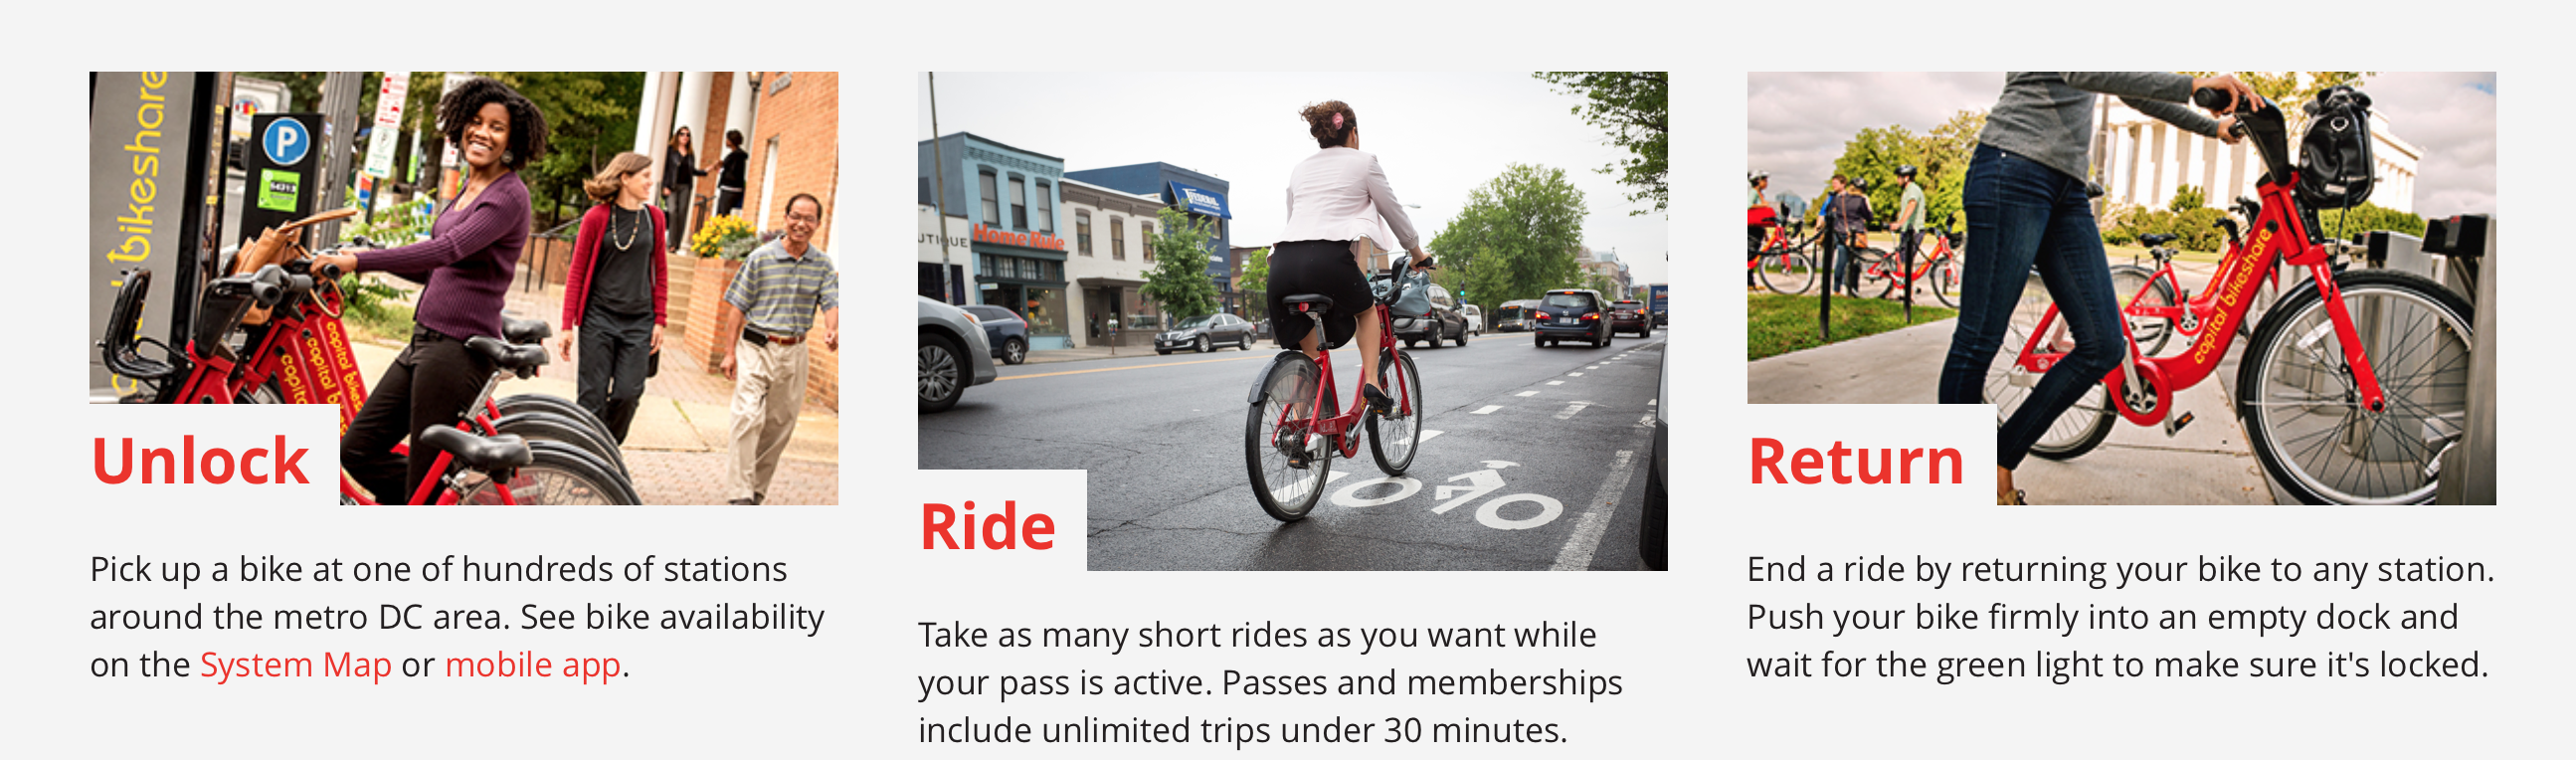
\includegraphics{fig/BSS.png}
\caption{bike\_sharing}
\end{figure}

Main Theme: Multiple Linear Regression, Subset Selection, Polynomial
Regression

\subsubsection{Overview}\label{overview}

You are hired by the administrators of the
\href{https://www.capitalbikeshare.com}{Capital Bikeshare program}
program in Washington D.C., to \textbf{help them predict the hourly
demand for rental bikes} and \textbf{give them suggestions on how to
increase their revenue}. Your task is to prepare a short report
summarizing your findings and make recommendations.

The predicted hourly demand could be used for planning the number of
bikes that need to be available in the system at any given hour of the
day. It costs the program money if bike stations are full and bikes
cannot be returned, or empty and there are no bikes available. You will
use multiple linear regression and polynomial regression and will
explore techniques for subset selection to predict bike usage. The goal
is to build a regression model that can predict the total number of bike
rentals in a given hour of the day, based on all available information
given to you.

An example of a suggestion to increase revenue might be to offer
discounts during certain times of the day either during holidays or
non-holidays. Your suggestions will depend on your observations of the
seasonality of ridership.

The data for this problem were collected from the Capital Bikeshare
program over the course of two years (2011 and 2012).

    \subsubsection{Use only the libraries
below:}\label{use-only-the-libraries-below}

    \begin{Verbatim}[commandchars=\\\{\}]
{\color{incolor}In [{\color{incolor}2}]:} \PY{k+kn}{import} \PY{n+nn}{numpy} \PY{k}{as} \PY{n+nn}{np}
        \PY{k+kn}{import} \PY{n+nn}{pandas} \PY{k}{as} \PY{n+nn}{pd}
        \PY{k+kn}{import} \PY{n+nn}{matplotlib}
        \PY{k+kn}{import} \PY{n+nn}{matplotlib}\PY{n+nn}{.}\PY{n+nn}{pyplot} \PY{k}{as} \PY{n+nn}{plt}
        
        \PY{k+kn}{import} \PY{n+nn}{statsmodels}\PY{n+nn}{.}\PY{n+nn}{api} \PY{k}{as} \PY{n+nn}{sm}
        \PY{k+kn}{from} \PY{n+nn}{statsmodels}\PY{n+nn}{.}\PY{n+nn}{api} \PY{k}{import} \PY{n}{OLS}
        
        \PY{k+kn}{from} \PY{n+nn}{sklearn} \PY{k}{import} \PY{n}{preprocessing}
        \PY{k+kn}{from} \PY{n+nn}{sklearn}\PY{n+nn}{.}\PY{n+nn}{preprocessing} \PY{k}{import} \PY{n}{PolynomialFeatures}
        \PY{k+kn}{from} \PY{n+nn}{sklearn}\PY{n+nn}{.}\PY{n+nn}{metrics} \PY{k}{import} \PY{n}{r2\PYZus{}score}
        \PY{k+kn}{from} \PY{n+nn}{sklearn}\PY{n+nn}{.}\PY{n+nn}{model\PYZus{}selection} \PY{k}{import} \PY{n}{train\PYZus{}test\PYZus{}split}
        
        \PY{k+kn}{from} \PY{n+nn}{pandas}\PY{n+nn}{.}\PY{n+nn}{plotting} \PY{k}{import} \PY{n}{scatter\PYZus{}matrix}
        
        \PY{k+kn}{import} \PY{n+nn}{seaborn} \PY{k}{as} \PY{n+nn}{sns}
        
        
        \PY{o}{\PYZpc{}}\PY{k}{matplotlib} inline
\end{Verbatim}


    \subsection{Data Exploration \& Preprocessing, Multiple Linear
Regression, Subset
Selection}\label{data-exploration-preprocessing-multiple-linear-regression-subset-selection}

    \subsubsection{Overview}\label{overview}

The initial data set is provided in the file
\texttt{data/BSS\_hour\_raw.csv}. You will first add features that will
help with the analysis and then separate the data into training and test
sets. Each row in this file represents the number of rides by registered
users and casual users in a given hour of a specific date. There are 12
attributes in total describing besides the number of users the weather
if it is a holiday or not etc:

\begin{itemize}
\tightlist
\item
  \texttt{dteday} (date in the format YYYY-MM-DD, e.g. 2011-01-01)
\item
  \texttt{season} (1 = winter, 2 = spring, 3 = summer, 4 = fall)
\item
  \texttt{hour} (0 for 12 midnight, 1 for 1:00am, 23 for 11:00pm)
\item
  \texttt{weekday} (0 through 6, with 0 denoting Sunday)
\item
  \texttt{holiday} (1 = the day is a holiday, 0 = otherwise)
\item
  \texttt{weather}

  \begin{itemize}
  \tightlist
  \item
    1: Clear, Few clouds, Partly cloudy, Partly cloudy
  \item
    2: Mist + Cloudy, Mist + Broken clouds, Mist + Few clouds, Mist
  \item
    3: Light Snow, Light Rain + Thunderstorm
  \item
    4: Heavy Rain + Thunderstorm + Mist, Snow + Fog
  \end{itemize}
\item
  \texttt{temp} (temperature in Celsius)
\item
  \texttt{atemp} (apparent temperature, or relative outdoor temperature,
  in Celsius)
\item
  \texttt{hum} (relative humidity)
\item
  \texttt{windspeed} (wind speed)
\item
  \texttt{casual} (number of rides that day made by casual riders, not
  registered in the system)
\item
  \texttt{registered} (number of rides that day made by registered
  riders)
\end{itemize}

    \subsubsection{General Hints}\label{general-hints}

\begin{itemize}
\tightlist
\item
  Use pandas .describe() to see statistics for the dataset.
\item
  When performing manipulations on column data it is useful and often
  more efficient to write a function and apply this function to the
  column as a whole without the need for iterating through the elements.
\item
  A scatterplot matrix or correlation matrix are both good ways to see
  dependencies between multiple variables.
\item
  For Question 2, a very useful pandas method is .groupby(). Make sure
  you aggregate the rest of the columns in a meaningful way. Print the
  dataframe to make sure all variables/columns are there!
\end{itemize}

\subsubsection{Resources}\label{resources}

http://pandas.pydata.org/pandas-docs/stable/generated/pandas.to\_datetime.html

     Question 1: Data Read-In and Cleaning

In this section, we read in the data and begin one of the most important
analytic steps: verifying that the data is what it claims to be.

\textbf{1.1} Load the dataset from the csv file
\texttt{data/BSS\_hour\_raw.csv} into a pandas dataframe that you name
\texttt{bikes\_df}. Do any of the variables' ranges or averages seem
suspect? Do the data types make sense?

\textbf{1.2} Notice that the variable in column \texttt{dteday} is a
pandas \texttt{object}, which is \textbf{not} useful when you want to
extract the elements of the date such as the year, month, and day.
Convert \texttt{dteday} into a \texttt{datetime} object to prepare it
for later analysis.

\textbf{1.3} Create three new columns in the dataframe: - \texttt{year}
with 0 for 2011, 1 for 2012, etc. - \texttt{month} with 1 through 12,
with 1 denoting January. - \texttt{counts} with the total number of bike
rentals for that \textbf{hour} (this is the response variable for
later).

    \subsubsection{Answers}\label{answers}

    \paragraph{\texorpdfstring{\textbf{1.1} Load the dataset from the csv
file \texttt{data/BSS\_hour\_raw.csv} into a pandas dataframe that you
name \texttt{bikes\_df}. Do any of the variables' ranges or averages
seem suspect? Do the data types make
sense?}{1.1 Load the dataset from the csv file data/BSS\_hour\_raw.csv into a pandas dataframe that you name bikes\_df. Do any of the variables' ranges or averages seem suspect? Do the data types make sense?}}\label{load-the-dataset-from-the-csv-file-databss_hour_raw.csv-into-a-pandas-dataframe-that-you-name-bikes_df.-do-any-of-the-variables-ranges-or-averages-seem-suspect-do-the-data-types-make-sense}

    \begin{Verbatim}[commandchars=\\\{\}]
{\color{incolor}In [{\color{incolor}3}]:} \PY{c+c1}{\PYZsh{} your code here}
        \PY{n}{bikes\PYZus{}df} \PY{o}{=} \PY{n}{pd}\PY{o}{.}\PY{n}{read\PYZus{}csv}\PY{p}{(}\PY{l+s+s1}{\PYZsq{}}\PY{l+s+s1}{data/BSS\PYZus{}hour\PYZus{}raw.csv}\PY{l+s+s1}{\PYZsq{}}\PY{p}{,} \PY{n}{delimiter}\PY{o}{=}\PY{l+s+s1}{\PYZsq{}}\PY{l+s+s1}{,}\PY{l+s+s1}{\PYZsq{}}\PY{p}{)}
        \PY{n}{bikes\PYZus{}df}\PY{o}{.}\PY{n}{shape}
\end{Verbatim}


\begin{Verbatim}[commandchars=\\\{\}]
{\color{outcolor}Out[{\color{outcolor}3}]:} (17379, 13)
\end{Verbatim}
            
    \begin{Verbatim}[commandchars=\\\{\}]
{\color{incolor}In [{\color{incolor}4}]:} \PY{c+c1}{\PYZsh{} your code here}
        \PY{n}{bikes\PYZus{}df}\PY{o}{.}\PY{n}{dtypes}
\end{Verbatim}


\begin{Verbatim}[commandchars=\\\{\}]
{\color{outcolor}Out[{\color{outcolor}4}]:} dteday         object
        season          int64
        hour            int64
        holiday         int64
        weekday         int64
        workingday      int64
        weather         int64
        temp          float64
        atemp         float64
        hum           float64
        windspeed     float64
        casual          int64
        registered      int64
        dtype: object
\end{Verbatim}
            
    \begin{Verbatim}[commandchars=\\\{\}]
{\color{incolor}In [{\color{incolor}5}]:} \PY{c+c1}{\PYZsh{} your code here}
        \PY{n}{bikes\PYZus{}df}\PY{o}{.}\PY{n}{describe}\PY{p}{(}\PY{p}{)}
\end{Verbatim}


\begin{Verbatim}[commandchars=\\\{\}]
{\color{outcolor}Out[{\color{outcolor}5}]:}              season          hour       holiday       weekday    workingday  \textbackslash{}
        count  17379.000000  17379.000000  17379.000000  17379.000000  17379.000000   
        mean       2.501640     11.546752      0.028770      3.003683      0.682721   
        std        1.106918      6.914405      0.167165      2.005771      0.465431   
        min        1.000000      0.000000      0.000000      0.000000      0.000000   
        25\%        2.000000      6.000000      0.000000      1.000000      0.000000   
        50\%        3.000000     12.000000      0.000000      3.000000      1.000000   
        75\%        3.000000     18.000000      0.000000      5.000000      1.000000   
        max        4.000000     23.000000      1.000000      6.000000      1.000000   
        
                    weather          temp         atemp           hum     windspeed  \textbackslash{}
        count  17379.000000  17379.000000  17379.000000  17379.000000  17379.000000   
        mean       1.425283      0.496987      0.475775      0.627229      0.190098   
        std        0.639357      0.192556      0.171850      0.192930      0.122340   
        min        1.000000      0.020000      0.000000      0.000000      0.000000   
        25\%        1.000000      0.340000      0.333300      0.480000      0.104500   
        50\%        1.000000      0.500000      0.484800      0.630000      0.194000   
        75\%        2.000000      0.660000      0.621200      0.780000      0.253700   
        max        4.000000      1.000000      1.000000      1.000000      0.850700   
        
                     casual    registered  
        count  17379.000000  17379.000000  
        mean      35.676218    153.786869  
        std       49.305030    151.357286  
        min        0.000000      0.000000  
        25\%        4.000000     34.000000  
        50\%       17.000000    115.000000  
        75\%       48.000000    220.000000  
        max      367.000000    886.000000  
\end{Verbatim}
            
    \textbf{Answer:}

\emph{We observe that maximum for 'casual' and 'registered' are way
higher considering their mean and standard deviation. That means we have
some outliers there. Also, 'temp', 'hum', 'atemp' and 'windspeed are all
between \(0\) and \(1\), which means that they are normalized.}

    \paragraph{\texorpdfstring{\textbf{1.2} Notice that the variable in
column \texttt{dteday} is a pandas \texttt{object}, which is
\textbf{not} useful when you want to extract the elements of the date
such as the year, month, and day. Convert \texttt{dteday} into a
\texttt{datetime} object to prepare it for later
analysis.}{1.2 Notice that the variable in column dteday is a pandas object, which is not useful when you want to extract the elements of the date such as the year, month, and day. Convert dteday into a datetime object to prepare it for later analysis.}}\label{notice-that-the-variable-in-column-dteday-is-a-pandas-object-which-is-not-useful-when-you-want-to-extract-the-elements-of-the-date-such-as-the-year-month-and-day.-convert-dteday-into-a-datetime-object-to-prepare-it-for-later-analysis.}

    \begin{Verbatim}[commandchars=\\\{\}]
{\color{incolor}In [{\color{incolor}6}]:} \PY{c+c1}{\PYZsh{} your code here}
        \PY{n}{bikes\PYZus{}df}\PY{p}{[}\PY{l+s+s1}{\PYZsq{}}\PY{l+s+s1}{dteday}\PY{l+s+s1}{\PYZsq{}}\PY{p}{]} \PY{o}{=} \PY{n}{pd}\PY{o}{.}\PY{n}{to\PYZus{}datetime}\PY{p}{(}\PY{n}{bikes\PYZus{}df}\PY{p}{[}\PY{l+s+s1}{\PYZsq{}}\PY{l+s+s1}{dteday}\PY{l+s+s1}{\PYZsq{}}\PY{p}{]}\PY{p}{)}
\end{Verbatim}


    \paragraph{\texorpdfstring{\textbf{1.3} Create three new columns in the
dataframe:}{1.3 Create three new columns in the dataframe:}}\label{create-three-new-columns-in-the-dataframe}

\begin{itemize}
\tightlist
\item
  \texttt{year} with 0 for 2011, 1 for 2012, etc.
\item
  \texttt{month} with 1 through 12, with 1 denoting January.
\item
  \texttt{counts} with the total number of bike rentals for that hour
  (this is the response variable for later).
\end{itemize}

    \begin{Verbatim}[commandchars=\\\{\}]
{\color{incolor}In [{\color{incolor}7}]:} \PY{c+c1}{\PYZsh{} your code here}
        \PY{n}{bikes\PYZus{}df}\PY{p}{[}\PY{l+s+s1}{\PYZsq{}}\PY{l+s+s1}{year}\PY{l+s+s1}{\PYZsq{}}\PY{p}{]} \PY{o}{=} \PY{n}{bikes\PYZus{}df}\PY{p}{[}\PY{l+s+s1}{\PYZsq{}}\PY{l+s+s1}{dteday}\PY{l+s+s1}{\PYZsq{}}\PY{p}{]}\PY{o}{.}\PY{n}{dt}\PY{o}{.}\PY{n}{year} \PY{o}{\PYZhy{}} \PY{l+m+mi}{2011}
        \PY{n}{bikes\PYZus{}df}\PY{p}{[}\PY{l+s+s1}{\PYZsq{}}\PY{l+s+s1}{month}\PY{l+s+s1}{\PYZsq{}}\PY{p}{]} \PY{o}{=} \PY{n}{bikes\PYZus{}df}\PY{p}{[}\PY{l+s+s1}{\PYZsq{}}\PY{l+s+s1}{dteday}\PY{l+s+s1}{\PYZsq{}}\PY{p}{]}\PY{o}{.}\PY{n}{dt}\PY{o}{.}\PY{n}{month}
        \PY{n}{bikes\PYZus{}df}\PY{p}{[}\PY{l+s+s1}{\PYZsq{}}\PY{l+s+s1}{counts}\PY{l+s+s1}{\PYZsq{}}\PY{p}{]} \PY{o}{=} \PY{n}{bikes\PYZus{}df}\PY{p}{[}\PY{l+s+s1}{\PYZsq{}}\PY{l+s+s1}{casual}\PY{l+s+s1}{\PYZsq{}}\PY{p}{]} \PY{o}{+} \PY{n}{bikes\PYZus{}df}\PY{p}{[}\PY{l+s+s1}{\PYZsq{}}\PY{l+s+s1}{registered}\PY{l+s+s1}{\PYZsq{}}\PY{p}{]}
\end{Verbatim}


    \begin{Verbatim}[commandchars=\\\{\}]
{\color{incolor}In [{\color{incolor}8}]:} \PY{c+c1}{\PYZsh{} your code here}
        \PY{n}{bikes\PYZus{}df}\PY{o}{.}\PY{n}{head}\PY{p}{(}\PY{p}{)}
\end{Verbatim}


\begin{Verbatim}[commandchars=\\\{\}]
{\color{outcolor}Out[{\color{outcolor}8}]:}       dteday  season  hour  holiday  weekday  workingday  weather  temp  \textbackslash{}
        0 2011-01-01       1     0        0        6           0        1  0.24   
        1 2011-01-01       1     1        0        6           0        1  0.22   
        2 2011-01-01       1     2        0        6           0        1  0.22   
        3 2011-01-01       1     3        0        6           0        1  0.24   
        4 2011-01-01       1     4        0        6           0        1  0.24   
        
            atemp   hum  windspeed  casual  registered  year  month  counts  
        0  0.2879  0.81        0.0       3          13     0      1      16  
        1  0.2727  0.80        0.0       8          32     0      1      40  
        2  0.2727  0.80        0.0       5          27     0      1      32  
        3  0.2879  0.75        0.0       3          10     0      1      13  
        4  0.2879  0.75        0.0       0           1     0      1       1  
\end{Verbatim}
            
     Question 2: Exploratory Data Analysis.

In this question, we continue validating the data, and begin hunting for
patterns in ridership that shed light on who uses the service and why.

\textbf{2.1} Use pandas' \texttt{scatter\_matrix} command to visualize
the inter-dependencies among all predictors in the dataset. Note and
comment on any strongly related variables. {[}This will take several
minutes to run. You may wish to comment it out until your final
submission, or only plot a randomly-selected 10\% of the rows{]}

\textbf{2.2} Make a plot showing the \emph{average} number of casual and
registered riders during each hour of the day. \texttt{.groupby} and
\texttt{.aggregate} should make this task easy. Comment on the trends
you observe.

\textbf{2.3} Use the variable \texttt{weather} to show how each weather
category affects the relationships in question 2.2. What do you observe?

\textbf{2.4} Make a new dataframe with the following subset of
attributes from the previous dataset and with each entry being just
\textbf{one} day:

\begin{itemize}
\tightlist
\item
  \texttt{dteday}, the timestamp for that day (fine to set to noon or
  any other time)
\item
  \texttt{weekday}, the day of the week
\item
  \texttt{weather}, the most severe weather that day
\item
  \texttt{season}, the season that day falls in
\item
  \texttt{temp}, the average temperature (normalized)
\item
  \texttt{atemp}, the average atemp that day (normalized)
\item
  \texttt{windspeed}, the average windspeed that day (normalized)
\item
  \texttt{hum}, the average humidity that day (normalized)
\item
  \texttt{casual}, the \textbf{total} number of rentals by casual users
\item
  \texttt{registered}, the \textbf{total} number of rentals by
  registered users
\item
  \texttt{counts}, the \textbf{total} number of rentals of that day
\end{itemize}

Name this dataframe \texttt{bikes\_by\_day}.

Make a plot showing the \emph{distribution} of the number of casual and
registered riders on each day of the week.

\textbf{2.5} Use \texttt{bikes\_by\_day} to visualize how the
distribution of \textbf{total number of rides} per day (casual and
registered riders combined) varies with the \textbf{season}. Do you see
any \textbf{outliers}? Here we use the pyplot's boxplot function
definition of an outlier as any value 1.5 times the IQR above the 75th
percentile or 1.5 times the IQR below the 25th percentiles. If you see
any outliers, identify those dates and investigate if they are a chance
occurence, an error in the data collection, or a significant event (an
online search of those date(s) might help).

    \subsubsection{Answers}\label{answers}

    \paragraph{\texorpdfstring{\textbf{2.1} Use pandas'
\texttt{scatter\_matrix} command to visualize the inter-dependencies
among all predictors in the dataset. Note and comment on any strongly
related variables. {[}This will take several minutes to run. You may
wish to comment it out until your final submission, or only plot a
randomly-selected 10\% of the
rows{]}}{2.1 Use pandas' scatter\_matrix command to visualize the inter-dependencies among all predictors in the dataset. Note and comment on any strongly related variables. {[}This will take several minutes to run. You may wish to comment it out until your final submission, or only plot a randomly-selected 10\% of the rows{]}}}\label{use-pandas-scatter_matrix-command-to-visualize-the-inter-dependencies-among-all-predictors-in-the-dataset.-note-and-comment-on-any-strongly-related-variables.-this-will-take-several-minutes-to-run.-you-may-wish-to-comment-it-out-until-your-final-submission-or-only-plot-a-randomly-selected-10-of-the-rows}

    \begin{Verbatim}[commandchars=\\\{\}]
{\color{incolor}In [{\color{incolor}9}]:} \PY{c+c1}{\PYZsh{} your code here}
        \PY{n}{pd}\PY{o}{.}\PY{n}{plotting}\PY{o}{.}\PY{n}{scatter\PYZus{}matrix}\PY{p}{(}\PY{n}{bikes\PYZus{}df}\PY{p}{,} \PY{n}{figsize} \PY{o}{=} \PY{p}{(}\PY{l+m+mi}{15}\PY{p}{,}\PY{l+m+mi}{15}\PY{p}{)}\PY{p}{,} \PY{n}{grid} \PY{o}{=} \PY{k+kc}{True}\PY{p}{)}
\end{Verbatim}


\begin{Verbatim}[commandchars=\\\{\}]
{\color{outcolor}Out[{\color{outcolor}9}]:} array([[<matplotlib.axes.\_subplots.AxesSubplot object at 0x00000002E324CF28>,
                <matplotlib.axes.\_subplots.AxesSubplot object at 0x00000002E348A630>,
                <matplotlib.axes.\_subplots.AxesSubplot object at 0x00000002E34BC940>,
                <matplotlib.axes.\_subplots.AxesSubplot object at 0x00000002E3520C50>,
                <matplotlib.axes.\_subplots.AxesSubplot object at 0x00000002E34D1E80>,
                <matplotlib.axes.\_subplots.AxesSubplot object at 0x00000002E34D1EB8>,
                <matplotlib.axes.\_subplots.AxesSubplot object at 0x00000002E346D630>,
                <matplotlib.axes.\_subplots.AxesSubplot object at 0x00000002E3593CC0>,
                <matplotlib.axes.\_subplots.AxesSubplot object at 0x00000002E3603390>,
                <matplotlib.axes.\_subplots.AxesSubplot object at 0x00000002E3629A20>,
                <matplotlib.axes.\_subplots.AxesSubplot object at 0x00000002E36EC0F0>,
                <matplotlib.axes.\_subplots.AxesSubplot object at 0x00000002E3713780>,
                <matplotlib.axes.\_subplots.AxesSubplot object at 0x00000002E373AE10>,
                <matplotlib.axes.\_subplots.AxesSubplot object at 0x00000002E376A4E0>,
                <matplotlib.axes.\_subplots.AxesSubplot object at 0x00000002E3791B70>],
               [<matplotlib.axes.\_subplots.AxesSubplot object at 0x00000002E37C3240>,
                <matplotlib.axes.\_subplots.AxesSubplot object at 0x00000002E47B88D0>,
                <matplotlib.axes.\_subplots.AxesSubplot object at 0x00000002E47E3F28>,
                <matplotlib.axes.\_subplots.AxesSubplot object at 0x00000002E48135F8>,
                <matplotlib.axes.\_subplots.AxesSubplot object at 0x00000002E483BC88>,
                <matplotlib.axes.\_subplots.AxesSubplot object at 0x00000002E489C358>,
                <matplotlib.axes.\_subplots.AxesSubplot object at 0x00000002E48C49E8>,
                <matplotlib.axes.\_subplots.AxesSubplot object at 0x00000002E48F50B8>,
                <matplotlib.axes.\_subplots.AxesSubplot object at 0x00000002E491D748>,
                <matplotlib.axes.\_subplots.AxesSubplot object at 0x00000002E4944DD8>,
                <matplotlib.axes.\_subplots.AxesSubplot object at 0x00000002E49744A8>,
                <matplotlib.axes.\_subplots.AxesSubplot object at 0x00000002E499CB38>,
                <matplotlib.axes.\_subplots.AxesSubplot object at 0x00000002E49CE208>,
                <matplotlib.axes.\_subplots.AxesSubplot object at 0x00000002E49F6898>,
                <matplotlib.axes.\_subplots.AxesSubplot object at 0x00000002E4D9EF28>],
               [<matplotlib.axes.\_subplots.AxesSubplot object at 0x00000002E4DCE5F8>,
                <matplotlib.axes.\_subplots.AxesSubplot object at 0x00000002E4DF4C88>,
                <matplotlib.axes.\_subplots.AxesSubplot object at 0x00000002E4E28358>,
                <matplotlib.axes.\_subplots.AxesSubplot object at 0x00000002E4E4F9E8>,
                <matplotlib.axes.\_subplots.AxesSubplot object at 0x00000002E4E800B8>,
                <matplotlib.axes.\_subplots.AxesSubplot object at 0x00000002E4EAA748>,
                <matplotlib.axes.\_subplots.AxesSubplot object at 0x00000002E4ED1DD8>,
                <matplotlib.axes.\_subplots.AxesSubplot object at 0x00000002E4F004A8>,
                <matplotlib.axes.\_subplots.AxesSubplot object at 0x00000002E4F29B38>,
                <matplotlib.axes.\_subplots.AxesSubplot object at 0x00000002E4F59208>,
                <matplotlib.axes.\_subplots.AxesSubplot object at 0x00000002E4F81898>,
                <matplotlib.axes.\_subplots.AxesSubplot object at 0x00000002E4FAAF28>,
                <matplotlib.axes.\_subplots.AxesSubplot object at 0x00000002E4FDB5F8>,
                <matplotlib.axes.\_subplots.AxesSubplot object at 0x00000002E5003C88>,
                <matplotlib.axes.\_subplots.AxesSubplot object at 0x00000002E5033358>],
               [<matplotlib.axes.\_subplots.AxesSubplot object at 0x00000002E505A9E8>,
                <matplotlib.axes.\_subplots.AxesSubplot object at 0x00000002E508D0B8>,
                <matplotlib.axes.\_subplots.AxesSubplot object at 0x00000002E50B3748>,
                <matplotlib.axes.\_subplots.AxesSubplot object at 0x00000002E50DCDD8>,
                <matplotlib.axes.\_subplots.AxesSubplot object at 0x00000002E510C4A8>,
                <matplotlib.axes.\_subplots.AxesSubplot object at 0x00000002E5134B38>,
                <matplotlib.axes.\_subplots.AxesSubplot object at 0x00000002E5165208>,
                <matplotlib.axes.\_subplots.AxesSubplot object at 0x00000002E518C898>,
                <matplotlib.axes.\_subplots.AxesSubplot object at 0x00000002E51B5F28>,
                <matplotlib.axes.\_subplots.AxesSubplot object at 0x00000002E51E55F8>,
                <matplotlib.axes.\_subplots.AxesSubplot object at 0x00000002E520DC88>,
                <matplotlib.axes.\_subplots.AxesSubplot object at 0x00000002E523E358>,
                <matplotlib.axes.\_subplots.AxesSubplot object at 0x00000002E52679E8>,
                <matplotlib.axes.\_subplots.AxesSubplot object at 0x00000002E52980B8>,
                <matplotlib.axes.\_subplots.AxesSubplot object at 0x00000002E52C0748>],
               [<matplotlib.axes.\_subplots.AxesSubplot object at 0x00000002E52E9DD8>,
                <matplotlib.axes.\_subplots.AxesSubplot object at 0x00000002E53184A8>,
                <matplotlib.axes.\_subplots.AxesSubplot object at 0x00000002E533EB38>,
                <matplotlib.axes.\_subplots.AxesSubplot object at 0x00000002E5371208>,
                <matplotlib.axes.\_subplots.AxesSubplot object at 0x00000002E5398898>,
                <matplotlib.axes.\_subplots.AxesSubplot object at 0x00000002E53BFF28>,
                <matplotlib.axes.\_subplots.AxesSubplot object at 0x00000002E53F15F8>,
                <matplotlib.axes.\_subplots.AxesSubplot object at 0x00000002E5417C88>,
                <matplotlib.axes.\_subplots.AxesSubplot object at 0x00000002E544A358>,
                <matplotlib.axes.\_subplots.AxesSubplot object at 0x00000002E54729E8>,
                <matplotlib.axes.\_subplots.AxesSubplot object at 0x00000002E54A30B8>,
                <matplotlib.axes.\_subplots.AxesSubplot object at 0x00000002E54C9748>,
                <matplotlib.axes.\_subplots.AxesSubplot object at 0x00000002E54F1DD8>,
                <matplotlib.axes.\_subplots.AxesSubplot object at 0x00000002E55224A8>,
                <matplotlib.axes.\_subplots.AxesSubplot object at 0x00000002E5549B38>],
               [<matplotlib.axes.\_subplots.AxesSubplot object at 0x00000002E557D208>,
                <matplotlib.axes.\_subplots.AxesSubplot object at 0x00000002E55A4898>,
                <matplotlib.axes.\_subplots.AxesSubplot object at 0x00000002E55CCF28>,
                <matplotlib.axes.\_subplots.AxesSubplot object at 0x00000002E55FA5F8>,
                <matplotlib.axes.\_subplots.AxesSubplot object at 0x00000002E5623C88>,
                <matplotlib.axes.\_subplots.AxesSubplot object at 0x00000002E5655358>,
                <matplotlib.axes.\_subplots.AxesSubplot object at 0x00000002E567B9E8>,
                <matplotlib.axes.\_subplots.AxesSubplot object at 0x00000002E56AF0B8>,
                <matplotlib.axes.\_subplots.AxesSubplot object at 0x00000002E56D6748>,
                <matplotlib.axes.\_subplots.AxesSubplot object at 0x00000002E56FDDD8>,
                <matplotlib.axes.\_subplots.AxesSubplot object at 0x00000002E572D4A8>,
                <matplotlib.axes.\_subplots.AxesSubplot object at 0x00000002E5757B38>,
                <matplotlib.axes.\_subplots.AxesSubplot object at 0x00000002E5787208>,
                <matplotlib.axes.\_subplots.AxesSubplot object at 0x00000002E57AE898>,
                <matplotlib.axes.\_subplots.AxesSubplot object at 0x00000002E67A7F28>],
               [<matplotlib.axes.\_subplots.AxesSubplot object at 0x00000002E67D65F8>,
                <matplotlib.axes.\_subplots.AxesSubplot object at 0x00000002E67FEC88>,
                <matplotlib.axes.\_subplots.AxesSubplot object at 0x00000002E682F358>,
                <matplotlib.axes.\_subplots.AxesSubplot object at 0x00000002E68589E8>,
                <matplotlib.axes.\_subplots.AxesSubplot object at 0x00000002E68890B8>,
                <matplotlib.axes.\_subplots.AxesSubplot object at 0x00000002E68B0748>,
                <matplotlib.axes.\_subplots.AxesSubplot object at 0x00000002E68D7DD8>,
                <matplotlib.axes.\_subplots.AxesSubplot object at 0x00000002E69094A8>,
                <matplotlib.axes.\_subplots.AxesSubplot object at 0x00000002E692FB38>,
                <matplotlib.axes.\_subplots.AxesSubplot object at 0x00000002E6963208>,
                <matplotlib.axes.\_subplots.AxesSubplot object at 0x00000002E698A898>,
                <matplotlib.axes.\_subplots.AxesSubplot object at 0x00000002E69B2F28>,
                <matplotlib.axes.\_subplots.AxesSubplot object at 0x00000002E69E25F8>,
                <matplotlib.axes.\_subplots.AxesSubplot object at 0x00000002E6A09C88>,
                <matplotlib.axes.\_subplots.AxesSubplot object at 0x00000002E6A3C358>],
               [<matplotlib.axes.\_subplots.AxesSubplot object at 0x00000002E6A629E8>,
                <matplotlib.axes.\_subplots.AxesSubplot object at 0x00000002E6A940B8>,
                <matplotlib.axes.\_subplots.AxesSubplot object at 0x00000002E6ABC748>,
                <matplotlib.axes.\_subplots.AxesSubplot object at 0x00000002E6AE5DD8>,
                <matplotlib.axes.\_subplots.AxesSubplot object at 0x00000002E6B144A8>,
                <matplotlib.axes.\_subplots.AxesSubplot object at 0x00000002E6B3DB38>,
                <matplotlib.axes.\_subplots.AxesSubplot object at 0x00000002E6B6E208>,
                <matplotlib.axes.\_subplots.AxesSubplot object at 0x00000002E6B95898>,
                <matplotlib.axes.\_subplots.AxesSubplot object at 0x00000002E6BBDF28>,
                <matplotlib.axes.\_subplots.AxesSubplot object at 0x00000002E6BEE5F8>,
                <matplotlib.axes.\_subplots.AxesSubplot object at 0x00000002E6C14C88>,
                <matplotlib.axes.\_subplots.AxesSubplot object at 0x00000002E6C46358>,
                <matplotlib.axes.\_subplots.AxesSubplot object at 0x00000002E6C6E9E8>,
                <matplotlib.axes.\_subplots.AxesSubplot object at 0x00000002E6C9F0B8>,
                <matplotlib.axes.\_subplots.AxesSubplot object at 0x00000002E6CC7748>],
               [<matplotlib.axes.\_subplots.AxesSubplot object at 0x00000002E6CEEDD8>,
                <matplotlib.axes.\_subplots.AxesSubplot object at 0x00000002E6D1F4A8>,
                <matplotlib.axes.\_subplots.AxesSubplot object at 0x00000002E6D47B38>,
                <matplotlib.axes.\_subplots.AxesSubplot object at 0x00000002E6D7B208>,
                <matplotlib.axes.\_subplots.AxesSubplot object at 0x00000002E6DA0898>,
                <matplotlib.axes.\_subplots.AxesSubplot object at 0x00000002E6DCAF28>,
                <matplotlib.axes.\_subplots.AxesSubplot object at 0x00000002E6DFA5F8>,
                <matplotlib.axes.\_subplots.AxesSubplot object at 0x00000002E6E23C88>,
                <matplotlib.axes.\_subplots.AxesSubplot object at 0x00000002E6E52358>,
                <matplotlib.axes.\_subplots.AxesSubplot object at 0x00000002E6E7B9E8>,
                <matplotlib.axes.\_subplots.AxesSubplot object at 0x00000002E6EAA0B8>,
                <matplotlib.axes.\_subplots.AxesSubplot object at 0x00000002E6ED2748>,
                <matplotlib.axes.\_subplots.AxesSubplot object at 0x00000002E6EFCDD8>,
                <matplotlib.axes.\_subplots.AxesSubplot object at 0x00000002E6F2D4A8>,
                <matplotlib.axes.\_subplots.AxesSubplot object at 0x00000002E6F53B38>],
               [<matplotlib.axes.\_subplots.AxesSubplot object at 0x00000002E6F86208>,
                <matplotlib.axes.\_subplots.AxesSubplot object at 0x00000002E6FAC898>,
                <matplotlib.axes.\_subplots.AxesSubplot object at 0x00000002E6FD3F28>,
                <matplotlib.axes.\_subplots.AxesSubplot object at 0x00000002E70055F8>,
                <matplotlib.axes.\_subplots.AxesSubplot object at 0x00000002E702EC88>,
                <matplotlib.axes.\_subplots.AxesSubplot object at 0x00000002E705F358>,
                <matplotlib.axes.\_subplots.AxesSubplot object at 0x00000002E70859E8>,
                <matplotlib.axes.\_subplots.AxesSubplot object at 0x00000002E70B70B8>,
                <matplotlib.axes.\_subplots.AxesSubplot object at 0x00000002E70DE748>,
                <matplotlib.axes.\_subplots.AxesSubplot object at 0x00000002E7104DD8>,
                <matplotlib.axes.\_subplots.AxesSubplot object at 0x00000002E71374A8>,
                <matplotlib.axes.\_subplots.AxesSubplot object at 0x00000002E715EB38>,
                <matplotlib.axes.\_subplots.AxesSubplot object at 0x00000002E7190208>,
                <matplotlib.axes.\_subplots.AxesSubplot object at 0x00000002E71B8898>,
                <matplotlib.axes.\_subplots.AxesSubplot object at 0x00000002E71E0F28>],
               [<matplotlib.axes.\_subplots.AxesSubplot object at 0x00000002E72105F8>,
                <matplotlib.axes.\_subplots.AxesSubplot object at 0x00000002E7238C88>,
                <matplotlib.axes.\_subplots.AxesSubplot object at 0x00000002E726B358>,
                <matplotlib.axes.\_subplots.AxesSubplot object at 0x00000002E728F9E8>,
                <matplotlib.axes.\_subplots.AxesSubplot object at 0x00000002E72C10B8>,
                <matplotlib.axes.\_subplots.AxesSubplot object at 0x00000002E72EB748>,
                <matplotlib.axes.\_subplots.AxesSubplot object at 0x00000002E7312DD8>,
                <matplotlib.axes.\_subplots.AxesSubplot object at 0x00000002E73424A8>,
                <matplotlib.axes.\_subplots.AxesSubplot object at 0x00000002E736BB38>,
                <matplotlib.axes.\_subplots.AxesSubplot object at 0x00000002E739D208>,
                <matplotlib.axes.\_subplots.AxesSubplot object at 0x00000002E73C1898>,
                <matplotlib.axes.\_subplots.AxesSubplot object at 0x00000002E73EBF28>,
                <matplotlib.axes.\_subplots.AxesSubplot object at 0x00000002E741C5F8>,
                <matplotlib.axes.\_subplots.AxesSubplot object at 0x00000002E7444C88>,
                <matplotlib.axes.\_subplots.AxesSubplot object at 0x00000002E7474358>],
               [<matplotlib.axes.\_subplots.AxesSubplot object at 0x00000002E749E9E8>,
                <matplotlib.axes.\_subplots.AxesSubplot object at 0x00000002E74CD0B8>,
                <matplotlib.axes.\_subplots.AxesSubplot object at 0x00000002E74F3748>,
                <matplotlib.axes.\_subplots.AxesSubplot object at 0x00000002E751EDD8>,
                <matplotlib.axes.\_subplots.AxesSubplot object at 0x00000002E754D4A8>,
                <matplotlib.axes.\_subplots.AxesSubplot object at 0x00000002E7573B38>,
                <matplotlib.axes.\_subplots.AxesSubplot object at 0x00000002E75A7208>,
                <matplotlib.axes.\_subplots.AxesSubplot object at 0x00000002E75CF898>,
                <matplotlib.axes.\_subplots.AxesSubplot object at 0x00000002E75F6F28>,
                <matplotlib.axes.\_subplots.AxesSubplot object at 0x00000002E76285F8>,
                <matplotlib.axes.\_subplots.AxesSubplot object at 0x00000002E764EC88>,
                <matplotlib.axes.\_subplots.AxesSubplot object at 0x00000002E7680358>,
                <matplotlib.axes.\_subplots.AxesSubplot object at 0x00000002E76A59E8>,
                <matplotlib.axes.\_subplots.AxesSubplot object at 0x00000002E76D90B8>,
                <matplotlib.axes.\_subplots.AxesSubplot object at 0x00000002E7701748>],
               [<matplotlib.axes.\_subplots.AxesSubplot object at 0x00000002E772ADD8>,
                <matplotlib.axes.\_subplots.AxesSubplot object at 0x00000002E775B4A8>,
                <matplotlib.axes.\_subplots.AxesSubplot object at 0x00000002E7780B38>,
                <matplotlib.axes.\_subplots.AxesSubplot object at 0x00000002E77B2208>,
                <matplotlib.axes.\_subplots.AxesSubplot object at 0x00000002E77D7898>,
                <matplotlib.axes.\_subplots.AxesSubplot object at 0x00000002E7802F28>,
                <matplotlib.axes.\_subplots.AxesSubplot object at 0x00000002E78335F8>,
                <matplotlib.axes.\_subplots.AxesSubplot object at 0x00000002E785AC88>,
                <matplotlib.axes.\_subplots.AxesSubplot object at 0x00000002E788B358>,
                <matplotlib.axes.\_subplots.AxesSubplot object at 0x00000002E78B29E8>,
                <matplotlib.axes.\_subplots.AxesSubplot object at 0x00000002E78E40B8>,
                <matplotlib.axes.\_subplots.AxesSubplot object at 0x00000002E790C748>,
                <matplotlib.axes.\_subplots.AxesSubplot object at 0x00000002E7934DD8>,
                <matplotlib.axes.\_subplots.AxesSubplot object at 0x00000002E79634A8>,
                <matplotlib.axes.\_subplots.AxesSubplot object at 0x00000002E798BB38>],
               [<matplotlib.axes.\_subplots.AxesSubplot object at 0x00000002E79BE208>,
                <matplotlib.axes.\_subplots.AxesSubplot object at 0x00000002E79E4898>,
                <matplotlib.axes.\_subplots.AxesSubplot object at 0x00000002E7A0EF28>,
                <matplotlib.axes.\_subplots.AxesSubplot object at 0x00000002E7A3E5F8>,
                <matplotlib.axes.\_subplots.AxesSubplot object at 0x00000002E7A65C88>,
                <matplotlib.axes.\_subplots.AxesSubplot object at 0x00000002E7A97358>,
                <matplotlib.axes.\_subplots.AxesSubplot object at 0x00000002E7ABE9E8>,
                <matplotlib.axes.\_subplots.AxesSubplot object at 0x00000002E7AEF0B8>,
                <matplotlib.axes.\_subplots.AxesSubplot object at 0x00000002E7B18748>,
                <matplotlib.axes.\_subplots.AxesSubplot object at 0x00000002E7B41DD8>,
                <matplotlib.axes.\_subplots.AxesSubplot object at 0x00000002E7B704A8>,
                <matplotlib.axes.\_subplots.AxesSubplot object at 0x00000002E7B99B38>,
                <matplotlib.axes.\_subplots.AxesSubplot object at 0x00000002E7BC7208>,
                <matplotlib.axes.\_subplots.AxesSubplot object at 0x00000002E7BF0898>,
                <matplotlib.axes.\_subplots.AxesSubplot object at 0x00000002E7C19F28>],
               [<matplotlib.axes.\_subplots.AxesSubplot object at 0x00000002E7C495F8>,
                <matplotlib.axes.\_subplots.AxesSubplot object at 0x00000002E7C71C88>,
                <matplotlib.axes.\_subplots.AxesSubplot object at 0x00000002E7CA4358>,
                <matplotlib.axes.\_subplots.AxesSubplot object at 0x00000002E7CC89E8>,
                <matplotlib.axes.\_subplots.AxesSubplot object at 0x00000002E7CFC0B8>,
                <matplotlib.axes.\_subplots.AxesSubplot object at 0x00000002E7D23748>,
                <matplotlib.axes.\_subplots.AxesSubplot object at 0x00000002E7D4BDD8>,
                <matplotlib.axes.\_subplots.AxesSubplot object at 0x00000002E7D7C4A8>,
                <matplotlib.axes.\_subplots.AxesSubplot object at 0x00000002E7DA3B38>,
                <matplotlib.axes.\_subplots.AxesSubplot object at 0x00000002E7DD6208>,
                <matplotlib.axes.\_subplots.AxesSubplot object at 0x00000002E7DFC898>,
                <matplotlib.axes.\_subplots.AxesSubplot object at 0x00000002E7E25F28>,
                <matplotlib.axes.\_subplots.AxesSubplot object at 0x00000002E7E555F8>,
                <matplotlib.axes.\_subplots.AxesSubplot object at 0x00000002E7E7DC88>,
                <matplotlib.axes.\_subplots.AxesSubplot object at 0x00000002E7EAF358>]],
              dtype=object)
\end{Verbatim}
            
    \begin{center}
    \adjustimage{max size={0.9\linewidth}{0.9\paperheight}}{output_25_1.png}
    \end{center}
    { \hspace*{\fill} \\}
    
    \textbf{Answer:}

\emph{We could see that 'temp' and 'atemp' are strongly correlated to
each other. 'hour' and 'temp'/'atemp' also have a polynomial
relationhip. 'counts' is also strongly correlated to 'casual' and
'registered' for the obvious reason that it calculated using the later
two. This points out that there is multi-collinearity in the predictor
variables and that we should take out the correlated predictors before
doing the analysis.}

\emph{We see linear relation between 'counts' and 'temp' and a
polynomial relationship between 'counts' and 'hour'. 'weather' shows a
strong relationship with 'counts' as well, the counts seem to go down
with increase in weather severity. We can also see the 'temp' and
'atemp' peaking at the middle of the year which might bring out the
months of May-July as a significant predictor of counts, since 'temp' is
also has a relationship with 'counts'.}

    \paragraph{\texorpdfstring{\textbf{2.2} Make a plot showing the
\emph{average} number of casual and registered riders during each hour
of the day. \texttt{.groupby} and \texttt{.aggregate} should make this
task easy. Comment on the trends you
observe.}{2.2 Make a plot showing the average number of casual and registered riders during each hour of the day. .groupby and .aggregate should make this task easy. Comment on the trends you observe.}}\label{make-a-plot-showing-the-average-number-of-casual-and-registered-riders-during-each-hour-of-the-day.-.groupby-and-.aggregate-should-make-this-task-easy.-comment-on-the-trends-you-observe.}

    \begin{Verbatim}[commandchars=\\\{\}]
{\color{incolor}In [{\color{incolor}10}]:} \PY{c+c1}{\PYZsh{} your code here}
         \PY{n}{bikes\PYZus{}gb\PYZus{}hr} \PY{o}{=} \PY{n}{bikes\PYZus{}df}\PY{o}{.}\PY{n}{groupby}\PY{p}{(}\PY{n}{by} \PY{o}{=} \PY{l+s+s1}{\PYZsq{}}\PY{l+s+s1}{hour}\PY{l+s+s1}{\PYZsq{}}\PY{p}{)}
         \PY{n}{df\PYZus{}bar} \PY{o}{=} \PY{n}{bikes\PYZus{}gb\PYZus{}hr}\PY{p}{[}\PY{p}{[}\PY{l+s+s1}{\PYZsq{}}\PY{l+s+s1}{casual}\PY{l+s+s1}{\PYZsq{}}\PY{p}{,} \PY{l+s+s1}{\PYZsq{}}\PY{l+s+s1}{registered}\PY{l+s+s1}{\PYZsq{}}\PY{p}{]}\PY{p}{]}\PY{o}{.}\PY{n}{mean}\PY{p}{(}\PY{p}{)}
         
         \PY{n}{df\PYZus{}bar}\PY{o}{.}\PY{n}{index}
         
         \PY{n}{fig\PYZus{}hr}\PY{p}{,} \PY{n}{ax\PYZus{}hr} \PY{o}{=} \PY{n}{plt}\PY{o}{.}\PY{n}{subplots}\PY{p}{(}\PY{l+m+mi}{1}\PY{p}{,} \PY{l+m+mi}{1}\PY{p}{,} \PY{n}{figsize}\PY{o}{=}\PY{p}{(}\PY{l+m+mi}{15}\PY{p}{,}\PY{l+m+mi}{7}\PY{p}{)}\PY{p}{)}
         \PY{n}{df\PYZus{}bar}\PY{o}{.}\PY{n}{plot}\PY{o}{.}\PY{n}{bar}\PY{p}{(}\PY{n}{ax} \PY{o}{=} \PY{n}{ax\PYZus{}hr}\PY{p}{)}
         \PY{n}{ax\PYZus{}hr}\PY{o}{.}\PY{n}{set\PYZus{}xlabel}\PY{p}{(}\PY{l+s+s1}{\PYZsq{}}\PY{l+s+s1}{Hour}\PY{l+s+s1}{\PYZsq{}}\PY{p}{,} \PY{n}{fontsize}\PY{o}{=}\PY{l+m+mi}{12}\PY{p}{)}
         \PY{n}{ax\PYZus{}hr}\PY{o}{.}\PY{n}{set\PYZus{}ylabel}\PY{p}{(}\PY{l+s+s1}{\PYZsq{}}\PY{l+s+s1}{Avg. No. of Riders}\PY{l+s+s1}{\PYZsq{}}\PY{p}{,} \PY{n}{fontsize}\PY{o}{=}\PY{l+m+mi}{12}\PY{p}{)}
         \PY{n}{ax\PYZus{}hr}\PY{o}{.}\PY{n}{tick\PYZus{}params}\PY{p}{(}\PY{n}{labelsize}\PY{o}{=}\PY{l+m+mi}{12}\PY{p}{)}
         \PY{n}{ax\PYZus{}hr}\PY{o}{.}\PY{n}{set\PYZus{}title}\PY{p}{(}\PY{l+s+s1}{\PYZsq{}}\PY{l+s+s1}{Average Number of Riders for Each Hour}\PY{l+s+s1}{\PYZsq{}}\PY{p}{,} \PY{n}{fontsize}\PY{o}{=}\PY{l+m+mi}{14}\PY{p}{)}
\end{Verbatim}


\begin{Verbatim}[commandchars=\\\{\}]
{\color{outcolor}Out[{\color{outcolor}10}]:} Text(0.5,1,'Average Number of Riders for Each Hour')
\end{Verbatim}
            
    \begin{center}
    \adjustimage{max size={0.9\linewidth}{0.9\paperheight}}{output_28_1.png}
    \end{center}
    { \hspace*{\fill} \\}
    
    \textbf{Answer:}

\emph{We can see the registered riders spiking at 8 AM and between 5 to
6 PM, which are the peak office hours, which could potentially mean that
a lot of the registered riders use the bikes to go to work. The casual
riders show a smoother curve from 7 AM to 11 PM with peak being between
2 PM to 5 PM.}

    \paragraph{\texorpdfstring{\textbf{2.3} Use the variable
\texttt{weather} to show how each weather category affects the
relationships in question 2.2. What do you
observe?}{2.3 Use the variable weather to show how each weather category affects the relationships in question 2.2. What do you observe?}}\label{use-the-variable-weather-to-show-how-each-weather-category-affects-the-relationships-in-question-2.2.-what-do-you-observe}

    \begin{Verbatim}[commandchars=\\\{\}]
{\color{incolor}In [{\color{incolor}11}]:} \PY{c+c1}{\PYZsh{} your code here}
         \PY{n}{bikes\PYZus{}gb\PYZus{}wr} \PY{o}{=} \PY{n}{bikes\PYZus{}df}\PY{o}{.}\PY{n}{groupby}\PY{p}{(}\PY{n}{by} \PY{o}{=} \PY{p}{[}\PY{l+s+s1}{\PYZsq{}}\PY{l+s+s1}{weather}\PY{l+s+s1}{\PYZsq{}}\PY{p}{]}\PY{p}{)}
         \PY{n}{bikes\PYZus{}gb\PYZus{}wr1} \PY{o}{=} \PY{n}{bikes\PYZus{}df}\PY{p}{[}\PY{n}{bikes\PYZus{}df}\PY{o}{.}\PY{n}{weather} \PY{o}{==} \PY{l+m+mi}{1}\PY{p}{]}\PY{o}{.}\PY{n}{groupby}\PY{p}{(}\PY{n}{by} \PY{o}{=} \PY{p}{[}\PY{l+s+s1}{\PYZsq{}}\PY{l+s+s1}{weather}\PY{l+s+s1}{\PYZsq{}}\PY{p}{,} \PY{l+s+s1}{\PYZsq{}}\PY{l+s+s1}{hour}\PY{l+s+s1}{\PYZsq{}}\PY{p}{]}\PY{p}{)}
         \PY{n}{bikes\PYZus{}gb\PYZus{}wr2} \PY{o}{=} \PY{n}{bikes\PYZus{}df}\PY{p}{[}\PY{n}{bikes\PYZus{}df}\PY{o}{.}\PY{n}{weather} \PY{o}{==} \PY{l+m+mi}{2}\PY{p}{]}\PY{o}{.}\PY{n}{groupby}\PY{p}{(}\PY{n}{by} \PY{o}{=} \PY{p}{[}\PY{l+s+s1}{\PYZsq{}}\PY{l+s+s1}{weather}\PY{l+s+s1}{\PYZsq{}}\PY{p}{,} \PY{l+s+s1}{\PYZsq{}}\PY{l+s+s1}{hour}\PY{l+s+s1}{\PYZsq{}}\PY{p}{]}\PY{p}{)}
         \PY{n}{bikes\PYZus{}gb\PYZus{}wr3} \PY{o}{=} \PY{n}{bikes\PYZus{}df}\PY{p}{[}\PY{n}{bikes\PYZus{}df}\PY{o}{.}\PY{n}{weather} \PY{o}{==} \PY{l+m+mi}{3}\PY{p}{]}\PY{o}{.}\PY{n}{groupby}\PY{p}{(}\PY{n}{by} \PY{o}{=} \PY{p}{[}\PY{l+s+s1}{\PYZsq{}}\PY{l+s+s1}{weather}\PY{l+s+s1}{\PYZsq{}}\PY{p}{,} \PY{l+s+s1}{\PYZsq{}}\PY{l+s+s1}{hour}\PY{l+s+s1}{\PYZsq{}}\PY{p}{]}\PY{p}{)}
         \PY{n}{bikes\PYZus{}gb\PYZus{}wr4} \PY{o}{=} \PY{n}{bikes\PYZus{}df}\PY{p}{[}\PY{n}{bikes\PYZus{}df}\PY{o}{.}\PY{n}{weather} \PY{o}{==} \PY{l+m+mi}{4}\PY{p}{]}\PY{o}{.}\PY{n}{groupby}\PY{p}{(}\PY{n}{by} \PY{o}{=} \PY{p}{[}\PY{l+s+s1}{\PYZsq{}}\PY{l+s+s1}{weather}\PY{l+s+s1}{\PYZsq{}}\PY{p}{,} \PY{l+s+s1}{\PYZsq{}}\PY{l+s+s1}{hour}\PY{l+s+s1}{\PYZsq{}}\PY{p}{]}\PY{p}{)}
         
         \PY{n}{df\PYZus{}bar\PYZus{}wr} \PY{o}{=} \PY{n}{bikes\PYZus{}gb\PYZus{}wr}\PY{p}{[}\PY{p}{[}\PY{l+s+s1}{\PYZsq{}}\PY{l+s+s1}{casual}\PY{l+s+s1}{\PYZsq{}}\PY{p}{,} \PY{l+s+s1}{\PYZsq{}}\PY{l+s+s1}{registered}\PY{l+s+s1}{\PYZsq{}}\PY{p}{]}\PY{p}{]}\PY{o}{.}\PY{n}{mean}\PY{p}{(}\PY{p}{)}
         \PY{n}{casual1} \PY{o}{=} \PY{n}{bikes\PYZus{}gb\PYZus{}wr1}\PY{o}{.}\PY{n}{casual}\PY{o}{.}\PY{n}{mean}\PY{p}{(}\PY{p}{)}
         \PY{n}{casual2} \PY{o}{=} \PY{n}{bikes\PYZus{}gb\PYZus{}wr2}\PY{o}{.}\PY{n}{casual}\PY{o}{.}\PY{n}{mean}\PY{p}{(}\PY{p}{)}
         \PY{n}{casual3} \PY{o}{=} \PY{n}{bikes\PYZus{}gb\PYZus{}wr3}\PY{o}{.}\PY{n}{casual}\PY{o}{.}\PY{n}{mean}\PY{p}{(}\PY{p}{)}
         \PY{n}{casual4} \PY{o}{=} \PY{n}{bikes\PYZus{}gb\PYZus{}wr4}\PY{o}{.}\PY{n}{casual}\PY{o}{.}\PY{n}{mean}\PY{p}{(}\PY{p}{)}
         
         \PY{n}{registered1} \PY{o}{=} \PY{n}{bikes\PYZus{}gb\PYZus{}wr1}\PY{o}{.}\PY{n}{registered}\PY{o}{.}\PY{n}{mean}\PY{p}{(}\PY{p}{)}
         \PY{n}{registered2} \PY{o}{=} \PY{n}{bikes\PYZus{}gb\PYZus{}wr2}\PY{o}{.}\PY{n}{registered}\PY{o}{.}\PY{n}{mean}\PY{p}{(}\PY{p}{)}
         \PY{n}{registered3} \PY{o}{=} \PY{n}{bikes\PYZus{}gb\PYZus{}wr3}\PY{o}{.}\PY{n}{registered}\PY{o}{.}\PY{n}{mean}\PY{p}{(}\PY{p}{)}
         \PY{n}{registered4} \PY{o}{=} \PY{n}{bikes\PYZus{}gb\PYZus{}wr4}\PY{o}{.}\PY{n}{registered}\PY{o}{.}\PY{n}{mean}\PY{p}{(}\PY{p}{)}
\end{Verbatim}


    \begin{Verbatim}[commandchars=\\\{\}]
{\color{incolor}In [{\color{incolor}12}]:} \PY{c+c1}{\PYZsh{} your code here}
         \PY{n}{fig\PYZus{}wr}\PY{p}{,} \PY{n}{ax\PYZus{}wr} \PY{o}{=} \PY{n}{plt}\PY{o}{.}\PY{n}{subplots}\PY{p}{(}\PY{l+m+mi}{1}\PY{p}{,} \PY{l+m+mi}{2}\PY{p}{,} \PY{n}{figsize}\PY{o}{=}\PY{p}{(}\PY{l+m+mi}{15}\PY{p}{,}\PY{l+m+mi}{7}\PY{p}{)}\PY{p}{)}
         \PY{n}{ax\PYZus{}wr}\PY{p}{[}\PY{l+m+mi}{0}\PY{p}{]}\PY{o}{.}\PY{n}{scatter}\PY{p}{(}\PY{n}{casual1}\PY{p}{,} \PY{n}{registered1}\PY{p}{,} \PY{n}{label} \PY{o}{=} \PY{l+s+s1}{\PYZsq{}}\PY{l+s+s1}{Weather: 1}\PY{l+s+s1}{\PYZsq{}}\PY{p}{)}
         \PY{n}{ax\PYZus{}wr}\PY{p}{[}\PY{l+m+mi}{0}\PY{p}{]}\PY{o}{.}\PY{n}{scatter}\PY{p}{(}\PY{n}{casual2}\PY{p}{,} \PY{n}{registered2}\PY{p}{,} \PY{n}{label} \PY{o}{=} \PY{l+s+s1}{\PYZsq{}}\PY{l+s+s1}{Weather: 2}\PY{l+s+s1}{\PYZsq{}}\PY{p}{)}
         \PY{n}{ax\PYZus{}wr}\PY{p}{[}\PY{l+m+mi}{0}\PY{p}{]}\PY{o}{.}\PY{n}{scatter}\PY{p}{(}\PY{n}{casual3}\PY{p}{,} \PY{n}{registered3}\PY{p}{,} \PY{n}{label} \PY{o}{=} \PY{l+s+s1}{\PYZsq{}}\PY{l+s+s1}{Weather: 3}\PY{l+s+s1}{\PYZsq{}}\PY{p}{)}
         \PY{n}{ax\PYZus{}wr}\PY{p}{[}\PY{l+m+mi}{0}\PY{p}{]}\PY{o}{.}\PY{n}{scatter}\PY{p}{(}\PY{n}{casual4}\PY{p}{,} \PY{n}{registered4}\PY{p}{,} \PY{n}{label} \PY{o}{=} \PY{l+s+s1}{\PYZsq{}}\PY{l+s+s1}{Weather: 4}\PY{l+s+s1}{\PYZsq{}}\PY{p}{)}
         \PY{n}{ax\PYZus{}wr}\PY{p}{[}\PY{l+m+mi}{0}\PY{p}{]}\PY{o}{.}\PY{n}{set\PYZus{}xlabel}\PY{p}{(}\PY{l+s+s1}{\PYZsq{}}\PY{l+s+s1}{Casual}\PY{l+s+s1}{\PYZsq{}}\PY{p}{,} \PY{n}{fontsize}\PY{o}{=}\PY{l+m+mi}{12}\PY{p}{)}
         \PY{n}{ax\PYZus{}wr}\PY{p}{[}\PY{l+m+mi}{0}\PY{p}{]}\PY{o}{.}\PY{n}{set\PYZus{}ylabel}\PY{p}{(}\PY{l+s+s1}{\PYZsq{}}\PY{l+s+s1}{Registered}\PY{l+s+s1}{\PYZsq{}}\PY{p}{,} \PY{n}{fontsize}\PY{o}{=}\PY{l+m+mi}{12}\PY{p}{)}
         \PY{n}{ax\PYZus{}wr}\PY{p}{[}\PY{l+m+mi}{0}\PY{p}{]}\PY{o}{.}\PY{n}{tick\PYZus{}params}\PY{p}{(}\PY{n}{labelsize}\PY{o}{=}\PY{l+m+mi}{12}\PY{p}{)}
         \PY{n}{ax\PYZus{}wr}\PY{p}{[}\PY{l+m+mi}{0}\PY{p}{]}\PY{o}{.}\PY{n}{set\PYZus{}title}\PY{p}{(}\PY{l+s+s1}{\PYZsq{}}\PY{l+s+s1}{Number of Users by Weather Category}\PY{l+s+s1}{\PYZsq{}}\PY{p}{,} \PY{n}{fontsize}\PY{o}{=}\PY{l+m+mi}{12}\PY{p}{)}
         \PY{n}{ax\PYZus{}wr}\PY{p}{[}\PY{l+m+mi}{0}\PY{p}{]}\PY{o}{.}\PY{n}{legend}\PY{p}{(}\PY{n}{loc} \PY{o}{=} \PY{l+s+s1}{\PYZsq{}}\PY{l+s+s1}{best}\PY{l+s+s1}{\PYZsq{}}\PY{p}{,} \PY{n}{fontsize}\PY{o}{=}\PY{l+m+mi}{12}\PY{p}{)}
         
         \PY{n}{df\PYZus{}bar\PYZus{}wr}\PY{o}{.}\PY{n}{plot}\PY{o}{.}\PY{n}{bar}\PY{p}{(}\PY{n}{ax} \PY{o}{=} \PY{n}{ax\PYZus{}wr}\PY{p}{[}\PY{l+m+mi}{1}\PY{p}{]}\PY{p}{,} \PY{n}{title} \PY{o}{=} \PY{l+s+s1}{\PYZsq{}}\PY{l+s+s1}{Average Riders by Weather Severity}\PY{l+s+s1}{\PYZsq{}}\PY{p}{)}
         \PY{n}{ax\PYZus{}wr}\PY{p}{[}\PY{l+m+mi}{1}\PY{p}{]}\PY{o}{.}\PY{n}{set\PYZus{}xlabel}\PY{p}{(}\PY{l+s+s1}{\PYZsq{}}\PY{l+s+s1}{Weather}\PY{l+s+s1}{\PYZsq{}}\PY{p}{,} \PY{n}{fontsize}\PY{o}{=}\PY{l+m+mi}{12}\PY{p}{)}
         \PY{n}{ax\PYZus{}wr}\PY{p}{[}\PY{l+m+mi}{1}\PY{p}{]}\PY{o}{.}\PY{n}{set\PYZus{}ylabel}\PY{p}{(}\PY{l+s+s1}{\PYZsq{}}\PY{l+s+s1}{Avg. No. of Riders}\PY{l+s+s1}{\PYZsq{}}\PY{p}{,} \PY{n}{fontsize}\PY{o}{=}\PY{l+m+mi}{12}\PY{p}{)}
         \PY{n}{ax\PYZus{}wr}\PY{p}{[}\PY{l+m+mi}{1}\PY{p}{]}\PY{o}{.}\PY{n}{tick\PYZus{}params}\PY{p}{(}\PY{n}{labelsize}\PY{o}{=}\PY{l+m+mi}{12}\PY{p}{)}
\end{Verbatim}


    \begin{center}
    \adjustimage{max size={0.9\linewidth}{0.9\paperheight}}{output_32_0.png}
    \end{center}
    { \hspace*{\fill} \\}
    
    \textbf{Answer:}

\emph{From the right plot, we can clearly see that as weather severity
increses, the average number of riders go down for both the groups -
casual and registered users.}

\emph{The left plot shows somewhat of a linear relationship between
registered and casual riders. Observe how the weather category 1 and 2
affects casual users more than the registered - we can see this by the
cluster where \(casual > 40\) and \(100 < registered < 250\). Also
notice how the weather 3 and 3 are both clustered very close to 0 for
both users.}

    \paragraph{\texorpdfstring{\textbf{2.4} Make a new dataframe with the
following subset of attributes from the previous dataset and with each
entry being just \textbf{one}
day:}{2.4 Make a new dataframe with the following subset of attributes from the previous dataset and with each entry being just one day:}}\label{make-a-new-dataframe-with-the-following-subset-of-attributes-from-the-previous-dataset-and-with-each-entry-being-just-one-day}

\begin{itemize}
\tightlist
\item
  \texttt{dteday}, the timestamp for that day (fine to set to noon or
  any other time)
\item
  \texttt{weekday}, the day of the week
\item
  \texttt{weather}, the most severe weather that day
\item
  \texttt{season}, the season that day falls in
\item
  \texttt{temp}, the average temperature (normalized)
\item
  \texttt{atemp}, the average atemp that day (normalized)
\item
  \texttt{windspeed}, the average windspeed that day (normalized)
\item
  \texttt{hum}, the average humidity that day (normalized)
\item
  \texttt{casual}, the \textbf{total} number of rentals by casual users
\item
  \texttt{registered}, the \textbf{total} number of rentals by
  registered users
\item
  \texttt{counts}, the \textbf{total} number of rentals of that day
\end{itemize}

\paragraph{\texorpdfstring{Name this dataframe
\texttt{bikes\_by\_day}.}{Name this dataframe bikes\_by\_day.}}\label{name-this-dataframe-bikes_by_day.}

\paragraph{\texorpdfstring{Make a plot showing the \emph{distribution}
of the number of casual and registered riders on each day of the
week.}{Make a plot showing the distribution of the number of casual and registered riders on each day of the week.}}\label{make-a-plot-showing-the-distribution-of-the-number-of-casual-and-registered-riders-on-each-day-of-the-week.}

    \begin{Verbatim}[commandchars=\\\{\}]
{\color{incolor}In [{\color{incolor}13}]:} \PY{c+c1}{\PYZsh{} your code here}
         \PY{n}{bikes\PYZus{}gb\PYZus{}day} \PY{o}{=} \PY{n}{bikes\PYZus{}df}\PY{o}{.}\PY{n}{groupby}\PY{p}{(}\PY{l+s+s1}{\PYZsq{}}\PY{l+s+s1}{dteday}\PY{l+s+s1}{\PYZsq{}}\PY{p}{)}
         \PY{n}{bikes\PYZus{}by\PYZus{}day\PYZus{}agg} \PY{o}{=} \PY{n}{bikes\PYZus{}gb\PYZus{}day}\PY{o}{.}\PY{n}{agg}\PY{p}{(}\PY{p}{\PYZob{}}\PY{l+s+s1}{\PYZsq{}}\PY{l+s+s1}{weekday}\PY{l+s+s1}{\PYZsq{}}\PY{p}{:} \PY{l+s+s1}{\PYZsq{}}\PY{l+s+s1}{max}\PY{l+s+s1}{\PYZsq{}}\PY{p}{,} \PY{l+s+s1}{\PYZsq{}}\PY{l+s+s1}{weather}\PY{l+s+s1}{\PYZsq{}}\PY{p}{:} \PY{l+s+s1}{\PYZsq{}}\PY{l+s+s1}{max}\PY{l+s+s1}{\PYZsq{}}\PY{p}{,} \PY{l+s+s1}{\PYZsq{}}\PY{l+s+s1}{season}\PY{l+s+s1}{\PYZsq{}}\PY{p}{:} \PY{l+s+s1}{\PYZsq{}}\PY{l+s+s1}{max}\PY{l+s+s1}{\PYZsq{}}\PY{p}{,} \PY{l+s+s1}{\PYZsq{}}\PY{l+s+s1}{temp}\PY{l+s+s1}{\PYZsq{}}\PY{p}{:} \PY{l+s+s1}{\PYZsq{}}\PY{l+s+s1}{mean}\PY{l+s+s1}{\PYZsq{}}\PY{p}{,} \PY{l+s+s1}{\PYZsq{}}\PY{l+s+s1}{atemp}\PY{l+s+s1}{\PYZsq{}}\PY{p}{:} \PY{l+s+s1}{\PYZsq{}}\PY{l+s+s1}{mean}\PY{l+s+s1}{\PYZsq{}}\PY{p}{,} 
                                          \PY{l+s+s1}{\PYZsq{}}\PY{l+s+s1}{windspeed}\PY{l+s+s1}{\PYZsq{}}\PY{p}{:} \PY{l+s+s1}{\PYZsq{}}\PY{l+s+s1}{mean}\PY{l+s+s1}{\PYZsq{}}\PY{p}{,} \PY{l+s+s1}{\PYZsq{}}\PY{l+s+s1}{hum}\PY{l+s+s1}{\PYZsq{}}\PY{p}{:} \PY{l+s+s1}{\PYZsq{}}\PY{l+s+s1}{mean}\PY{l+s+s1}{\PYZsq{}}\PY{p}{,} \PY{l+s+s1}{\PYZsq{}}\PY{l+s+s1}{casual}\PY{l+s+s1}{\PYZsq{}}\PY{p}{:} \PY{l+s+s1}{\PYZsq{}}\PY{l+s+s1}{sum}\PY{l+s+s1}{\PYZsq{}}\PY{p}{,} \PY{l+s+s1}{\PYZsq{}}\PY{l+s+s1}{registered}\PY{l+s+s1}{\PYZsq{}}\PY{p}{:} \PY{l+s+s1}{\PYZsq{}}\PY{l+s+s1}{sum}\PY{l+s+s1}{\PYZsq{}}\PY{p}{,} \PY{l+s+s1}{\PYZsq{}}\PY{l+s+s1}{counts}\PY{l+s+s1}{\PYZsq{}}\PY{p}{:} \PY{l+s+s1}{\PYZsq{}}\PY{l+s+s1}{sum}\PY{l+s+s1}{\PYZsq{}}
                                         \PY{p}{\PYZcb{}}\PY{p}{)}
         \PY{n}{bikes\PYZus{}by\PYZus{}day} \PY{o}{=} \PY{n}{pd}\PY{o}{.}\PY{n}{DataFrame}\PY{p}{(}\PY{n}{bikes\PYZus{}by\PYZus{}day\PYZus{}agg}\PY{p}{)}
         \PY{n}{bikes\PYZus{}by\PYZus{}day}\PY{o}{.}\PY{n}{describe}\PY{p}{(}\PY{p}{)}
\end{Verbatim}


\begin{Verbatim}[commandchars=\\\{\}]
{\color{outcolor}Out[{\color{outcolor}13}]:}           weekday     weather      season        temp       atemp   windspeed  \textbackslash{}
         count  731.000000  731.000000  731.000000  731.000000  731.000000  731.000000   
         mean     2.997264    2.207934    2.496580    0.495385    0.474354    0.190486   
         std      2.004787    0.766056    1.110807    0.183051    0.162961    0.077498   
         min      0.000000    1.000000    1.000000    0.059130    0.079070    0.022392   
         25\%      1.000000    2.000000    2.000000    0.337083    0.337842    0.134950   
         50\%      3.000000    2.000000    3.000000    0.498333    0.486733    0.180975   
         75\%      5.000000    3.000000    3.000000    0.655417    0.608602    0.233215   
         max      6.000000    4.000000    4.000000    0.861667    0.840896    0.507463   
         
                       hum       casual   registered       counts  
         count  731.000000   731.000000   731.000000   731.000000  
         mean     0.627894   848.176471  3656.172367  4504.348837  
         std      0.142429   686.622488  1560.256377  1937.211452  
         min      0.000000     2.000000    20.000000    22.000000  
         25\%      0.520000   315.500000  2497.000000  3152.000000  
         50\%      0.626667   713.000000  3662.000000  4548.000000  
         75\%      0.730208  1096.000000  4776.500000  5956.000000  
         max      0.972500  3410.000000  6946.000000  8714.000000  
\end{Verbatim}
            
    \begin{Verbatim}[commandchars=\\\{\}]
{\color{incolor}In [{\color{incolor}14}]:} \PY{n}{fig\PYZus{}h}\PY{p}{,} \PY{n}{ax\PYZus{}h} \PY{o}{=} \PY{n}{plt}\PY{o}{.}\PY{n}{subplots}\PY{p}{(}\PY{l+m+mi}{1}\PY{p}{,} \PY{l+m+mi}{1}\PY{p}{,} \PY{n}{figsize}\PY{o}{=}\PY{p}{(}\PY{l+m+mi}{15}\PY{p}{,}\PY{l+m+mi}{7}\PY{p}{)}\PY{p}{)}
         \PY{n}{temp\PYZus{}df} \PY{o}{=} \PY{n}{bikes\PYZus{}by\PYZus{}day}\PY{o}{.}\PY{n}{copy}\PY{p}{(}\PY{p}{)}
         \PY{k}{del} \PY{n}{temp\PYZus{}df}\PY{p}{[}\PY{l+s+s1}{\PYZsq{}}\PY{l+s+s1}{registered}\PY{l+s+s1}{\PYZsq{}}\PY{p}{]}
         \PY{k}{del} \PY{n}{temp\PYZus{}df}\PY{p}{[}\PY{l+s+s1}{\PYZsq{}}\PY{l+s+s1}{casual}\PY{l+s+s1}{\PYZsq{}}\PY{p}{]}
         \PY{n}{temp\PYZus{}df} \PY{o}{=} \PY{n}{pd}\PY{o}{.}\PY{n}{concat}\PY{p}{(}\PY{p}{[}\PY{n}{temp\PYZus{}df}\PY{p}{]}\PY{o}{*}\PY{l+m+mi}{2}\PY{p}{)}
         \PY{n}{temp\PYZus{}df}\PY{p}{[}\PY{l+s+s1}{\PYZsq{}}\PY{l+s+s1}{modified}\PY{l+s+s1}{\PYZsq{}}\PY{p}{]} \PY{o}{=} \PY{n}{bikes\PYZus{}by\PYZus{}day}\PY{o}{.}\PY{n}{registered}\PY{o}{.}\PY{n}{append}\PY{p}{(}\PY{n}{bikes\PYZus{}by\PYZus{}day}\PY{o}{.}\PY{n}{casual}\PY{p}{)}
         \PY{n}{temp\PYZus{}df}\PY{p}{[}\PY{l+s+s1}{\PYZsq{}}\PY{l+s+s1}{category}\PY{l+s+s1}{\PYZsq{}}\PY{p}{]} \PY{o}{=} \PY{l+s+s2}{\PYZdq{}}\PY{l+s+s2}{casual}\PY{l+s+s2}{\PYZdq{}}
         \PY{n}{temp\PYZus{}df}\PY{o}{.}\PY{n}{loc}\PY{p}{[}\PY{p}{:}\PY{n}{bikes\PYZus{}by\PYZus{}day}\PY{o}{.}\PY{n}{shape}\PY{p}{[}\PY{l+m+mi}{0}\PY{p}{]}\PY{p}{,}\PY{l+s+s1}{\PYZsq{}}\PY{l+s+s1}{category}\PY{l+s+s1}{\PYZsq{}}\PY{p}{]} \PY{o}{=} \PY{n+nb}{str}\PY{p}{(}\PY{l+s+s1}{\PYZsq{}}\PY{l+s+s1}{registered}\PY{l+s+s1}{\PYZsq{}}\PY{p}{)}
         
         \PY{n}{sns}\PY{o}{.}\PY{n}{violinplot}\PY{p}{(}\PY{n}{x}\PY{o}{=}\PY{l+s+s2}{\PYZdq{}}\PY{l+s+s2}{weekday}\PY{l+s+s2}{\PYZdq{}}\PY{p}{,} \PY{n}{y}\PY{o}{=}\PY{l+s+s2}{\PYZdq{}}\PY{l+s+s2}{modified}\PY{l+s+s2}{\PYZdq{}}\PY{p}{,} \PY{n}{data}\PY{o}{=}\PY{n}{temp\PYZus{}df}\PY{p}{,} \PY{n}{hue}\PY{o}{=}\PY{l+s+s1}{\PYZsq{}}\PY{l+s+s1}{category}\PY{l+s+s1}{\PYZsq{}}\PY{p}{)}
         \PY{n}{ax\PYZus{}h}\PY{o}{.}\PY{n}{tick\PYZus{}params}\PY{p}{(}\PY{n}{labelsize}\PY{o}{=}\PY{l+m+mi}{12}\PY{p}{)}
         \PY{n}{ax\PYZus{}h}\PY{o}{.}\PY{n}{set\PYZus{}xlabel}\PY{p}{(}\PY{l+s+s1}{\PYZsq{}}\PY{l+s+s1}{Weekday}\PY{l+s+s1}{\PYZsq{}}\PY{p}{,} \PY{n}{fontsize}\PY{o}{=}\PY{l+m+mi}{12}\PY{p}{)}
         \PY{n}{ax\PYZus{}h}\PY{o}{.}\PY{n}{set\PYZus{}ylabel}\PY{p}{(}\PY{l+s+s1}{\PYZsq{}}\PY{l+s+s1}{Riders}\PY{l+s+s1}{\PYZsq{}}\PY{p}{,} \PY{n}{fontsize}\PY{o}{=}\PY{l+m+mi}{12}\PY{p}{)}
         \PY{n}{ax\PYZus{}h}\PY{o}{.}\PY{n}{set\PYZus{}title}\PY{p}{(}\PY{l+s+s1}{\PYZsq{}}\PY{l+s+s1}{Violin Plots for Rider Type on Each Weekday}\PY{l+s+s1}{\PYZsq{}}\PY{p}{,} \PY{n}{fontsize}\PY{o}{=}\PY{l+m+mi}{14}\PY{p}{)}
\end{Verbatim}


\begin{Verbatim}[commandchars=\\\{\}]
{\color{outcolor}Out[{\color{outcolor}14}]:} Text(0.5,1,'Violin Plots for Rider Type on Each Weekday')
\end{Verbatim}
            
    \begin{center}
    \adjustimage{max size={0.9\linewidth}{0.9\paperheight}}{output_36_1.png}
    \end{center}
    { \hspace*{\fill} \\}
    
    \textbf{Answer:}

\emph{Notice that the distribution for casual riders is narrower during
the weekdays as compared to the weekend, whereas for the registered
riders it is narrower during the weekends as compared to the weekdays.}

    \paragraph{\texorpdfstring{\textbf{2.5} Use \texttt{bikes\_by\_day} to
visualize how the distribution of \textbf{total number of rides} per day
(casual and registered riders combined) varies with the \textbf{season}.
Do you see any \textbf{outliers}? Here we use the pyplot's boxplot
function definition of an outlier as any value 1.5 times the IQR above
the 75th percentile or 1.5 times the IQR below the 25th percentiles. If
you see any outliers, identify those dates and investigate if they are a
chance occurence, an error in the data collection, or a significant
event (an online search of those date(s) might
help).}{2.5 Use bikes\_by\_day to visualize how the distribution of total number of rides per day (casual and registered riders combined) varies with the season. Do you see any outliers? Here we use the pyplot's boxplot function definition of an outlier as any value 1.5 times the IQR above the 75th percentile or 1.5 times the IQR below the 25th percentiles. If you see any outliers, identify those dates and investigate if they are a chance occurence, an error in the data collection, or a significant event (an online search of those date(s) might help).}}\label{use-bikes_by_day-to-visualize-how-the-distribution-of-total-number-of-rides-per-day-casual-and-registered-riders-combined-varies-with-the-season.-do-you-see-any-outliers-here-we-use-the-pyplots-boxplot-function-definition-of-an-outlier-as-any-value-1.5-times-the-iqr-above-the-75th-percentile-or-1.5-times-the-iqr-below-the-25th-percentiles.-if-you-see-any-outliers-identify-those-dates-and-investigate-if-they-are-a-chance-occurence-an-error-in-the-data-collection-or-a-significant-event-an-online-search-of-those-dates-might-help.}

    \begin{Verbatim}[commandchars=\\\{\}]
{\color{incolor}In [{\color{incolor}15}]:} \PY{c+c1}{\PYZsh{} your code here }
         \PY{n}{fig\PYZus{}ct1}\PY{p}{,} \PY{n}{ax\PYZus{}ct1} \PY{o}{=} \PY{n}{plt}\PY{o}{.}\PY{n}{subplots}\PY{p}{(}\PY{l+m+mi}{1}\PY{p}{,} \PY{l+m+mi}{4}\PY{p}{,} \PY{n}{figsize}\PY{o}{=}\PY{p}{(}\PY{l+m+mi}{20}\PY{p}{,}\PY{l+m+mi}{5}\PY{p}{)}\PY{p}{)}
         
         \PY{k}{for} \PY{n}{i} \PY{o+ow}{in} \PY{n}{bikes\PYZus{}by\PYZus{}day}\PY{o}{.}\PY{n}{season}\PY{o}{.}\PY{n}{unique}\PY{p}{(}\PY{p}{)}\PY{p}{:}
             \PY{n}{ax\PYZus{}ct1}\PY{p}{[}\PY{n}{i}\PY{o}{\PYZhy{}}\PY{l+m+mi}{1}\PY{p}{]}\PY{o}{.}\PY{n}{hist}\PY{p}{(}\PY{n}{bikes\PYZus{}by\PYZus{}day}\PY{p}{[}\PY{n}{bikes\PYZus{}by\PYZus{}day}\PY{o}{.}\PY{n}{season} \PY{o}{==} \PY{n}{i}\PY{p}{]}\PY{o}{.}\PY{n}{counts}\PY{p}{)}
             \PY{n}{ax\PYZus{}ct1}\PY{p}{[}\PY{n}{i}\PY{o}{\PYZhy{}}\PY{l+m+mi}{1}\PY{p}{]}\PY{o}{.}\PY{n}{tick\PYZus{}params}\PY{p}{(}\PY{n}{labelsize}\PY{o}{=}\PY{l+m+mi}{12}\PY{p}{)}
             \PY{n}{ax\PYZus{}ct1}\PY{p}{[}\PY{n}{i}\PY{o}{\PYZhy{}}\PY{l+m+mi}{1}\PY{p}{]}\PY{o}{.}\PY{n}{set\PYZus{}title}\PY{p}{(}\PY{l+s+s1}{\PYZsq{}}\PY{l+s+s1}{Distribution of Users: Season }\PY{l+s+si}{\PYZpc{}s}\PY{l+s+s1}{\PYZsq{}}\PY{o}{\PYZpc{}}\PY{k}{str}(i), fontsize=14)
\end{Verbatim}


    \begin{center}
    \adjustimage{max size={0.9\linewidth}{0.9\paperheight}}{output_39_0.png}
    \end{center}
    { \hspace*{\fill} \\}
    
    \begin{Verbatim}[commandchars=\\\{\}]
{\color{incolor}In [{\color{incolor}16}]:} \PY{c+c1}{\PYZsh{} your code here}
         \PY{n}{fig\PYZus{}ct}\PY{p}{,} \PY{n}{ax\PYZus{}ct} \PY{o}{=} \PY{n}{plt}\PY{o}{.}\PY{n}{subplots}\PY{p}{(}\PY{l+m+mi}{1}\PY{p}{,} \PY{l+m+mi}{1}\PY{p}{,} \PY{n}{figsize}\PY{o}{=}\PY{p}{(}\PY{l+m+mi}{7}\PY{p}{,}\PY{l+m+mi}{7}\PY{p}{)}\PY{p}{)}
         \PY{n}{sns}\PY{o}{.}\PY{n}{boxplot}\PY{p}{(}\PY{n}{x} \PY{o}{=} \PY{l+s+s1}{\PYZsq{}}\PY{l+s+s1}{season}\PY{l+s+s1}{\PYZsq{}}\PY{p}{,} \PY{n}{y} \PY{o}{=} \PY{l+s+s1}{\PYZsq{}}\PY{l+s+s1}{counts}\PY{l+s+s1}{\PYZsq{}}\PY{p}{,} \PY{n}{data} \PY{o}{=} \PY{n}{bikes\PYZus{}by\PYZus{}day}\PY{p}{)}
         \PY{n}{ax\PYZus{}ct}\PY{o}{.}\PY{n}{set\PYZus{}xlabel}\PY{p}{(}\PY{l+s+s1}{\PYZsq{}}\PY{l+s+s1}{Season}\PY{l+s+s1}{\PYZsq{}}\PY{p}{,} \PY{n}{fontsize}\PY{o}{=}\PY{l+m+mi}{12}\PY{p}{)}
         \PY{n}{ax\PYZus{}ct}\PY{o}{.}\PY{n}{set\PYZus{}ylabel}\PY{p}{(}\PY{l+s+s1}{\PYZsq{}}\PY{l+s+s1}{Total Users}\PY{l+s+s1}{\PYZsq{}}\PY{p}{,} \PY{n}{fontsize}\PY{o}{=}\PY{l+m+mi}{12}\PY{p}{)}
         \PY{n}{ax\PYZus{}ct}\PY{o}{.}\PY{n}{tick\PYZus{}params}\PY{p}{(}\PY{n}{labelsize}\PY{o}{=}\PY{l+m+mi}{12}\PY{p}{)}
         \PY{n}{ax\PYZus{}ct}\PY{o}{.}\PY{n}{grid}\PY{p}{(}\PY{k+kc}{True}\PY{p}{,} \PY{n}{axis} \PY{o}{=} \PY{l+s+s1}{\PYZsq{}}\PY{l+s+s1}{y}\PY{l+s+s1}{\PYZsq{}}\PY{p}{)}
         \PY{n}{ax\PYZus{}ct}\PY{o}{.}\PY{n}{set\PYZus{}title}\PY{p}{(}\PY{l+s+s1}{\PYZsq{}}\PY{l+s+s1}{Total Users by Season}\PY{l+s+s1}{\PYZsq{}}\PY{p}{,} \PY{n}{fontsize}\PY{o}{=}\PY{l+m+mi}{14}\PY{p}{)}
\end{Verbatim}


\begin{Verbatim}[commandchars=\\\{\}]
{\color{outcolor}Out[{\color{outcolor}16}]:} Text(0.5,1,'Total Users by Season')
\end{Verbatim}
            
    \begin{center}
    \adjustimage{max size={0.9\linewidth}{0.9\paperheight}}{output_40_1.png}
    \end{center}
    { \hspace*{\fill} \\}
    
    \begin{Verbatim}[commandchars=\\\{\}]
{\color{incolor}In [{\color{incolor}17}]:} \PY{c+c1}{\PYZsh{} your code here}
         \PY{k}{for} \PY{n}{i} \PY{o+ow}{in} \PY{n+nb}{range} \PY{p}{(}\PY{l+m+mi}{1}\PY{p}{,} \PY{l+m+mi}{5}\PY{p}{)}\PY{p}{:}
             \PY{n}{q75}\PY{p}{,} \PY{n}{q25} \PY{o}{=} \PY{n}{np}\PY{o}{.}\PY{n}{percentile}\PY{p}{(}\PY{n}{bikes\PYZus{}by\PYZus{}day}\PY{p}{[}\PY{p}{(}\PY{n}{bikes\PYZus{}by\PYZus{}day}\PY{o}{.}\PY{n}{season} \PY{o}{==} \PY{n}{i}\PY{p}{)}\PY{p}{]}\PY{p}{[}\PY{l+s+s1}{\PYZsq{}}\PY{l+s+s1}{counts}\PY{l+s+s1}{\PYZsq{}}\PY{p}{]}\PY{p}{,} \PY{p}{[}\PY{l+m+mi}{75}\PY{p}{,} \PY{l+m+mi}{25}\PY{p}{]}\PY{p}{)}
             \PY{n}{iqr} \PY{o}{=} \PY{n}{q75} \PY{o}{\PYZhy{}} \PY{n}{q25}
         
             \PY{n}{maxi} \PY{o}{=} \PY{n}{q75} \PY{o}{+} \PY{p}{(}\PY{n}{iqr}\PY{o}{*}\PY{l+m+mf}{1.5}\PY{p}{)}
             \PY{n}{mini} \PY{o}{=} \PY{n}{q25} \PY{o}{\PYZhy{}} \PY{p}{(}\PY{n}{iqr}\PY{o}{*}\PY{l+m+mf}{1.5}\PY{p}{)}
             \PY{k}{if} \PY{n}{bikes\PYZus{}by\PYZus{}day}\PY{p}{[}\PY{p}{(}\PY{n}{bikes\PYZus{}by\PYZus{}day}\PY{o}{.}\PY{n}{season} \PY{o}{==} \PY{n}{i}\PY{p}{)} \PY{o}{\PYZam{}} \PY{p}{(}\PY{p}{(}\PY{n}{bikes\PYZus{}by\PYZus{}day}\PY{o}{.}\PY{n}{counts} \PY{o}{\PYZgt{}} \PY{n}{maxi}\PY{p}{)} \PY{o}{|} \PY{p}{(}\PY{n}{bikes\PYZus{}by\PYZus{}day}\PY{o}{.}\PY{n}{counts} \PY{o}{\PYZlt{}} \PY{n}{mini}\PY{p}{)}\PY{p}{)}\PY{p}{]}\PY{o}{.}\PY{n}{shape}\PY{p}{[}\PY{l+m+mi}{0}\PY{p}{]} \PY{o}{\PYZgt{}} \PY{l+m+mi}{0}\PY{p}{:}
                 \PY{n}{display}\PY{p}{(}\PY{n}{bikes\PYZus{}by\PYZus{}day}\PY{p}{[}\PY{p}{(}\PY{n}{bikes\PYZus{}by\PYZus{}day}\PY{o}{.}\PY{n}{season} \PY{o}{==} \PY{n}{i}\PY{p}{)} \PY{o}{\PYZam{}} \PY{p}{(}\PY{p}{(}\PY{n}{bikes\PYZus{}by\PYZus{}day}\PY{o}{.}\PY{n}{counts} \PY{o}{\PYZgt{}} \PY{n}{maxi}\PY{p}{)} \PY{o}{|} \PY{p}{(}\PY{n}{bikes\PYZus{}by\PYZus{}day}\PY{o}{.}\PY{n}{counts} \PY{o}{\PYZlt{}} \PY{n}{mini}\PY{p}{)}\PY{p}{)}\PY{p}{]}\PY{p}{)}
\end{Verbatim}


    
    \begin{verbatim}
            weekday  weather  season      temp     atemp  windspeed       hum  \
dteday                                                                          
2012-03-17        6        2       1  0.514167  0.505046   0.110704  0.755833   

            casual  registered  counts  
dteday                                  
2012-03-17    3155        4681    7836  
    \end{verbatim}

    
    
    \begin{verbatim}
            weekday  weather  season  temp   atemp  windspeed   hum  casual  \
dteday                                                                        
2012-10-29        1        3       4  0.44  0.4394     0.3582  0.88       2   

            registered  counts  
dteday                          
2012-10-29          20      22  
    \end{verbatim}

    
    \textbf{Answer}

\emph{2012-10-29 was the day when Hurricane Sandy occurred, so there is
significant less total riders that day. 2012-03-17 can be a chance
because of very conducive weather conditions (temp = 0.5, weather = 2)
occuring on a Saturday right after a winter.}

     Question 3: Prepare the data for Regression

In order to build and evaluate our regression models, a little data
cleaning is needed. In this problem, we will explicitly create binary
variables to represent the categorical predictors, set up the train-test
split in a careful way, remove ancillary variables, and do a little data
exploration that will be useful to consider in the regression models
later.

\textbf{3.1} Using \texttt{bikes\_df}, with hourly data about rentals,
convert the categorical attributes ('season', 'month', 'weekday',
'weather') into multiple binary attributes using \textbf{one-hot
encoding}.

\textbf{3.2} Split the updated \texttt{bikes\_df} dataset in a train and
test part. Do this in a 'stratified' fashion, ensuring that all months
are equally represented in each set. Explain your choice for a splitting
algorithm.

\textbf{3.3} Although we asked you to create your train and test set,
but for consistency and easy checking, we ask that for the rest of this
problem set you use the train and test set provided in the he files
\texttt{data/BSS\_train.csv} and \texttt{data/BSS\_test.csv}. Read these
two files into dataframes \texttt{BSS\_train} and \texttt{BSS\_test},
respectively. Remove the \texttt{dteday} column from both the train and
the test dataset (its format cannot be used for analysis). Also, remove
any predictors that would make predicting the \texttt{count} trivial.
Note we gave more meaningful names to the one-hot encoded variables.

    \paragraph{Answers}\label{answers}

    \paragraph{\texorpdfstring{\textbf{3.1} Using \texttt{bikes\_df}, with
hourly data about rentals, convert the categorical attributes ('season',
'month', 'weekday', 'weather') into multiple binary attributes using
\textbf{one-hot
encoding}.}{3.1 Using bikes\_df, with hourly data about rentals, convert the categorical attributes ('season', 'month', 'weekday', 'weather') into multiple binary attributes using one-hot encoding.}}\label{using-bikes_df-with-hourly-data-about-rentals-convert-the-categorical-attributes-season-month-weekday-weather-into-multiple-binary-attributes-using-one-hot-encoding.}

    \begin{Verbatim}[commandchars=\\\{\}]
{\color{incolor}In [{\color{incolor}18}]:} \PY{c+c1}{\PYZsh{} your code here}
         \PY{n}{bikes\PYZus{}df\PYZus{}hot} \PY{o}{=} \PY{n}{pd}\PY{o}{.}\PY{n}{get\PYZus{}dummies}\PY{p}{(}\PY{n}{bikes\PYZus{}df}\PY{p}{,} \PY{n}{columns} \PY{o}{=} \PY{p}{[}\PY{l+s+s1}{\PYZsq{}}\PY{l+s+s1}{season}\PY{l+s+s1}{\PYZsq{}}\PY{p}{,} \PY{l+s+s1}{\PYZsq{}}\PY{l+s+s1}{month}\PY{l+s+s1}{\PYZsq{}}\PY{p}{,} \PY{l+s+s1}{\PYZsq{}}\PY{l+s+s1}{weekday}\PY{l+s+s1}{\PYZsq{}}\PY{p}{,} \PY{l+s+s1}{\PYZsq{}}\PY{l+s+s1}{weather}\PY{l+s+s1}{\PYZsq{}}\PY{p}{]}\PY{p}{,} \PY{n}{drop\PYZus{}first} \PY{o}{=} \PY{k+kc}{True}\PY{p}{)}
\end{Verbatim}


    \begin{Verbatim}[commandchars=\\\{\}]
{\color{incolor}In [{\color{incolor}19}]:} \PY{c+c1}{\PYZsh{}your code here}
         \PY{n}{bikes\PYZus{}df\PYZus{}hot}\PY{o}{.}\PY{n}{columns}
\end{Verbatim}


\begin{Verbatim}[commandchars=\\\{\}]
{\color{outcolor}Out[{\color{outcolor}19}]:} Index(['dteday', 'hour', 'holiday', 'workingday', 'temp', 'atemp', 'hum',
                'windspeed', 'casual', 'registered', 'year', 'counts', 'season\_2',
                'season\_3', 'season\_4', 'month\_2', 'month\_3', 'month\_4', 'month\_5',
                'month\_6', 'month\_7', 'month\_8', 'month\_9', 'month\_10', 'month\_11',
                'month\_12', 'weekday\_1', 'weekday\_2', 'weekday\_3', 'weekday\_4',
                'weekday\_5', 'weekday\_6', 'weather\_2', 'weather\_3', 'weather\_4'],
               dtype='object')
\end{Verbatim}
            
    \begin{Verbatim}[commandchars=\\\{\}]
{\color{incolor}In [{\color{incolor}20}]:} \PY{c+c1}{\PYZsh{}your code here}
         \PY{n}{bikes\PYZus{}df\PYZus{}hot}\PY{o}{.}\PY{n}{head}\PY{p}{(}\PY{p}{)}
\end{Verbatim}


\begin{Verbatim}[commandchars=\\\{\}]
{\color{outcolor}Out[{\color{outcolor}20}]:}       dteday  hour  holiday  workingday  temp   atemp   hum  windspeed  \textbackslash{}
         0 2011-01-01     0        0           0  0.24  0.2879  0.81        0.0   
         1 2011-01-01     1        0           0  0.22  0.2727  0.80        0.0   
         2 2011-01-01     2        0           0  0.22  0.2727  0.80        0.0   
         3 2011-01-01     3        0           0  0.24  0.2879  0.75        0.0   
         4 2011-01-01     4        0           0  0.24  0.2879  0.75        0.0   
         
            casual  registered    {\ldots}      month\_12  weekday\_1  weekday\_2  weekday\_3  \textbackslash{}
         0       3          13    {\ldots}             0          0          0          0   
         1       8          32    {\ldots}             0          0          0          0   
         2       5          27    {\ldots}             0          0          0          0   
         3       3          10    {\ldots}             0          0          0          0   
         4       0           1    {\ldots}             0          0          0          0   
         
            weekday\_4  weekday\_5  weekday\_6  weather\_2  weather\_3  weather\_4  
         0          0          0          1          0          0          0  
         1          0          0          1          0          0          0  
         2          0          0          1          0          0          0  
         3          0          0          1          0          0          0  
         4          0          0          1          0          0          0  
         
         [5 rows x 35 columns]
\end{Verbatim}
            
    \paragraph{\texorpdfstring{\textbf{3.2} Split the updated
\texttt{bikes\_df} dataset in a train and test part. Do this in a
'stratified' fashion, ensuring that all months are equally represented
in each set. Explain your choice for a splitting
algorithm.}{3.2 Split the updated bikes\_df dataset in a train and test part. Do this in a 'stratified' fashion, ensuring that all months are equally represented in each set. Explain your choice for a splitting algorithm.}}\label{split-the-updated-bikes_df-dataset-in-a-train-and-test-part.-do-this-in-a-stratified-fashion-ensuring-that-all-months-are-equally-represented-in-each-set.-explain-your-choice-for-a-splitting-algorithm.}

    \begin{Verbatim}[commandchars=\\\{\}]
{\color{incolor}In [{\color{incolor}21}]:} \PY{c+c1}{\PYZsh{} your code here}
         \PY{n}{bikes\PYZus{}train}\PY{p}{,} \PY{n}{bikes\PYZus{}test} \PY{o}{=} \PY{n}{train\PYZus{}test\PYZus{}split}\PY{p}{(}\PY{n}{bikes\PYZus{}df\PYZus{}hot}\PY{p}{,} \PY{n}{test\PYZus{}size} \PY{o}{=} \PY{l+m+mf}{0.2}\PY{p}{,} \PY{n}{random\PYZus{}state} \PY{o}{=} \PY{l+m+mi}{42}\PY{p}{,}
                                                      \PY{n}{stratify}\PY{o}{=}\PY{n}{bikes\PYZus{}df\PYZus{}hot}\PY{p}{[}\PY{p}{[}\PY{l+s+s1}{\PYZsq{}}\PY{l+s+s1}{month\PYZus{}2}\PY{l+s+s1}{\PYZsq{}}\PY{p}{,} \PY{l+s+s1}{\PYZsq{}}\PY{l+s+s1}{month\PYZus{}3}\PY{l+s+s1}{\PYZsq{}}\PY{p}{,} \PY{l+s+s1}{\PYZsq{}}\PY{l+s+s1}{month\PYZus{}4}\PY{l+s+s1}{\PYZsq{}}\PY{p}{,} \PY{l+s+s1}{\PYZsq{}}\PY{l+s+s1}{month\PYZus{}5}\PY{l+s+s1}{\PYZsq{}}\PY{p}{,} \PY{l+s+s1}{\PYZsq{}}\PY{l+s+s1}{month\PYZus{}6}\PY{l+s+s1}{\PYZsq{}}\PY{p}{,} \PY{l+s+s1}{\PYZsq{}}\PY{l+s+s1}{month\PYZus{}7}\PY{l+s+s1}{\PYZsq{}}\PY{p}{,}
                                                                       \PY{l+s+s1}{\PYZsq{}}\PY{l+s+s1}{month\PYZus{}8}\PY{l+s+s1}{\PYZsq{}}\PY{p}{,} \PY{l+s+s1}{\PYZsq{}}\PY{l+s+s1}{month\PYZus{}9}\PY{l+s+s1}{\PYZsq{}}\PY{p}{,} \PY{l+s+s1}{\PYZsq{}}\PY{l+s+s1}{month\PYZus{}10}\PY{l+s+s1}{\PYZsq{}}\PY{p}{,} \PY{l+s+s1}{\PYZsq{}}\PY{l+s+s1}{month\PYZus{}11}\PY{l+s+s1}{\PYZsq{}}\PY{p}{,} \PY{l+s+s1}{\PYZsq{}}\PY{l+s+s1}{month\PYZus{}12}\PY{l+s+s1}{\PYZsq{}}\PY{p}{]}\PY{p}{]}\PY{p}{)}
\end{Verbatim}


    \begin{Verbatim}[commandchars=\\\{\}]
{\color{incolor}In [{\color{incolor}22}]:} \PY{c+c1}{\PYZsh{} your code here}
         \PY{n}{bikes\PYZus{}train}\PY{o}{.}\PY{n}{head}\PY{p}{(}\PY{p}{)}
\end{Verbatim}


\begin{Verbatim}[commandchars=\\\{\}]
{\color{outcolor}Out[{\color{outcolor}22}]:}           dteday  hour  holiday  workingday  temp   atemp   hum  windspeed  \textbackslash{}
         10701 2012-03-27     0        0           1  0.32  0.2879  0.26     0.5224   
         11051 2012-04-10    15        0           1  0.56  0.5303  0.21     0.2985   
         12703 2012-06-18    12        0           1  0.56  0.5303  0.78     0.1343   
         16548 2012-11-27     6        0           1  0.30  0.3030  0.81     0.1642   
         12146 2012-05-26     7        0           0  0.62  0.5606  0.88     0.1642   
         
                casual  registered    {\ldots}      month\_12  weekday\_1  weekday\_2  \textbackslash{}
         10701       1           9    {\ldots}             0          0          1   
         11051      46         157    {\ldots}             0          0          1   
         12703      29         139    {\ldots}             0          1          0   
         16548       3          97    {\ldots}             0          0          1   
         12146      10          44    {\ldots}             0          0          0   
         
                weekday\_3  weekday\_4  weekday\_5  weekday\_6  weather\_2  weather\_3  \textbackslash{}
         10701          0          0          0          0          0          0   
         11051          0          0          0          0          0          0   
         12703          0          0          0          0          0          1   
         16548          0          0          0          0          1          0   
         12146          0          0          0          1          1          0   
         
                weather\_4  
         10701          0  
         11051          0  
         12703          0  
         16548          0  
         12146          0  
         
         [5 rows x 35 columns]
\end{Verbatim}
            
    \begin{Verbatim}[commandchars=\\\{\}]
{\color{incolor}In [{\color{incolor}23}]:} \PY{c+c1}{\PYZsh{} your code here}
         \PY{n}{bikes\PYZus{}test}\PY{o}{.}\PY{n}{head}\PY{p}{(}\PY{p}{)}
\end{Verbatim}


\begin{Verbatim}[commandchars=\\\{\}]
{\color{outcolor}Out[{\color{outcolor}23}]:}          dteday  hour  holiday  workingday  temp   atemp   hum  windspeed  \textbackslash{}
         6071 2011-09-15    13        0           1  0.64  0.6061  0.65     0.2836   
         7457 2011-11-12     8        0           0  0.26  0.2576  0.70     0.1940   
         7115 2011-10-29     2        0           0  0.30  0.2727  0.87     0.2985   
         6426 2011-09-30     8        0           1  0.54  0.5152  0.77     0.1343   
         6982 2011-10-23    13        0           0  0.52  0.5000  0.55     0.1940   
         
               casual  registered    {\ldots}      month\_12  weekday\_1  weekday\_2  \textbackslash{}
         6071      38         151    {\ldots}             0          0          0   
         7457      14          87    {\ldots}             0          0          0   
         7115       1          16    {\ldots}             0          0          0   
         6426      31         425    {\ldots}             0          0          0   
         6982     160         255    {\ldots}             0          0          0   
         
               weekday\_3  weekday\_4  weekday\_5  weekday\_6  weather\_2  weather\_3  \textbackslash{}
         6071          0          1          0          0          1          0   
         7457          0          0          0          1          0          0   
         7115          0          0          0          1          0          1   
         6426          0          0          1          0          0          0   
         6982          0          0          0          0          0          0   
         
               weather\_4  
         6071          0  
         7457          0  
         7115          0  
         6426          0  
         6982          0  
         
         [5 rows x 35 columns]
\end{Verbatim}
            
    \textbf{Answer:}

\emph{We perform a stratified sampling by passing all the month fields
in the updated bikes\_df dataset to get equal proportions of 0 and 1 for
each of the month fields in both training and testing data sets.
Stratified sampling ensures there are equal proportions of all the
values within each column that is used to stratify. Thus, the both the
train and the test sets are equally represented over those fields.}

    \paragraph{\texorpdfstring{\textbf{3.3} Although we asked you to create
your train and test set, but for consistency and easy checking, we ask
that for the rest of this problem set you use the train and test set
provided in the he files \texttt{data/BSS\_train.csv} and
\texttt{data/BSS\_test.csv}. Read these two files into dataframes
\texttt{BSS\_train} and \texttt{BSS\_test}, respectively. Remove the
\texttt{dteday} column from both the train and the test dataset (its
format cannot be used for analysis). Also, remove any predictors that
would make predicting the \texttt{count} trivial. Note we gave more
meaningful names to the one-hot encoded
variables.}{3.3 Although we asked you to create your train and test set, but for consistency and easy checking, we ask that for the rest of this problem set you use the train and test set provided in the he files data/BSS\_train.csv and data/BSS\_test.csv. Read these two files into dataframes BSS\_train and BSS\_test, respectively. Remove the dteday column from both the train and the test dataset (its format cannot be used for analysis). Also, remove any predictors that would make predicting the count trivial. Note we gave more meaningful names to the one-hot encoded variables.}}\label{although-we-asked-you-to-create-your-train-and-test-set-but-for-consistency-and-easy-checking-we-ask-that-for-the-rest-of-this-problem-set-you-use-the-train-and-test-set-provided-in-the-he-files-databss_train.csv-and-databss_test.csv.-read-these-two-files-into-dataframes-bss_train-and-bss_test-respectively.-remove-the-dteday-column-from-both-the-train-and-the-test-dataset-its-format-cannot-be-used-for-analysis.-also-remove-any-predictors-that-would-make-predicting-the-count-trivial.-note-we-gave-more-meaningful-names-to-the-one-hot-encoded-variables.}

    \begin{Verbatim}[commandchars=\\\{\}]
{\color{incolor}In [{\color{incolor}24}]:} \PY{c+c1}{\PYZsh{} your code here}
         \PY{n}{test} \PY{o}{=} \PY{n}{pd}\PY{o}{.}\PY{n}{read\PYZus{}csv}\PY{p}{(}\PY{l+s+s1}{\PYZsq{}}\PY{l+s+s1}{data/BSS\PYZus{}test.csv}\PY{l+s+s1}{\PYZsq{}}\PY{p}{,} \PY{n}{delimiter} \PY{o}{=} \PY{l+s+s1}{\PYZsq{}}\PY{l+s+s1}{,}\PY{l+s+s1}{\PYZsq{}}\PY{p}{)}
         \PY{n}{BSS\PYZus{}test} \PY{o}{=} \PY{n}{pd}\PY{o}{.}\PY{n}{DataFrame}\PY{p}{(}\PY{n}{test}\PY{p}{)}
         \PY{n}{train} \PY{o}{=} \PY{n}{pd}\PY{o}{.}\PY{n}{read\PYZus{}csv}\PY{p}{(}\PY{l+s+s1}{\PYZsq{}}\PY{l+s+s1}{data/BSS\PYZus{}train.csv}\PY{l+s+s1}{\PYZsq{}}\PY{p}{,} \PY{n}{delimiter} \PY{o}{=} \PY{l+s+s1}{\PYZsq{}}\PY{l+s+s1}{,}\PY{l+s+s1}{\PYZsq{}}\PY{p}{)}
         \PY{n}{BSS\PYZus{}train} \PY{o}{=} \PY{n}{pd}\PY{o}{.}\PY{n}{DataFrame}\PY{p}{(}\PY{n}{train}\PY{p}{)}
         
         \PY{n}{BSS\PYZus{}test}\PY{o}{.}\PY{n}{shape}\PY{p}{,} \PY{n}{BSS\PYZus{}train}\PY{o}{.}\PY{n}{shape}
\end{Verbatim}


\begin{Verbatim}[commandchars=\\\{\}]
{\color{outcolor}Out[{\color{outcolor}24}]:} ((3476, 36), (13903, 36))
\end{Verbatim}
            
    \begin{Verbatim}[commandchars=\\\{\}]
{\color{incolor}In [{\color{incolor}25}]:} \PY{c+c1}{\PYZsh{} your code here}
         \PY{n}{BSS\PYZus{}train} \PY{o}{=} \PY{n}{BSS\PYZus{}train}\PY{o}{.}\PY{n}{drop}\PY{p}{(}\PY{n}{labels} \PY{o}{=} \PY{p}{[}\PY{l+s+s1}{\PYZsq{}}\PY{l+s+s1}{dteday}\PY{l+s+s1}{\PYZsq{}}\PY{p}{,} \PY{l+s+s1}{\PYZsq{}}\PY{l+s+s1}{Unnamed: 0}\PY{l+s+s1}{\PYZsq{}}\PY{p}{,} \PY{l+s+s1}{\PYZsq{}}\PY{l+s+s1}{casual}\PY{l+s+s1}{\PYZsq{}}\PY{p}{,} \PY{l+s+s1}{\PYZsq{}}\PY{l+s+s1}{registered}\PY{l+s+s1}{\PYZsq{}}\PY{p}{]}\PY{p}{,} \PY{n}{axis} \PY{o}{=} \PY{l+m+mi}{1}\PY{p}{)}
         \PY{n}{BSS\PYZus{}train}\PY{o}{.}\PY{n}{head}\PY{p}{(}\PY{p}{)}
\end{Verbatim}


\begin{Verbatim}[commandchars=\\\{\}]
{\color{outcolor}Out[{\color{outcolor}25}]:}    hour  holiday  year  workingday  temp   atemp   hum  windspeed  counts  \textbackslash{}
         0     0        0     0           0  0.24  0.2879  0.81        0.0      16   
         1     1        0     0           0  0.22  0.2727  0.80        0.0      40   
         2     2        0     0           0  0.22  0.2727  0.80        0.0      32   
         3     3        0     0           0  0.24  0.2879  0.75        0.0      13   
         4     4        0     0           0  0.24  0.2879  0.75        0.0       1   
         
            spring  {\ldots}    Dec  Mon  Tue  Wed  Thu  Fri  Sat  Cloudy  Snow  Storm  
         0       0  {\ldots}      0    0    0    0    0    0    1       0     0      0  
         1       0  {\ldots}      0    0    0    0    0    0    1       0     0      0  
         2       0  {\ldots}      0    0    0    0    0    0    1       0     0      0  
         3       0  {\ldots}      0    0    0    0    0    0    1       0     0      0  
         4       0  {\ldots}      0    0    0    0    0    0    1       0     0      0  
         
         [5 rows x 32 columns]
\end{Verbatim}
            
    \begin{Verbatim}[commandchars=\\\{\}]
{\color{incolor}In [{\color{incolor}26}]:} \PY{c+c1}{\PYZsh{} your code here}
         \PY{n}{BSS\PYZus{}test} \PY{o}{=} \PY{n}{BSS\PYZus{}test}\PY{o}{.}\PY{n}{drop}\PY{p}{(}\PY{n}{labels} \PY{o}{=} \PY{p}{[}\PY{l+s+s1}{\PYZsq{}}\PY{l+s+s1}{dteday}\PY{l+s+s1}{\PYZsq{}}\PY{p}{,} \PY{l+s+s1}{\PYZsq{}}\PY{l+s+s1}{Unnamed: 0}\PY{l+s+s1}{\PYZsq{}}\PY{p}{,} \PY{l+s+s1}{\PYZsq{}}\PY{l+s+s1}{casual}\PY{l+s+s1}{\PYZsq{}}\PY{p}{,} \PY{l+s+s1}{\PYZsq{}}\PY{l+s+s1}{registered}\PY{l+s+s1}{\PYZsq{}}\PY{p}{]}\PY{p}{,} \PY{n}{axis} \PY{o}{=} \PY{l+m+mi}{1}\PY{p}{)}
         \PY{n}{BSS\PYZus{}test}\PY{o}{.}\PY{n}{columns}
\end{Verbatim}


\begin{Verbatim}[commandchars=\\\{\}]
{\color{outcolor}Out[{\color{outcolor}26}]:} Index(['hour', 'holiday', 'year', 'workingday', 'temp', 'atemp', 'hum',
                'windspeed', 'counts', 'spring', 'summer', 'fall', 'Feb', 'Mar', 'Apr',
                'May', 'Jun', 'Jul', 'Aug', 'Sept', 'Oct', 'Nov', 'Dec', 'Mon', 'Tue',
                'Wed', 'Thu', 'Fri', 'Sat', 'Cloudy', 'Snow', 'Storm'],
               dtype='object')
\end{Verbatim}
            
     Question 4: Multiple Linear Regression

\textbf{4.1} Use statsmodels to fit a multiple linear regression model
to the training set using all the predictors (no interactions or
polynomial terms) to predict \texttt{counts}, and report its \(R^2\)
score on the train and test sets.

\textbf{4.2} Examine the estimated coefficients and report which ones
are statistically significant at a significance level of 5\% (p-value
\textless{} 0.05). You should see some strange values, such as
\texttt{July} producing 93 fewer rentals, all else equal, than January.

\textbf{4.3} To diagnose the model, make two plots: first a histogram of
the residuals, and second a plot of the residuals of the fitted model
\({e} = y - \hat{y}\) as a function of the predicted value \(\hat{y}\).
Draw a horizontal line denoting the zero residual value on the Y-axis.
What do the plots reveal about the OLS assumptions (linearity, constant
variance, and normality)?

\textbf{4.4} Perhaps we can do better via a model with polynomial terms.
Build a dataset \texttt{X\_train\_poly} from \texttt{X\_train} with
added \(x^2\) terms for \texttt{temp}, \texttt{hour}, and
\texttt{humidity}. Are these polynomial terms important? How does
predicted ridership change as each of \texttt{temp}, \texttt{hour}, and
\texttt{humidity} increase?

\textbf{4.5} The strange coefficients from 4.2 could also come from
\emph{multicolinearity}, where one or more predictors capture the same
information as existing predictors. Why can multicolinearity lead to
erroneous coefficient values? Create a temporary dataset
\texttt{X\_train\_drop} that drops the following 'redundant' predictors
from \texttt{X\_train}: \texttt{workingday} \texttt{atemp}
\texttt{spring} \texttt{summer} and \texttt{fall}. Fit a multiple linear
regression model to \texttt{X\_train\_drop}. Are the estimates more
sensible in this model?

    \subsubsection{Answers}\label{answers}

\paragraph{\texorpdfstring{\textbf{4.1} Use statsmodels to fit a
multiple linear regression model to the training set using all the
predictors (no interactions or polynomial terms) to predict
\texttt{counts}, and report its \(R^2\) score on the train and test
sets.}{4.1 Use statsmodels to fit a multiple linear regression model to the training set using all the predictors (no interactions or polynomial terms) to predict counts, and report its R\^{}2 score on the train and test sets.}}\label{use-statsmodels-to-fit-a-multiple-linear-regression-model-to-the-training-set-using-all-the-predictors-no-interactions-or-polynomial-terms-to-predict-counts-and-report-its-r2-score-on-the-train-and-test-sets.}

    \begin{Verbatim}[commandchars=\\\{\}]
{\color{incolor}In [{\color{incolor}27}]:} \PY{c+c1}{\PYZsh{} your code here}
         \PY{n}{X\PYZus{}train} \PY{o}{=} \PY{n}{BSS\PYZus{}train}\PY{o}{.}\PY{n}{drop}\PY{p}{(}\PY{n}{labels} \PY{o}{=} \PY{p}{[}\PY{l+s+s1}{\PYZsq{}}\PY{l+s+s1}{counts}\PY{l+s+s1}{\PYZsq{}}\PY{p}{]}\PY{p}{,} \PY{n}{axis} \PY{o}{=} \PY{l+m+mi}{1}\PY{p}{)}
         \PY{n}{y\PYZus{}train} \PY{o}{=} \PY{n}{BSS\PYZus{}train}\PY{p}{[}\PY{l+s+s1}{\PYZsq{}}\PY{l+s+s1}{counts}\PY{l+s+s1}{\PYZsq{}}\PY{p}{]}
         \PY{n}{X\PYZus{}test} \PY{o}{=} \PY{n}{BSS\PYZus{}test}\PY{o}{.}\PY{n}{drop}\PY{p}{(}\PY{n}{labels} \PY{o}{=} \PY{p}{[}\PY{l+s+s1}{\PYZsq{}}\PY{l+s+s1}{counts}\PY{l+s+s1}{\PYZsq{}}\PY{p}{]}\PY{p}{,} \PY{n}{axis} \PY{o}{=} \PY{l+m+mi}{1}\PY{p}{)}
         \PY{n}{y\PYZus{}test} \PY{o}{=} \PY{n}{BSS\PYZus{}test}\PY{p}{[}\PY{l+s+s1}{\PYZsq{}}\PY{l+s+s1}{counts}\PY{l+s+s1}{\PYZsq{}}\PY{p}{]}
         
         \PY{n}{X\PYZus{}train\PYZus{}ca}\PY{p}{,} \PY{n}{X\PYZus{}test\PYZus{}ca} \PY{o}{=} \PY{n}{sm}\PY{o}{.}\PY{n}{add\PYZus{}constant}\PY{p}{(}\PY{n}{X\PYZus{}train}\PY{p}{)}\PY{p}{,} \PY{n}{sm}\PY{o}{.}\PY{n}{add\PYZus{}constant}\PY{p}{(}\PY{n}{X\PYZus{}test}\PY{p}{)}
\end{Verbatim}


    \begin{Verbatim}[commandchars=\\\{\}]
{\color{incolor}In [{\color{incolor}28}]:} \PY{c+c1}{\PYZsh{} your code here}
         \PY{n}{OLS} \PY{o}{=} \PY{n}{sm}\PY{o}{.}\PY{n}{OLS}\PY{p}{(}\PY{n}{y\PYZus{}train}\PY{p}{,} \PY{n}{X\PYZus{}train\PYZus{}ca}\PY{p}{)}
         \PY{n}{OLSModel} \PY{o}{=} \PY{n}{OLS}\PY{o}{.}\PY{n}{fit}\PY{p}{(}\PY{p}{)}
         \PY{n}{score\PYZus{}train} \PY{o}{=} \PY{n}{r2\PYZus{}score}\PY{p}{(}\PY{n}{y\PYZus{}train}\PY{p}{,} \PY{n}{OLSModel}\PY{o}{.}\PY{n}{predict}\PY{p}{(}\PY{n}{X\PYZus{}train\PYZus{}ca}\PY{p}{)}\PY{p}{)}
         \PY{n}{score\PYZus{}test} \PY{o}{=} \PY{n}{r2\PYZus{}score}\PY{p}{(}\PY{n}{y\PYZus{}test}\PY{p}{,} \PY{n}{OLSModel}\PY{o}{.}\PY{n}{predict}\PY{p}{(}\PY{n}{X\PYZus{}test\PYZus{}ca}\PY{p}{)}\PY{p}{)}
         
         \PY{n+nb}{print}\PY{p}{(}\PY{l+s+s1}{\PYZsq{}}\PY{l+s+s1}{R\PYZca{}2 sccore on training set is }\PY{l+s+si}{\PYZpc{}s}\PY{l+s+s1}{\PYZsq{}}\PY{o}{\PYZpc{}}\PY{k}{sc}ore\PYZus{}train\PY{o}{)}
         \PY{n+nb}{print}\PY{p}{(}\PY{l+s+s1}{\PYZsq{}}\PY{l+s+s1}{R\PYZca{}2 sccore on test set is }\PY{l+s+si}{\PYZpc{}s}\PY{l+s+s1}{\PYZsq{}}\PY{o}{\PYZpc{}}\PY{k}{sc}ore\PYZus{}test\PY{o}{)}
\end{Verbatim}


    \begin{Verbatim}[commandchars=\\\{\}]
R\^{}2 sccore on training set is 0.4065387827969087
R\^{}2 sccore on test set is 0.40638554757102263

    \end{Verbatim}

    \paragraph{\texorpdfstring{\textbf{4.2} Examine the estimated
coefficients and report which ones are statistically significant at a
significance level of 5\% (p-value \textless{} 0.05). You should see
some strange values, such as \texttt{July} producing 93 fewer rentals,
all else equal, than
January.}{4.2 Examine the estimated coefficients and report which ones are statistically significant at a significance level of 5\% (p-value \textless{} 0.05). You should see some strange values, such as July producing 93 fewer rentals, all else equal, than January.}}\label{examine-the-estimated-coefficients-and-report-which-ones-are-statistically-significant-at-a-significance-level-of-5-p-value-0.05.-you-should-see-some-strange-values-such-as-july-producing-93-fewer-rentals-all-else-equal-than-january.}

    \begin{Verbatim}[commandchars=\\\{\}]
{\color{incolor}In [{\color{incolor}29}]:} \PY{c+c1}{\PYZsh{} your code here}
         \PY{n+nb}{print}\PY{p}{(}\PY{n}{OLSModel}\PY{o}{.}\PY{n}{summary}\PY{p}{(}\PY{p}{)}\PY{p}{)}
\end{Verbatim}


    \begin{Verbatim}[commandchars=\\\{\}]
                            OLS Regression Results                            
==============================================================================
Dep. Variable:                 counts   R-squared:                       0.407
Model:                            OLS   Adj. R-squared:                  0.405
Method:                 Least Squares   F-statistic:                     316.8
Date:                Thu, 04 Oct 2018   Prob (F-statistic):               0.00
Time:                        00:59:04   Log-Likelihood:                -88306.
No. Observations:               13903   AIC:                         1.767e+05
Df Residuals:                   13872   BIC:                         1.769e+05
Df Model:                          30                                         
Covariance Type:            nonrobust                                         
==============================================================================
                 coef    std err          t      P>|t|      [0.025      0.975]
------------------------------------------------------------------------------
const        -21.0830      8.641     -2.440      0.015     -38.020      -4.146
hour           7.2214      0.184     39.144      0.000       6.860       7.583
holiday      -18.0958      6.597     -2.743      0.006     -31.027      -5.165
year          76.3519      2.380     32.084      0.000      71.687      81.017
workingday    11.3178      2.751      4.114      0.000       5.926      16.710
temp         333.2482     44.162      7.546      0.000     246.684     419.812
atemp         74.6312     46.207      1.615      0.106     -15.940     165.202
hum         -205.4959      7.801    -26.343      0.000    -220.786    -190.205
windspeed     22.5168     10.753      2.094      0.036       1.439      43.595
spring        43.1541      7.417      5.818      0.000      28.615      57.693
summer        29.5426      8.773      3.367      0.001      12.346      46.739
fall          68.5953      7.492      9.156      0.000      53.911      83.280
Feb           -7.6430      5.966     -1.281      0.200     -19.336       4.050
Mar          -11.6737      6.665     -1.752      0.080     -24.737       1.390
Apr          -41.5244      9.878     -4.204      0.000     -60.886     -22.163
May          -33.2927     10.543     -3.158      0.002     -53.958     -12.628
Jun          -65.8039     10.716     -6.141      0.000     -86.809     -44.799
Jul          -93.4805     12.086     -7.734      0.000    -117.171     -69.789
Aug          -59.2081     11.832     -5.004      0.000     -82.401     -36.015
Sept         -16.0517     10.575     -1.518      0.129     -36.780       4.676
Oct          -16.1602      9.865     -1.638      0.101     -35.497       3.177
Nov          -25.8732      9.527     -2.716      0.007     -44.547      -7.199
Dec          -10.2043      7.614     -1.340      0.180     -25.128       4.719
Mon           -2.6601      2.978     -0.893      0.372      -8.498       3.177
Tue           -6.1425      3.208     -1.915      0.056     -12.430       0.145
Wed            2.2964      3.183      0.721      0.471      -3.943       8.536
Thu           -3.1611      3.185     -0.993      0.321      -9.404       3.082
Fri            2.8892      3.186      0.907      0.364      -3.355       9.133
Sat           14.9459      4.382      3.411      0.001       6.357      23.535
Cloudy         6.7868      2.900      2.341      0.019       1.103      12.470
Snow         -28.2859      4.819     -5.870      0.000     -37.731     -18.841
Storm         42.3569     98.377      0.431      0.667    -150.475     235.189
==============================================================================
Omnibus:                     2831.359   Durbin-Watson:                   0.755
Prob(Omnibus):                  0.000   Jarque-Bera (JB):             5657.789
Skew:                           1.224   Prob(JB):                         0.00
Kurtosis:                       4.943   Cond. No.                     1.17e+16
==============================================================================

Warnings:
[1] Standard Errors assume that the covariance matrix of the errors is correctly specified.
[2] The smallest eigenvalue is 1.87e-26. This might indicate that there are
strong multicollinearity problems or that the design matrix is singular.

    \end{Verbatim}

    \begin{Verbatim}[commandchars=\\\{\}]
{\color{incolor}In [{\color{incolor}30}]:} \PY{c+c1}{\PYZsh{} your code here}
         \PY{n}{OLSModel}\PY{o}{.}\PY{n}{pvalues}\PY{p}{[}\PY{n}{OLSModel}\PY{o}{.}\PY{n}{pvalues} \PY{o}{\PYZlt{}} \PY{l+m+mf}{0.05}\PY{p}{]}
\end{Verbatim}


\begin{Verbatim}[commandchars=\\\{\}]
{\color{outcolor}Out[{\color{outcolor}30}]:} const          1.470264e-02
         hour           0.000000e+00
         holiday        6.095043e-03
         year          6.205883e-218
         workingday     3.905740e-05
         temp           4.767468e-14
         hum           2.797780e-149
         windspeed      3.628163e-02
         spring         6.082058e-09
         summer         7.609902e-04
         fall           6.106365e-20
         Apr            2.640964e-05
         May            1.592599e-03
         Jun            8.447047e-10
         Jul            1.110753e-14
         Aug            5.685359e-07
         Nov            6.619949e-03
         Sat            6.490550e-04
         Cloudy         1.926802e-02
         Snow           4.454966e-09
         dtype: float64
\end{Verbatim}
            
    \textbf{Answer:}

\emph{All the months have \(-ve\) coefficients associated with them
however the seasons have all positive coefficients. Clearly months and
seasons are correlated to each other which is probably reversing the
signs the coefficients of all the months.}

    \paragraph{\texorpdfstring{\textbf{4.3} To diagnose the model, make two
plots: first a histogram of the residuals, and second a plot of the
residuals of the fitted model \({e} = y - \hat{y}\) as a function of the
predicted value \(\hat{y}\). Draw a horizontal line denoting the zero
residual value on the Y-axis. What do the plots reveal about the OLS
assumptions (linearity, constant variance, and
normality)?}{4.3 To diagnose the model, make two plots: first a histogram of the residuals, and second a plot of the residuals of the fitted model \{e\} = y - \textbackslash{}hat\{y\} as a function of the predicted value \textbackslash{}hat\{y\}. Draw a horizontal line denoting the zero residual value on the Y-axis. What do the plots reveal about the OLS assumptions (linearity, constant variance, and normality)?}}\label{to-diagnose-the-model-make-two-plots-first-a-histogram-of-the-residuals-and-second-a-plot-of-the-residuals-of-the-fitted-model-e-y---haty-as-a-function-of-the-predicted-value-haty.-draw-a-horizontal-line-denoting-the-zero-residual-value-on-the-y-axis.-what-do-the-plots-reveal-about-the-ols-assumptions-linearity-constant-variance-and-normality}

    \begin{Verbatim}[commandchars=\\\{\}]
{\color{incolor}In [{\color{incolor}31}]:} \PY{c+c1}{\PYZsh{} your code here}
         \PY{n}{fig\PYZus{}rs}\PY{p}{,} \PY{n}{ax\PYZus{}rs} \PY{o}{=} \PY{n}{plt}\PY{o}{.}\PY{n}{subplots}\PY{p}{(}\PY{l+m+mi}{1}\PY{p}{,} \PY{l+m+mi}{2}\PY{p}{,} \PY{n}{figsize} \PY{o}{=} \PY{p}{(}\PY{l+m+mi}{15}\PY{p}{,}\PY{l+m+mi}{7}\PY{p}{)}\PY{p}{)}
         
         \PY{n}{ax\PYZus{}rs}\PY{p}{[}\PY{l+m+mi}{0}\PY{p}{]}\PY{o}{.}\PY{n}{hist}\PY{p}{(}\PY{n}{OLSModel}\PY{o}{.}\PY{n}{resid}\PY{p}{,} \PY{n}{bins} \PY{o}{=} \PY{l+m+mi}{25}\PY{p}{)}
         \PY{n}{ax\PYZus{}rs}\PY{p}{[}\PY{l+m+mi}{0}\PY{p}{]}\PY{o}{.}\PY{n}{set\PYZus{}xlabel}\PY{p}{(}\PY{l+s+sa}{r}\PY{l+s+s1}{\PYZsq{}}\PY{l+s+s1}{\PYZdl{}Residuals\PYZdl{}}\PY{l+s+s1}{\PYZsq{}}\PY{p}{,} \PY{n}{fontsize} \PY{o}{=} \PY{l+m+mi}{12}\PY{p}{)}
         \PY{n}{ax\PYZus{}rs}\PY{p}{[}\PY{l+m+mi}{0}\PY{p}{]}\PY{o}{.}\PY{n}{set\PYZus{}title}\PY{p}{(}\PY{l+s+s1}{\PYZsq{}}\PY{l+s+s1}{Histogram of the Residuals of OLSModel}\PY{l+s+s1}{\PYZsq{}}\PY{p}{)}
         
         \PY{n}{ax\PYZus{}rs}\PY{p}{[}\PY{l+m+mi}{1}\PY{p}{]}\PY{o}{.}\PY{n}{scatter}\PY{p}{(}\PY{n}{OLSModel}\PY{o}{.}\PY{n}{predict}\PY{p}{(}\PY{n}{X\PYZus{}train\PYZus{}ca}\PY{p}{)}\PY{p}{,} \PY{n}{OLSModel}\PY{o}{.}\PY{n}{resid}\PY{p}{)}
         \PY{n}{ax\PYZus{}rs}\PY{p}{[}\PY{l+m+mi}{1}\PY{p}{]}\PY{o}{.}\PY{n}{hlines}\PY{p}{(}\PY{n}{y}\PY{o}{=}\PY{l+m+mi}{0}\PY{p}{,} \PY{n}{xmin} \PY{o}{=} \PY{n}{np}\PY{o}{.}\PY{n}{min}\PY{p}{(}\PY{n}{OLSModel}\PY{o}{.}\PY{n}{predict}\PY{p}{(}\PY{n}{X\PYZus{}train\PYZus{}ca}\PY{p}{)}\PY{p}{)}\PY{o}{\PYZhy{}}\PY{l+m+mi}{50}\PY{p}{,} \PY{n}{xmax} \PY{o}{=} \PY{n}{np}\PY{o}{.}\PY{n}{max}\PY{p}{(}\PY{n}{OLSModel}\PY{o}{.}\PY{n}{predict}\PY{p}{(}\PY{n}{X\PYZus{}train\PYZus{}ca}\PY{p}{)}\PY{p}{)}\PY{o}{+}\PY{l+m+mi}{50}\PY{p}{,} \PY{n}{color} \PY{o}{=} \PY{l+s+s1}{\PYZsq{}}\PY{l+s+s1}{red}\PY{l+s+s1}{\PYZsq{}}\PY{p}{)}
         \PY{n}{ax\PYZus{}rs}\PY{p}{[}\PY{l+m+mi}{1}\PY{p}{]}\PY{o}{.}\PY{n}{set\PYZus{}xlabel}\PY{p}{(}\PY{l+s+sa}{r}\PY{l+s+s1}{\PYZsq{}}\PY{l+s+s1}{\PYZdl{}y\PYZdl{}\PYZus{}pred}\PY{l+s+s1}{\PYZsq{}}\PY{p}{,} \PY{n}{fontsize} \PY{o}{=} \PY{l+m+mi}{12}\PY{p}{)}
         \PY{n}{ax\PYZus{}rs}\PY{p}{[}\PY{l+m+mi}{1}\PY{p}{]}\PY{o}{.}\PY{n}{set\PYZus{}ylabel}\PY{p}{(}\PY{l+s+sa}{r}\PY{l+s+s1}{\PYZsq{}}\PY{l+s+s1}{\PYZdl{}e = y \PYZhy{} y\PYZdl{}\PYZus{}pred}\PY{l+s+s1}{\PYZsq{}}\PY{p}{,} \PY{n}{fontsize} \PY{o}{=} \PY{l+m+mi}{12}\PY{p}{)}
         \PY{n}{ax\PYZus{}rs}\PY{p}{[}\PY{l+m+mi}{1}\PY{p}{]}\PY{o}{.}\PY{n}{set\PYZus{}xlim}\PY{p}{(}\PY{n}{xmin} \PY{o}{=} \PY{n}{np}\PY{o}{.}\PY{n}{min}\PY{p}{(}\PY{n}{OLSModel}\PY{o}{.}\PY{n}{predict}\PY{p}{(}\PY{n}{X\PYZus{}train\PYZus{}ca}\PY{p}{)}\PY{p}{)}\PY{o}{\PYZhy{}}\PY{l+m+mi}{50}\PY{p}{,} \PY{n}{xmax} \PY{o}{=} \PY{n}{np}\PY{o}{.}\PY{n}{max}\PY{p}{(}\PY{n}{OLSModel}\PY{o}{.}\PY{n}{predict}\PY{p}{(}\PY{n}{X\PYZus{}train\PYZus{}ca}\PY{p}{)}\PY{p}{)}\PY{o}{+}\PY{l+m+mi}{50}\PY{p}{)}
         \PY{n}{ax\PYZus{}rs}\PY{p}{[}\PY{l+m+mi}{1}\PY{p}{]}\PY{o}{.}\PY{n}{set\PYZus{}title}\PY{p}{(}\PY{l+s+s1}{\PYZsq{}}\PY{l+s+s1}{Scatterplot of \PYZdl{}e\PYZdl{} as a function of \PYZdl{}y\PYZdl{}\PYZus{}pred}\PY{l+s+s1}{\PYZsq{}}\PY{p}{)}
\end{Verbatim}


\begin{Verbatim}[commandchars=\\\{\}]
{\color{outcolor}Out[{\color{outcolor}31}]:} Text(0.5,1,'Scatterplot of \$e\$ as a function of \$y\$\_pred')
\end{Verbatim}
            
    \begin{center}
    \adjustimage{max size={0.9\linewidth}{0.9\paperheight}}{output_67_1.png}
    \end{center}
    { \hspace*{\fill} \\}
    
    \textbf{Answer:}

*The \textbf{histogram} of the residuals is skewed to the right, thus,
it is clear that the residuals are not normally distributed. The
\textbf{scatterplot} to the right shows that the assumptions of constant
variance are violated as well since the variance changes with
\(y\)\_pred. Also, we can observe that the axis for residuals is almost
rotated by a certain angle, which tells us that the linearity assumption
is violated as well. Thus, the assumptions of the OLS model are not
holding for this data set and we need to explore higher degree terms to
fit the non-linearity.*

    \paragraph{\texorpdfstring{\textbf{4.4} Perhaps we can do better via a
model with polynomial terms. Build a dataset \texttt{X\_train\_poly}
from \texttt{X\_train} with added \(x^2\) terms for \texttt{temp},
\texttt{hour}, and \texttt{humidity}. Are these polynomial terms
important? How does predicted ridership change as each of \texttt{temp},
\texttt{hour}, and \texttt{humidity}
increase?}{4.4 Perhaps we can do better via a model with polynomial terms. Build a dataset X\_train\_poly from X\_train with added x\^{}2 terms for temp, hour, and humidity. Are these polynomial terms important? How does predicted ridership change as each of temp, hour, and humidity increase?}}\label{perhaps-we-can-do-better-via-a-model-with-polynomial-terms.-build-a-dataset-x_train_poly-from-x_train-with-added-x2-terms-for-temp-hour-and-humidity.-are-these-polynomial-terms-important-how-does-predicted-ridership-change-as-each-of-temp-hour-and-humidity-increase}

    \begin{Verbatim}[commandchars=\\\{\}]
{\color{incolor}In [{\color{incolor}32}]:} \PY{c+c1}{\PYZsh{} your code here}
         \PY{c+c1}{\PYZsh{} pd.DataFrame(np.array(X\PYZus{}train).reshape(\PYZhy{}1, X\PYZus{}train.shape[1]), columns = X\PYZus{}train.columns)}
         \PY{n}{X\PYZus{}train\PYZus{}poly} \PY{o}{=} \PY{n}{X\PYZus{}train}\PY{o}{.}\PY{n}{copy}\PY{p}{(}\PY{p}{)}
         \PY{n}{X\PYZus{}train\PYZus{}poly}\PY{p}{[}\PY{l+s+s1}{\PYZsq{}}\PY{l+s+s1}{temp2}\PY{l+s+s1}{\PYZsq{}}\PY{p}{]} \PY{o}{=} \PY{n}{X\PYZus{}train\PYZus{}poly}\PY{p}{[}\PY{l+s+s1}{\PYZsq{}}\PY{l+s+s1}{temp}\PY{l+s+s1}{\PYZsq{}}\PY{p}{]}\PY{o}{*}\PY{o}{*}\PY{l+m+mi}{2}
         \PY{n}{X\PYZus{}train\PYZus{}poly}\PY{p}{[}\PY{l+s+s1}{\PYZsq{}}\PY{l+s+s1}{hour2}\PY{l+s+s1}{\PYZsq{}}\PY{p}{]} \PY{o}{=} \PY{n}{X\PYZus{}train\PYZus{}poly}\PY{p}{[}\PY{l+s+s1}{\PYZsq{}}\PY{l+s+s1}{hour}\PY{l+s+s1}{\PYZsq{}}\PY{p}{]}\PY{o}{*}\PY{o}{*}\PY{l+m+mi}{2}
         \PY{n}{X\PYZus{}train\PYZus{}poly}\PY{p}{[}\PY{l+s+s1}{\PYZsq{}}\PY{l+s+s1}{hum2}\PY{l+s+s1}{\PYZsq{}}\PY{p}{]} \PY{o}{=} \PY{n}{X\PYZus{}train\PYZus{}poly}\PY{p}{[}\PY{l+s+s1}{\PYZsq{}}\PY{l+s+s1}{hum}\PY{l+s+s1}{\PYZsq{}}\PY{p}{]}\PY{o}{*}\PY{o}{*}\PY{l+m+mi}{2}
         
         \PY{n}{X\PYZus{}test\PYZus{}poly} \PY{o}{=} \PY{n}{X\PYZus{}test}\PY{o}{.}\PY{n}{copy}\PY{p}{(}\PY{p}{)}
         \PY{n}{X\PYZus{}test\PYZus{}poly}\PY{p}{[}\PY{l+s+s1}{\PYZsq{}}\PY{l+s+s1}{temp2}\PY{l+s+s1}{\PYZsq{}}\PY{p}{]} \PY{o}{=} \PY{n}{X\PYZus{}test\PYZus{}poly}\PY{p}{[}\PY{l+s+s1}{\PYZsq{}}\PY{l+s+s1}{temp}\PY{l+s+s1}{\PYZsq{}}\PY{p}{]}\PY{o}{*}\PY{o}{*}\PY{l+m+mi}{2}
         \PY{n}{X\PYZus{}test\PYZus{}poly}\PY{p}{[}\PY{l+s+s1}{\PYZsq{}}\PY{l+s+s1}{hour2}\PY{l+s+s1}{\PYZsq{}}\PY{p}{]} \PY{o}{=} \PY{n}{X\PYZus{}test\PYZus{}poly}\PY{p}{[}\PY{l+s+s1}{\PYZsq{}}\PY{l+s+s1}{hour}\PY{l+s+s1}{\PYZsq{}}\PY{p}{]}\PY{o}{*}\PY{o}{*}\PY{l+m+mi}{2}
         \PY{n}{X\PYZus{}test\PYZus{}poly}\PY{p}{[}\PY{l+s+s1}{\PYZsq{}}\PY{l+s+s1}{hum2}\PY{l+s+s1}{\PYZsq{}}\PY{p}{]} \PY{o}{=} \PY{n}{X\PYZus{}test\PYZus{}poly}\PY{p}{[}\PY{l+s+s1}{\PYZsq{}}\PY{l+s+s1}{hum}\PY{l+s+s1}{\PYZsq{}}\PY{p}{]}\PY{o}{*}\PY{o}{*}\PY{l+m+mi}{2}
         
         \PY{n}{OLS\PYZus{}poly} \PY{o}{=} \PY{n}{sm}\PY{o}{.}\PY{n}{OLS}\PY{p}{(}\PY{n}{y\PYZus{}train}\PY{p}{,} \PY{n}{sm}\PY{o}{.}\PY{n}{add\PYZus{}constant}\PY{p}{(}\PY{n}{X\PYZus{}train\PYZus{}poly}\PY{p}{)}\PY{p}{)}
         \PY{n}{OLSModel\PYZus{}poly} \PY{o}{=} \PY{n}{OLS\PYZus{}poly}\PY{o}{.}\PY{n}{fit}\PY{p}{(}\PY{p}{)}
         
         \PY{n+nb}{print}\PY{p}{(}\PY{n}{OLSModel\PYZus{}poly}\PY{o}{.}\PY{n}{summary}\PY{p}{(}\PY{p}{)}\PY{p}{)}
\end{Verbatim}


    \begin{Verbatim}[commandchars=\\\{\}]
                            OLS Regression Results                            
==============================================================================
Dep. Variable:                 counts   R-squared:                       0.501
Model:                            OLS   Adj. R-squared:                  0.500
Method:                 Least Squares   F-statistic:                     421.8
Date:                Thu, 04 Oct 2018   Prob (F-statistic):               0.00
Time:                        00:59:08   Log-Likelihood:                -87102.
No. Observations:               13903   AIC:                         1.743e+05
Df Residuals:                   13869   BIC:                         1.745e+05
Df Model:                          33                                         
Covariance Type:            nonrobust                                         
==============================================================================
                 coef    std err          t      P>|t|      [0.025      0.975]
------------------------------------------------------------------------------
const       -185.2131     14.016    -13.214      0.000    -212.687    -157.739
hour          39.5786      0.662     59.777      0.000      38.281      40.876
holiday      -13.0061      6.056     -2.148      0.032     -24.877      -1.135
year          81.0305      2.199     36.854      0.000      76.721      85.340
workingday    13.2894      2.524      5.265      0.000       8.342      18.237
temp         132.7247     58.298      2.277      0.023      18.452     246.997
atemp         67.4957     43.532      1.550      0.121     -17.833     152.824
hum           11.8636     36.114      0.329      0.743     -58.925      82.652
windspeed     -6.9100      9.920     -0.697      0.486     -26.354      12.534
spring        43.7116      6.805      6.424      0.000      30.374      57.049
summer        33.9087      8.066      4.204      0.000      18.098      49.720
fall          72.1937      6.878     10.497      0.000      58.712      85.675
Feb            1.6487      5.538      0.298      0.766      -9.207      12.504
Mar            9.5583      6.304      1.516      0.129      -2.798      21.914
Apr          -10.7152      9.238     -1.160      0.246     -28.824       7.393
May           -2.7388      9.789     -0.280      0.780     -21.926      16.449
Jun          -23.0368      9.922     -2.322      0.020     -42.485      -3.588
Jul          -53.5230     11.163     -4.795      0.000     -75.405     -31.642
Aug          -23.6944     10.965     -2.161      0.031     -45.188      -2.201
Sept          10.9055      9.887      1.103      0.270      -8.475      30.286
Oct            2.8452      9.262      0.307      0.759     -15.309      20.999
Nov          -16.5926      8.897     -1.865      0.062     -34.032       0.846
Dec           -6.9106      7.078     -0.976      0.329     -20.784       6.963
Mon           -2.4620      2.731     -0.901      0.367      -7.816       2.892
Tue           -3.8629      2.943     -1.313      0.189      -9.631       1.905
Wed            2.1275      2.920      0.729      0.466      -3.596       7.851
Thu           -0.2540      2.922     -0.087      0.931      -5.981       5.473
Fri            4.7347      2.923      1.620      0.105      -0.995      10.465
Sat           16.7983      4.021      4.178      0.000       8.917      24.679
Cloudy        -8.4327      2.680     -3.146      0.002     -13.687      -3.179
Snow         -47.3269      4.583    -10.327      0.000     -56.310     -38.344
Storm         35.5800     90.246      0.394      0.693    -141.315     212.475
temp2        109.4437     36.470      3.001      0.003      37.958     180.930
hour2         -1.3570      0.027    -50.567      0.000      -1.410      -1.304
hum2        -108.7057     28.944     -3.756      0.000    -165.440     -51.971
==============================================================================
Omnibus:                     2946.543   Durbin-Watson:                   0.890
Prob(Omnibus):                  0.000   Jarque-Bera (JB):             6094.033
Skew:                           1.253   Prob(JB):                         0.00
Kurtosis:                       5.059   Cond. No.                     1.35e+16
==============================================================================

Warnings:
[1] Standard Errors assume that the covariance matrix of the errors is correctly specified.
[2] The smallest eigenvalue is 4.56e-24. This might indicate that there are
strong multicollinearity problems or that the design matrix is singular.

    \end{Verbatim}

    \begin{Verbatim}[commandchars=\\\{\}]
{\color{incolor}In [{\color{incolor}33}]:} \PY{n}{score\PYZus{}test\PYZus{}poly} \PY{o}{=} \PY{n}{r2\PYZus{}score}\PY{p}{(}\PY{n}{y\PYZus{}test}\PY{p}{,} \PY{n}{OLSModel\PYZus{}poly}\PY{o}{.}\PY{n}{predict}\PY{p}{(}\PY{n}{sm}\PY{o}{.}\PY{n}{add\PYZus{}constant}\PY{p}{(}\PY{n}{X\PYZus{}test\PYZus{}poly}\PY{p}{)}\PY{p}{)}\PY{p}{)}
         \PY{n}{score\PYZus{}train\PYZus{}poly} \PY{o}{=} \PY{n}{r2\PYZus{}score}\PY{p}{(}\PY{n}{y\PYZus{}train}\PY{p}{,} \PY{n}{OLSModel\PYZus{}poly}\PY{o}{.}\PY{n}{predict}\PY{p}{(}\PY{n}{sm}\PY{o}{.}\PY{n}{add\PYZus{}constant}\PY{p}{(}\PY{n}{X\PYZus{}train\PYZus{}poly}\PY{p}{)}\PY{p}{)}\PY{p}{)}
         
         \PY{n+nb}{print}\PY{p}{(}\PY{l+s+s1}{\PYZsq{}}\PY{l+s+s1}{R\PYZca{}2 on full training set with polynomial features:}\PY{l+s+si}{\PYZpc{}s}\PY{l+s+s1}{\PYZsq{}}\PY{o}{\PYZpc{}}\PY{k}{sc}ore\PYZus{}train\PYZus{}poly\PY{o}{)}
         \PY{n+nb}{print}\PY{p}{(}\PY{l+s+s1}{\PYZsq{}}\PY{l+s+s1}{R\PYZca{}2 on full testing set with polynomial features:}\PY{l+s+si}{\PYZpc{}s}\PY{l+s+s1}{\PYZsq{}}\PY{o}{\PYZpc{}}\PY{k}{sc}ore\PYZus{}test\PYZus{}poly\PY{o}{)}
\end{Verbatim}


    \begin{Verbatim}[commandchars=\\\{\}]
R\^{}2 on full training set with polynomial features:0.5009041530600604
R\^{}2 on full testing set with polynomial features:0.4965311647292254

    \end{Verbatim}

    \textbf{Answer:}

\emph{The polynomial terms come out to be significant with p-value
\(< 0.05\) for all of them. For hour and hum have \(+ve\) first degree
terms but \(-ve\) second degree terms. This means that the rate of
decrease in ridership increases with increase in hour and hum. For temp
both first and second degree terms are \(+ve\) which means that the rate
of increase in ridership increases with increase in temperature.}

\emph{The idea here is that if we have just a slope coeficient, the
interpretation is always a simple "one unit of {[}input{]} is worth
{[}coef{]} units of {[}output{]}, holding all else equal. If we have
polynomial term, as we do here, the relationship can be more complex as
seen above.}

    \paragraph{\texorpdfstring{\textbf{4.5} The strange coefficients from
4.2 could also come from \emph{multicolinearity}, where one or more
predictors capture the same information as existing predictors. Why can
multicolinearity lead to erroneous coefficient values? Create a
temporary dataset \texttt{X\_train\_drop} that drops the following
'redundant' predictors from \texttt{X\_train}: \texttt{workingday}
\texttt{atemp} \texttt{spring} \texttt{summer} and \texttt{fall}. Fit a
multiple linear regression model to \texttt{X\_train\_drop}. Are the
estimates more sensible in this
model?}{4.5 The strange coefficients from 4.2 could also come from multicolinearity, where one or more predictors capture the same information as existing predictors. Why can multicolinearity lead to erroneous coefficient values? Create a temporary dataset X\_train\_drop that drops the following 'redundant' predictors from X\_train: workingday atemp spring summer and fall. Fit a multiple linear regression model to X\_train\_drop. Are the estimates more sensible in this model?}}\label{the-strange-coefficients-from-4.2-could-also-come-from-multicolinearity-where-one-or-more-predictors-capture-the-same-information-as-existing-predictors.-why-can-multicolinearity-lead-to-erroneous-coefficient-values-create-a-temporary-dataset-x_train_drop-that-drops-the-following-redundant-predictors-from-x_train-workingday-atemp-spring-summer-and-fall.-fit-a-multiple-linear-regression-model-to-x_train_drop.-are-the-estimates-more-sensible-in-this-model}

    \begin{Verbatim}[commandchars=\\\{\}]
{\color{incolor}In [{\color{incolor}34}]:} \PY{c+c1}{\PYZsh{} your code here}
         \PY{n}{X\PYZus{}train\PYZus{}drop} \PY{o}{=} \PY{n}{X\PYZus{}train}\PY{o}{.}\PY{n}{drop}\PY{p}{(}\PY{n}{labels} \PY{o}{=} \PY{p}{[}\PY{l+s+s1}{\PYZsq{}}\PY{l+s+s1}{workingday}\PY{l+s+s1}{\PYZsq{}}\PY{p}{,} \PY{l+s+s1}{\PYZsq{}}\PY{l+s+s1}{atemp}\PY{l+s+s1}{\PYZsq{}}\PY{p}{,} \PY{l+s+s1}{\PYZsq{}}\PY{l+s+s1}{spring}\PY{l+s+s1}{\PYZsq{}}\PY{p}{,} \PY{l+s+s1}{\PYZsq{}}\PY{l+s+s1}{summer}\PY{l+s+s1}{\PYZsq{}}\PY{p}{,} \PY{l+s+s1}{\PYZsq{}}\PY{l+s+s1}{fall}\PY{l+s+s1}{\PYZsq{}}\PY{p}{]}\PY{p}{,} \PY{n}{axis} \PY{o}{=} \PY{l+m+mi}{1}\PY{p}{)}
         
         \PY{n}{OLS\PYZus{}mc} \PY{o}{=} \PY{n}{sm}\PY{o}{.}\PY{n}{OLS}\PY{p}{(}\PY{n}{y\PYZus{}train}\PY{p}{,} \PY{n}{sm}\PY{o}{.}\PY{n}{add\PYZus{}constant}\PY{p}{(}\PY{n}{X\PYZus{}train\PYZus{}drop}\PY{p}{)}\PY{p}{)}
         \PY{n}{OLSModel\PYZus{}mc} \PY{o}{=} \PY{n}{OLS\PYZus{}mc}\PY{o}{.}\PY{n}{fit}\PY{p}{(}\PY{p}{)}
         \PY{n+nb}{print}\PY{p}{(}\PY{n}{OLSModel\PYZus{}mc}\PY{o}{.}\PY{n}{summary}\PY{p}{(}\PY{p}{)}\PY{p}{)}
\end{Verbatim}


    \begin{Verbatim}[commandchars=\\\{\}]
                            OLS Regression Results                            
==============================================================================
Dep. Variable:                 counts   R-squared:                       0.402
Model:                            OLS   Adj. R-squared:                  0.401
Method:                 Least Squares   F-statistic:                     358.3
Date:                Thu, 04 Oct 2018   Prob (F-statistic):               0.00
Time:                        00:59:12   Log-Likelihood:                -88363.
No. Observations:               13903   AIC:                         1.768e+05
Df Residuals:                   13876   BIC:                         1.770e+05
Df Model:                          26                                         
Covariance Type:            nonrobust                                         
==============================================================================
                 coef    std err          t      P>|t|      [0.025      0.975]
------------------------------------------------------------------------------
const        -20.0627      8.541     -2.349      0.019     -36.805      -3.321
hour           7.2378      0.185     39.095      0.000       6.875       7.601
holiday      -35.8906      7.395     -4.854      0.000     -50.385     -21.396
year          76.3039      2.389     31.945      0.000      71.622      80.986
temp         406.2359     13.279     30.593      0.000     380.208     432.264
hum         -201.5103      7.800    -25.835      0.000    -216.799    -186.221
windspeed     11.9668     10.448      1.145      0.252      -8.512      32.446
Feb           -7.6897      5.986     -1.285      0.199     -19.422       4.043
Mar            2.8889      6.158      0.469      0.639      -9.182      14.960
Apr            1.0237      6.594      0.155      0.877     -11.902      13.950
May            7.2426      7.613      0.951      0.341      -7.680      22.165
Jun          -30.6611      8.346     -3.674      0.000     -47.020     -14.302
Jul          -67.7620      9.062     -7.477      0.000     -85.525     -49.999
Aug          -34.2712      8.628     -3.972      0.000     -51.183     -17.359
Sept          20.6406      7.882      2.619      0.009       5.191      36.090
Oct           50.7025      6.823      7.431      0.000      37.329      64.076
Nov           42.3211      6.111      6.926      0.000      30.344      54.299
Dec           34.2134      5.952      5.748      0.000      22.546      45.881
Mon            9.2907      4.570      2.033      0.042       0.333      18.248
Tue            4.7929      4.442      1.079      0.281      -3.914      13.500
Wed           13.2143      4.417      2.992      0.003       4.557      21.871
Thu            8.0051      4.445      1.801      0.072      -0.708      16.718
Fri           13.0474      4.429      2.946      0.003       4.367      21.728
Sat           14.1461      4.397      3.217      0.001       5.528      22.764
Cloudy         6.7192      2.909      2.310      0.021       1.018      12.421
Snow         -29.1668      4.828     -6.041      0.000     -38.631     -19.703
Storm         40.3125     98.759      0.408      0.683    -153.267     233.893
==============================================================================
Omnibus:                     2850.389   Durbin-Watson:                   0.749
Prob(Omnibus):                  0.000   Jarque-Bera (JB):             5702.134
Skew:                           1.231   Prob(JB):                         0.00
Kurtosis:                       4.944   Cond. No.                     1.13e+03
==============================================================================

Warnings:
[1] Standard Errors assume that the covariance matrix of the errors is correctly specified.
[2] The condition number is large, 1.13e+03. This might indicate that there are
strong multicollinearity or other numerical problems.

    \end{Verbatim}

    \textbf{Answer:}

\emph{When there is multicollinearity, the model cannot accurately
interpret which of the independent variables is casuing the variance in
the response. This can lead to wrong coefficients, wrong signs for the
coefficients, wrong p-values and so on. Clearly it makes our model less
accurate and usefull if we have predictors that are correlated.}

\emph{In the above example, we do see more meaningful estimates as we
get lower standard errors in this model for all the coefficients except
storm. Also, the coefficients for all the months except June and July
now have a \(+ve\) sign, which is more realistic.}

     Question 5: Subset Selection

Perhaps we can automate finding a good set of predictors. This question
focuses on forward stepwise selection, where predictors are added to the
model one by one.

\textbf{5.1} Implement forward step-wise selection to select a minimal
subset of predictors that are related to the response variable. Run your
code on the richest dataset, \texttt{X\_train\_poly}, and determine
which predictors are selected.

We require that you implement the method \textbf{from scratch}. You may
use the Bayesian Information Criterion (BIC) to choose the best subset
size.

Note: Implementing from scratch means you are not allowed to use a
solution provided by a Python library, such as sklearn or use a solution
you found on the internet. You have to write all of the code on your
own. However you MAY use the \texttt{model.bic} attribute implemented in
statsmodels.

\textbf{5.2} Does forward selection eliminate one or more of the
colinear predictors we dropped in Question 4.5 (\texttt{workingday}
\texttt{atemp} \texttt{spring} \texttt{summer} and \texttt{fall})? If
any of the five predictors are not dropped, explain why.

\textbf{5.3} Fit the linear regression model using the identified subset
of predictors to the training set. How do the train and test \(R^2\)
scores for this fitted step-wise model compare with the train and test
\(R^2\) scores from the polynomial model fitted in Question 4.4?

    \subsubsection{Answers}\label{answers}

    \paragraph{\texorpdfstring{\textbf{5.1} Implement forward step-wise
selection to select a minimal subset of predictors that are related to
the response variable. Run your code on the richest dataset,
\texttt{X\_train\_poly}, and determine which predictors are
selected.}{5.1 Implement forward step-wise selection to select a minimal subset of predictors that are related to the response variable. Run your code on the richest dataset, X\_train\_poly, and determine which predictors are selected.}}\label{implement-forward-step-wise-selection-to-select-a-minimal-subset-of-predictors-that-are-related-to-the-response-variable.-run-your-code-on-the-richest-dataset-x_train_poly-and-determine-which-predictors-are-selected.}

\paragraph{\texorpdfstring{We require that you implement the method
\textbf{from scratch}. You may use the Bayesian Information Criterion
(BIC) to choose the best subset
size.}{We require that you implement the method from scratch. You may use the Bayesian Information Criterion (BIC) to choose the best subset size.}}\label{we-require-that-you-implement-the-method-from-scratch.-you-may-use-the-bayesian-information-criterion-bic-to-choose-the-best-subset-size.}

\paragraph{\texorpdfstring{Note: Implementing from scratch means you are
not allowed to use a solution provided by a Python library, such as
sklearn or use a solution you found on the internet. You have to write
all of the code on your own. However you MAY use the \texttt{model.bic}
attribute implemented in
statsmodels.}{Note: Implementing from scratch means you are not allowed to use a solution provided by a Python library, such as sklearn or use a solution you found on the internet. You have to write all of the code on your own. However you MAY use the model.bic attribute implemented in statsmodels.}}\label{note-implementing-from-scratch-means-you-are-not-allowed-to-use-a-solution-provided-by-a-python-library-such-as-sklearn-or-use-a-solution-you-found-on-the-internet.-you-have-to-write-all-of-the-code-on-your-own.-however-you-may-use-the-model.bic-attribute-implemented-in-statsmodels.}

    \begin{Verbatim}[commandchars=\\\{\}]
{\color{incolor}In [{\color{incolor}35}]:} \PY{c+c1}{\PYZsh{} your code here}
         
         \PY{k}{def} \PY{n+nf}{forward\PYZus{}selection}\PY{p}{(}\PY{n}{X\PYZus{}train}\PY{p}{,} \PY{n}{y\PYZus{}train}\PY{p}{)}\PY{p}{:}
             \PY{n}{subset} \PY{o}{=} \PY{p}{[}\PY{p}{]}
             \PY{n}{all\PYZus{}cols} \PY{o}{=} \PY{n+nb}{list}\PY{p}{(}\PY{n}{X\PYZus{}train\PYZus{}poly}\PY{o}{.}\PY{n}{columns}\PY{p}{)}
             \PY{n}{prev\PYZus{}bic} \PY{o}{=} \PY{n+nb}{float}\PY{p}{(}\PY{l+s+s1}{\PYZsq{}}\PY{l+s+s1}{inf}\PY{l+s+s1}{\PYZsq{}}\PY{p}{)}
             \PY{n}{curr\PYZus{}bic} \PY{o}{=} \PY{l+m+mi}{0}
             \PY{n}{rem} \PY{o}{=} \PY{n+nb}{list}\PY{p}{(}\PY{n}{X\PYZus{}train\PYZus{}poly}\PY{o}{.}\PY{n}{columns}\PY{p}{)}
             \PY{k}{while} \PY{p}{(}\PY{k+kc}{True}\PY{p}{)}\PY{p}{:}
                 \PY{n}{bic} \PY{o}{=} \PY{p}{[}\PY{p}{]}
                 \PY{n}{i\PYZus{}val} \PY{o}{=} \PY{p}{[}\PY{p}{]}
                 \PY{k}{for} \PY{n}{i} \PY{o+ow}{in} \PY{p}{(}\PY{n}{rem}\PY{p}{)}\PY{p}{:}
                     \PY{n}{subset}\PY{o}{.}\PY{n}{append}\PY{p}{(}\PY{n}{i}\PY{p}{)}
                     \PY{n}{X\PYZus{}newadd} \PY{o}{=} \PY{n}{X\PYZus{}train}\PY{p}{[}\PY{n}{subset}\PY{p}{]}
                     \PY{n}{OLS} \PY{o}{=} \PY{n}{sm}\PY{o}{.}\PY{n}{OLS}\PY{p}{(}\PY{n}{y\PYZus{}train}\PY{p}{,} \PY{n}{sm}\PY{o}{.}\PY{n}{add\PYZus{}constant}\PY{p}{(}\PY{n}{X\PYZus{}newadd}\PY{p}{)}\PY{p}{)}
                     \PY{n}{OLSModel} \PY{o}{=} \PY{n}{OLS}\PY{o}{.}\PY{n}{fit}\PY{p}{(}\PY{p}{)}
                     \PY{n}{bic}\PY{o}{.}\PY{n}{append}\PY{p}{(}\PY{n}{OLSModel}\PY{o}{.}\PY{n}{bic}\PY{p}{)}
                     \PY{n}{i\PYZus{}val}\PY{o}{.}\PY{n}{append}\PY{p}{(}\PY{n}{i}\PY{p}{)}
                     \PY{n}{subset}\PY{o}{.}\PY{n}{remove}\PY{p}{(}\PY{n}{i}\PY{p}{)}
                 \PY{n}{curr\PYZus{}bic} \PY{o}{=} \PY{n+nb}{min}\PY{p}{(}\PY{n}{bic}\PY{p}{)}
                 \PY{n}{ind} \PY{o}{=} \PY{n}{bic}\PY{o}{.}\PY{n}{index}\PY{p}{(}\PY{n+nb}{min}\PY{p}{(}\PY{n}{bic}\PY{p}{)}\PY{p}{)}
                 \PY{n}{add} \PY{o}{=} \PY{n}{i\PYZus{}val}\PY{p}{[}\PY{n}{ind}\PY{p}{]}
                 \PY{k}{if} \PY{n}{prev\PYZus{}bic}\PY{o}{\PYZgt{}}\PY{n}{curr\PYZus{}bic}\PY{p}{:}
                     \PY{n}{subset}\PY{o}{.}\PY{n}{append}\PY{p}{(}\PY{n}{add}\PY{p}{)}
                 \PY{k}{else}\PY{p}{:} \PY{k}{break}
                 \PY{n}{rem} \PY{o}{=} \PY{n+nb}{list}\PY{p}{(}\PY{n+nb}{set}\PY{p}{(}\PY{n}{subset}\PY{p}{)}\PY{o}{\PYZca{}}\PY{n+nb}{set}\PY{p}{(}\PY{n}{all\PYZus{}cols}\PY{p}{)}\PY{p}{)}
                 \PY{n}{prev\PYZus{}bic} \PY{o}{=} \PY{n}{curr\PYZus{}bic}
                     
             \PY{k}{return}\PY{p}{(}\PY{n}{subset}\PY{p}{)}
\end{Verbatim}


    \begin{Verbatim}[commandchars=\\\{\}]
{\color{incolor}In [{\color{incolor}36}]:} \PY{c+c1}{\PYZsh{} your code here}
         \PY{n}{best\PYZus{}subset} \PY{o}{=} \PY{n}{forward\PYZus{}selection}\PY{p}{(}\PY{n}{X\PYZus{}train\PYZus{}poly}\PY{p}{,} \PY{n}{y\PYZus{}train}\PY{p}{)}
         \PY{n}{best\PYZus{}subset}
\end{Verbatim}


\begin{Verbatim}[commandchars=\\\{\}]
{\color{outcolor}Out[{\color{outcolor}36}]:} ['temp',
          'hour',
          'hour2',
          'year',
          'hum2',
          'fall',
          'Jul',
          'Snow',
          'spring',
          'Sept',
          'holiday',
          'Cloudy']
\end{Verbatim}
            
    \paragraph{\texorpdfstring{\textbf{5.2} Does forward selection eliminate
one or more of the colinear predictors we dropped in Question 4.5
(\texttt{workingday} \texttt{atemp} \texttt{spring} \texttt{summer} and
\texttt{fall})? If any of the five predictors are not dropped, explain
why.}{5.2 Does forward selection eliminate one or more of the colinear predictors we dropped in Question 4.5 (workingday atemp spring summer and fall)? If any of the five predictors are not dropped, explain why.}}\label{does-forward-selection-eliminate-one-or-more-of-the-colinear-predictors-we-dropped-in-question-4.5-workingday-atemp-spring-summer-and-fall-if-any-of-the-five-predictors-are-not-dropped-explain-why.}

    \textbf{Answer:} \emph{We see that the forward selection eliminates the
variables workingday, atemp and summer. However, spring and Fall are not
eliminated.}

\emph{Forward selection chooses just one best variable at a time on to
be added to the existing model. And the selection is made by looking
BIC, in our, which looks at the MSE and the number of variables we have
added to the model. So unless the multi-collinearity is so significant
that it affects the MSE, it might still add correlated variables.}

    \paragraph{\texorpdfstring{\textbf{5.3} Fit the linear regression model
using the identified subset of predictors to the training set. How do
the train and test \(R^2\) scores for this fitted step-wise model
compare with the train and test \(R^2\) scores from the polynomial model
fitted in Question
4.4?}{5.3 Fit the linear regression model using the identified subset of predictors to the training set. How do the train and test R\^{}2 scores for this fitted step-wise model compare with the train and test R\^{}2 scores from the polynomial model fitted in Question 4.4?}}\label{fit-the-linear-regression-model-using-the-identified-subset-of-predictors-to-the-training-set.-how-do-the-train-and-test-r2-scores-for-this-fitted-step-wise-model-compare-with-the-train-and-test-r2-scores-from-the-polynomial-model-fitted-in-question-4.4}

    \begin{Verbatim}[commandchars=\\\{\}]
{\color{incolor}In [{\color{incolor}37}]:} \PY{c+c1}{\PYZsh{} your code here}
         \PY{n}{X\PYZus{}train\PYZus{}best} \PY{o}{=} \PY{n}{X\PYZus{}train\PYZus{}poly}\PY{p}{[}\PY{n}{best\PYZus{}subset}\PY{p}{]}
         \PY{n}{OLS\PYZus{}best} \PY{o}{=} \PY{n}{sm}\PY{o}{.}\PY{n}{OLS}\PY{p}{(}\PY{n}{y\PYZus{}train}\PY{p}{,} \PY{n}{sm}\PY{o}{.}\PY{n}{add\PYZus{}constant}\PY{p}{(}\PY{n}{X\PYZus{}train\PYZus{}best}\PY{p}{)}\PY{p}{)}
         \PY{n}{OLSModel\PYZus{}best} \PY{o}{=} \PY{n}{OLS\PYZus{}best}\PY{o}{.}\PY{n}{fit}\PY{p}{(}\PY{p}{)}
         \PY{n+nb}{print}\PY{p}{(}\PY{n}{OLSModel\PYZus{}best}\PY{o}{.}\PY{n}{summary}\PY{p}{(}\PY{p}{)}\PY{p}{)}
\end{Verbatim}


    \begin{Verbatim}[commandchars=\\\{\}]
                            OLS Regression Results                            
==============================================================================
Dep. Variable:                 counts   R-squared:                       0.498
Model:                            OLS   Adj. R-squared:                  0.497
Method:                 Least Squares   F-statistic:                     1148.
Date:                Thu, 04 Oct 2018   Prob (F-statistic):               0.00
Time:                        00:59:23   Log-Likelihood:                -87144.
No. Observations:               13903   AIC:                         1.743e+05
Df Residuals:                   13890   BIC:                         1.744e+05
Df Model:                          12                                         
Covariance Type:            nonrobust                                         
==============================================================================
                 coef    std err          t      P>|t|      [0.025      0.975]
------------------------------------------------------------------------------
const       -189.1223      5.283    -35.795      0.000    -199.479    -178.766
temp         310.9097      6.890     45.125      0.000     297.404     324.415
hour          39.5749      0.647     61.177      0.000      38.307      40.843
hour2         -1.3582      0.026    -51.420      0.000      -1.410      -1.306
year          80.3153      2.182     36.804      0.000      76.038      84.593
hum2         -97.3713      5.534    -17.595      0.000    -108.219     -86.524
fall          56.0162      2.797     20.026      0.000      50.533      61.499
Jul          -25.6107      4.679     -5.473      0.000     -34.783     -16.438
Snow         -48.1081      4.447    -10.819      0.000     -56.824     -39.392
spring        25.8171      2.910      8.873      0.000      20.114      31.520
Sept          29.2489      4.302      6.798      0.000      20.816      37.682
holiday      -27.4291      6.432     -4.265      0.000     -40.037     -14.822
Cloudy        -8.4814      2.666     -3.181      0.001     -13.707      -3.256
==============================================================================
Omnibus:                     2990.921   Durbin-Watson:                   0.884
Prob(Omnibus):                  0.000   Jarque-Bera (JB):             6264.394
Skew:                           1.265   Prob(JB):                         0.00
Kurtosis:                       5.102   Cond. No.                     1.85e+03
==============================================================================

Warnings:
[1] Standard Errors assume that the covariance matrix of the errors is correctly specified.
[2] The condition number is large, 1.85e+03. This might indicate that there are
strong multicollinearity or other numerical problems.

    \end{Verbatim}

    \begin{Verbatim}[commandchars=\\\{\}]
{\color{incolor}In [{\color{incolor}38}]:} \PY{n}{X\PYZus{}test\PYZus{}best} \PY{o}{=} \PY{n}{X\PYZus{}test\PYZus{}poly}\PY{p}{[}\PY{n}{best\PYZus{}subset}\PY{p}{]}
         \PY{n}{score\PYZus{}test\PYZus{}best} \PY{o}{=} \PY{n}{r2\PYZus{}score}\PY{p}{(}\PY{n}{y\PYZus{}test}\PY{p}{,} \PY{n}{OLSModel\PYZus{}best}\PY{o}{.}\PY{n}{predict}\PY{p}{(}\PY{n}{sm}\PY{o}{.}\PY{n}{add\PYZus{}constant}\PY{p}{(}\PY{n}{X\PYZus{}test\PYZus{}best}\PY{p}{)}\PY{p}{)}\PY{p}{)}
         \PY{n}{score\PYZus{}train\PYZus{}best} \PY{o}{=} \PY{n}{r2\PYZus{}score}\PY{p}{(}\PY{n}{y\PYZus{}train}\PY{p}{,} \PY{n}{OLSModel\PYZus{}best}\PY{o}{.}\PY{n}{predict}\PY{p}{(}\PY{n}{sm}\PY{o}{.}\PY{n}{add\PYZus{}constant}\PY{p}{(}\PY{n}{X\PYZus{}train\PYZus{}best}\PY{p}{)}\PY{p}{)}\PY{p}{)}
         
         \PY{n+nb}{print}\PY{p}{(}\PY{l+s+s1}{\PYZsq{}}\PY{l+s+s1}{R\PYZca{}2 on best training set with polynomial features:}\PY{l+s+si}{\PYZpc{}s}\PY{l+s+s1}{\PYZsq{}}\PY{o}{\PYZpc{}}\PY{k}{sc}ore\PYZus{}train\PYZus{}best\PY{o}{)}
         \PY{n+nb}{print}\PY{p}{(}\PY{l+s+s1}{\PYZsq{}}\PY{l+s+s1}{R\PYZca{}2 on best testing set with polynomial features:}\PY{l+s+si}{\PYZpc{}s}\PY{l+s+s1}{\PYZsq{}}\PY{o}{\PYZpc{}}\PY{k}{sc}ore\PYZus{}test\PYZus{}best\PY{o}{)}
\end{Verbatim}


    \begin{Verbatim}[commandchars=\\\{\}]
R\^{}2 on best training set with polynomial features:0.4979274979859656
R\^{}2 on best testing set with polynomial features:0.49431032355580706

    \end{Verbatim}

    \textbf{Answer:}

\emph{The \(R^2\) scores on the training and testing set for both, the
step-wise model and the polynomial model, are nearly equal. That means
that the step-wise model does a good job of eliminating variables
without affecting model \(R^2\) value.}

    \section{Written Report to the Administrators {[}20
pts{]}}\label{written-report-to-the-administrators-20-pts}

 Question 6

Write a short repost stating some of your findings on how the
administrators can increase the bike share system's revenue. You might
want to include suggestions such as what model to use to predict
ridership, what additional services to provide, or when to give
discounts, etc. Include your report as a pdf file in canvas. The report
should not be longer than one page (300 words) and should include a
maximum of 5 figures.

    \paragraph{Answers 6}\label{answers-6}

    \textbf{Summary Report:}

Using the model obtained by forward selection method yeilds us the best
balance between accuracy and complexity. Based on that model, we get
temperature, hour, humidity and season to be the top predictors.

We can see these relationships in the figures below. Temperature has a
positive effect on the number of riders (Fig 1.1), humidity has a
curvilinear (second degree polynomial) relationship (Fig 1.2) and the
increase in weather severity decreases the number of riders (Fig 2).
Also observe the spikes at peak hours for registered users in Fig 3.
These spikes are at office hours, which tells us that a lot of our
registered riders use the system to commute to work.

\textbf{Recommendations:}

\emph{1. To generate more revenue for the bike share system, it is
important to target the supply strategy. On days with good weather or
during rush hours, it is important to ensure there are enough bikes
loaded at each station. During bad weathers or past midnight, it is a
good time to do bike maintenance.}

\emph{2. Consider starting corporate programs and discounts to reach out
to working professionals who might want to try out bike share system at
a discounted price.}

\emph{3. Consider starting spring/fall programs and discounts to
encourage more people to register at a discounted price when the weather
is nice.}

\emph{4. It is a good incentive to give out discounts to the registered
riders so they can recommend the bike share system with their friends
and family.}

\emph{5. It is good incentive to give out discounts to the casual riders
to encourage them to register.}

\emph{6. The demand is increasing by 80 riders each year, make sure to
add more capacity to adjust for the increase in demand.}

    \begin{Verbatim}[commandchars=\\\{\}]
{\color{incolor}In [{\color{incolor}39}]:} \PY{c+c1}{\PYZsh{} your code here}
         \PY{n}{fig\PYZus{}sc}\PY{p}{,} \PY{n}{ax\PYZus{}sc} \PY{o}{=} \PY{n}{plt}\PY{o}{.}\PY{n}{subplots}\PY{p}{(}\PY{l+m+mi}{1}\PY{p}{,} \PY{l+m+mi}{2}\PY{p}{,} \PY{n}{figsize}\PY{o}{=}\PY{p}{(}\PY{l+m+mi}{15}\PY{p}{,}\PY{l+m+mi}{7}\PY{p}{)}\PY{p}{)}
         \PY{n}{ax\PYZus{}sc}\PY{p}{[}\PY{l+m+mi}{0}\PY{p}{]}\PY{o}{.}\PY{n}{scatter}\PY{p}{(}\PY{n}{bikes\PYZus{}by\PYZus{}day}\PY{o}{.}\PY{n}{temp}\PY{p}{,} \PY{n}{bikes\PYZus{}by\PYZus{}day}\PY{o}{.}\PY{n}{counts}\PY{p}{)}
         \PY{n}{ax\PYZus{}sc}\PY{p}{[}\PY{l+m+mi}{0}\PY{p}{]}\PY{o}{.}\PY{n}{set\PYZus{}xlabel}\PY{p}{(}\PY{l+s+s1}{\PYZsq{}}\PY{l+s+s1}{Temperature}\PY{l+s+s1}{\PYZsq{}}\PY{p}{,} \PY{n}{fontsize}\PY{o}{=}\PY{l+m+mi}{12}\PY{p}{)}
         \PY{n}{ax\PYZus{}sc}\PY{p}{[}\PY{l+m+mi}{0}\PY{p}{]}\PY{o}{.}\PY{n}{set\PYZus{}ylabel}\PY{p}{(}\PY{l+s+s1}{\PYZsq{}}\PY{l+s+s1}{Total Riders}\PY{l+s+s1}{\PYZsq{}}\PY{p}{,} \PY{n}{fontsize}\PY{o}{=}\PY{l+m+mi}{12}\PY{p}{)}
         \PY{n}{ax\PYZus{}sc}\PY{p}{[}\PY{l+m+mi}{0}\PY{p}{]}\PY{o}{.}\PY{n}{tick\PYZus{}params}\PY{p}{(}\PY{n}{labelsize}\PY{o}{=}\PY{l+m+mi}{12}\PY{p}{)}
         \PY{n}{ax\PYZus{}sc}\PY{p}{[}\PY{l+m+mi}{0}\PY{p}{]}\PY{o}{.}\PY{n}{set\PYZus{}title}\PY{p}{(}\PY{l+s+s1}{\PYZsq{}}\PY{l+s+s1}{Fig. 1.2 Temperature vs. Total Riders}\PY{l+s+s1}{\PYZsq{}}\PY{p}{,} \PY{n}{fontsize}\PY{o}{=}\PY{l+m+mi}{12}\PY{p}{)}
         
         \PY{n}{ax\PYZus{}sc}\PY{p}{[}\PY{l+m+mi}{1}\PY{p}{]}\PY{o}{.}\PY{n}{scatter}\PY{p}{(}\PY{n}{bikes\PYZus{}by\PYZus{}day}\PY{o}{.}\PY{n}{hum}\PY{p}{,} \PY{n}{bikes\PYZus{}by\PYZus{}day}\PY{o}{.}\PY{n}{counts}\PY{p}{)}
         \PY{n}{ax\PYZus{}sc}\PY{p}{[}\PY{l+m+mi}{1}\PY{p}{]}\PY{o}{.}\PY{n}{set\PYZus{}xlabel}\PY{p}{(}\PY{l+s+s1}{\PYZsq{}}\PY{l+s+s1}{Humidity}\PY{l+s+s1}{\PYZsq{}}\PY{p}{,} \PY{n}{fontsize}\PY{o}{=}\PY{l+m+mi}{12}\PY{p}{)}
         \PY{n}{ax\PYZus{}sc}\PY{p}{[}\PY{l+m+mi}{1}\PY{p}{]}\PY{o}{.}\PY{n}{set\PYZus{}ylabel}\PY{p}{(}\PY{l+s+s1}{\PYZsq{}}\PY{l+s+s1}{Total Riders}\PY{l+s+s1}{\PYZsq{}}\PY{p}{,} \PY{n}{fontsize}\PY{o}{=}\PY{l+m+mi}{12}\PY{p}{)}
         \PY{n}{ax\PYZus{}sc}\PY{p}{[}\PY{l+m+mi}{1}\PY{p}{]}\PY{o}{.}\PY{n}{tick\PYZus{}params}\PY{p}{(}\PY{n}{labelsize}\PY{o}{=}\PY{l+m+mi}{12}\PY{p}{)}
         \PY{n}{ax\PYZus{}sc}\PY{p}{[}\PY{l+m+mi}{1}\PY{p}{]}\PY{o}{.}\PY{n}{set\PYZus{}title}\PY{p}{(}\PY{l+s+s1}{\PYZsq{}}\PY{l+s+s1}{Fig. 1.2 Humidity vs. Total Riders}\PY{l+s+s1}{\PYZsq{}}\PY{p}{,} \PY{n}{fontsize}\PY{o}{=}\PY{l+m+mi}{12}\PY{p}{)}
\end{Verbatim}


\begin{Verbatim}[commandchars=\\\{\}]
{\color{outcolor}Out[{\color{outcolor}39}]:} Text(0.5,1,'Fig. 1.2 Humidity vs. Total Riders')
\end{Verbatim}
            
    \begin{center}
    \adjustimage{max size={0.9\linewidth}{0.9\paperheight}}{output_90_1.png}
    \end{center}
    { \hspace*{\fill} \\}
    
    \begin{Verbatim}[commandchars=\\\{\}]
{\color{incolor}In [{\color{incolor}40}]:} \PY{n}{fig\PYZus{}wr}\PY{p}{,} \PY{n}{ax\PYZus{}wr} \PY{o}{=} \PY{n}{plt}\PY{o}{.}\PY{n}{subplots}\PY{p}{(}\PY{l+m+mi}{1}\PY{p}{,} \PY{l+m+mi}{1}\PY{p}{,} \PY{n}{figsize}\PY{o}{=}\PY{p}{(}\PY{l+m+mi}{7}\PY{p}{,}\PY{l+m+mi}{7}\PY{p}{)}\PY{p}{)}
         \PY{n}{df\PYZus{}bar\PYZus{}wr}\PY{o}{.}\PY{n}{plot}\PY{o}{.}\PY{n}{bar}\PY{p}{(}\PY{n}{ax} \PY{o}{=} \PY{n}{ax\PYZus{}wr}\PY{p}{,} \PY{n}{title} \PY{o}{=} \PY{l+s+s1}{\PYZsq{}}\PY{l+s+s1}{Fig. 2 Average Riders by Weather Severity}\PY{l+s+s1}{\PYZsq{}}\PY{p}{)}
         \PY{n}{ax\PYZus{}wr}\PY{o}{.}\PY{n}{set\PYZus{}xlabel}\PY{p}{(}\PY{l+s+s1}{\PYZsq{}}\PY{l+s+s1}{Weather}\PY{l+s+s1}{\PYZsq{}}\PY{p}{,} \PY{n}{fontsize}\PY{o}{=}\PY{l+m+mi}{12}\PY{p}{)}
         \PY{n}{ax\PYZus{}wr}\PY{o}{.}\PY{n}{set\PYZus{}ylabel}\PY{p}{(}\PY{l+s+s1}{\PYZsq{}}\PY{l+s+s1}{Avg. No. of Riders}\PY{l+s+s1}{\PYZsq{}}\PY{p}{,} \PY{n}{fontsize}\PY{o}{=}\PY{l+m+mi}{12}\PY{p}{)}
         \PY{n}{ax\PYZus{}wr}\PY{o}{.}\PY{n}{tick\PYZus{}params}\PY{p}{(}\PY{n}{labelsize}\PY{o}{=}\PY{l+m+mi}{12}\PY{p}{)}
\end{Verbatim}


    \begin{center}
    \adjustimage{max size={0.9\linewidth}{0.9\paperheight}}{output_91_0.png}
    \end{center}
    { \hspace*{\fill} \\}
    
    \begin{Verbatim}[commandchars=\\\{\}]
{\color{incolor}In [{\color{incolor}41}]:} \PY{c+c1}{\PYZsh{}your code here}
         \PY{n}{bikes\PYZus{}gb\PYZus{}hr} \PY{o}{=} \PY{n}{bikes\PYZus{}df}\PY{o}{.}\PY{n}{groupby}\PY{p}{(}\PY{n}{by} \PY{o}{=} \PY{l+s+s1}{\PYZsq{}}\PY{l+s+s1}{hour}\PY{l+s+s1}{\PYZsq{}}\PY{p}{)}
         \PY{n}{df\PYZus{}bar} \PY{o}{=} \PY{n}{bikes\PYZus{}gb\PYZus{}hr}\PY{p}{[}\PY{p}{[}\PY{l+s+s1}{\PYZsq{}}\PY{l+s+s1}{casual}\PY{l+s+s1}{\PYZsq{}}\PY{p}{,} \PY{l+s+s1}{\PYZsq{}}\PY{l+s+s1}{registered}\PY{l+s+s1}{\PYZsq{}}\PY{p}{]}\PY{p}{]}\PY{o}{.}\PY{n}{mean}\PY{p}{(}\PY{p}{)}
         
         \PY{n}{df\PYZus{}bar}\PY{o}{.}\PY{n}{index}
         
         \PY{n}{fig\PYZus{}hr}\PY{p}{,} \PY{n}{ax\PYZus{}hr} \PY{o}{=} \PY{n}{plt}\PY{o}{.}\PY{n}{subplots}\PY{p}{(}\PY{l+m+mi}{1}\PY{p}{,} \PY{l+m+mi}{1}\PY{p}{,} \PY{n}{figsize}\PY{o}{=}\PY{p}{(}\PY{l+m+mi}{15}\PY{p}{,}\PY{l+m+mi}{7}\PY{p}{)}\PY{p}{)}
         \PY{n}{df\PYZus{}bar}\PY{o}{.}\PY{n}{plot}\PY{o}{.}\PY{n}{bar}\PY{p}{(}\PY{n}{ax} \PY{o}{=} \PY{n}{ax\PYZus{}hr}\PY{p}{)}
         \PY{n}{ax\PYZus{}hr}\PY{o}{.}\PY{n}{set\PYZus{}xlabel}\PY{p}{(}\PY{l+s+s1}{\PYZsq{}}\PY{l+s+s1}{Hour}\PY{l+s+s1}{\PYZsq{}}\PY{p}{,} \PY{n}{fontsize}\PY{o}{=}\PY{l+m+mi}{12}\PY{p}{)}
         \PY{n}{ax\PYZus{}hr}\PY{o}{.}\PY{n}{set\PYZus{}ylabel}\PY{p}{(}\PY{l+s+s1}{\PYZsq{}}\PY{l+s+s1}{Avg. No. of Riders}\PY{l+s+s1}{\PYZsq{}}\PY{p}{,} \PY{n}{fontsize}\PY{o}{=}\PY{l+m+mi}{12}\PY{p}{)}
         \PY{n}{ax\PYZus{}hr}\PY{o}{.}\PY{n}{tick\PYZus{}params}\PY{p}{(}\PY{n}{labelsize}\PY{o}{=}\PY{l+m+mi}{12}\PY{p}{)}
         \PY{n}{ax\PYZus{}hr}\PY{o}{.}\PY{n}{set\PYZus{}title}\PY{p}{(}\PY{l+s+s1}{\PYZsq{}}\PY{l+s+s1}{Fig. 3 Average Number of Riders for Each Hour}\PY{l+s+s1}{\PYZsq{}}\PY{p}{,} \PY{n}{fontsize}\PY{o}{=}\PY{l+m+mi}{14}\PY{p}{)}
\end{Verbatim}


\begin{Verbatim}[commandchars=\\\{\}]
{\color{outcolor}Out[{\color{outcolor}41}]:} Text(0.5,1,'Fig. 3 Average Number of Riders for Each Hour')
\end{Verbatim}
            
    \begin{center}
    \adjustimage{max size={0.9\linewidth}{0.9\paperheight}}{output_92_1.png}
    \end{center}
    { \hspace*{\fill} \\}
    

    % Add a bibliography block to the postdoc
    
    
    
    \end{document}
